\documentclass[traditabstract]{aa}

\pdfoutput=1
\usepackage{graphicx}
\usepackage{txfonts}
\usepackage{amssymb}
\usepackage[font=small]{caption}
\usepackage{indentfirst}
\usepackage{tabu}

%biblio
\usepackage{natbib}
\usepackage{booktabs}
\usepackage{fixltx2e}

% ***********************************************************
% ******************* PHYSICS HEADER ************************
% ***********************************************************
%\usepackage[fleqn]{amsmath}
\usepackage{amssymb}
\usepackage{txfonts}
\usepackage[a]{esvect}
\usepackage{tikz}


% Units
\newcommand{\degree}[0]{$^{\circ}$}
\newcommand{\angstrom}[0]{\AA\;}


% Fractions with brackets
\newcommand{\cbra}[1]{\left( #1 \right)}      % put the argument between parentheses (curve brackets)
\newcommand{\sbra}[1]{\left[ #1 \right]}      % put the argument between square brackets
\newcommand{\abra}[1]{\langle #1 \rangle}     % put the argument between angle brackets
\newcommand{\acbra}[1]{\left\{ #1 \right\}}   % put the argument between curly brackets


% Vectors
\let\vaccent=\v % rename builtin command \v{} to \vaccent{}
\renewcommand{\v}[1]{\ensuremath{\vv{#1}}}                 % vectors with arrow
\newcommand{\gvec}[1]{\ensuremath{\mbox{\boldmath$ #1 $}}} % vectors without arrow
\newcommand{\uvec}[1]{\ensuremath{\mathbf{\hat{#1}}}}      % unit vector


% Statistics
\newcommand{\abs}[1]{\left| #1 \right|}         % absolute value
\newcommand{\avg}[1]{\left< #1 \right>}         % average
\newcommand{\mean}[1]{\overline{#1}}            % mean
\newcommand{\rms}[1]{\left< #1^2 \right>^{1/2}} % root mean square


% Derivative
\let\underdot=\d % rename builtin command \d{} to \underdot{}
\renewcommand{\d}[2]{\frac{d #1}{d #2}}    % derivatives
\newcommand{\dd}[2]{\frac{d^2 #1}{d #2^2}} % double derivatives

\newcommand{\pd}[2]{\frac{\partial #1}{\partial #2}}      % partial derivatives
\newcommand{\pdd}[2]{\frac{\partial^2 #1}{\partial #2^2}} % double partial derivatives

\newcommand{\pdc}[3]{\left( \frac{\partial #1}{\partial #2}\right)_{#3}} % thermodynamic derivatives


% Bras-kets
\newcommand{\ket}[1]{\left| #1 \right>} % Dirac bras
\newcommand{\bra}[1]{\left< #1 \right|} % Dirac kets
\newcommand{\braket}[2]{\left< #1 \right| \left. #2 \right>} % Dirac brackets
\newcommand{\matrixel}[3]{\left< #1 \right|  #2 \left| #3 \right>} % Dirac matrix elements

% Nabla
\newcommand{\grad}[1]{\gv{\nabla} #1} % gradient

\let\divsymb=\div % rename builtin command \div to \divsymb
\renewcommand{\div}[1]{\v{\nabla} \cdot #1} % divergence
\newcommand{\curl}[1]{\v{\nabla} \times #1} % curl


\let\baraccent=\=
\renewcommand{\=}[1]{\stackrel{#1}{=}} % for putting numbers above =
\let\arrowaccent=\>
\renewcommand{\>}[1]{\stackrel{#1}{\Rightarrow}} % for putting numbers above =>

% Roman numbers
\makeatletter
\newcommand{\rmnum}[1]{{\footnotesize{\expandafter\@slowromancap\romannumeral #1@}}}
\newcommand{\Rmnum}[1]{{\expandafter\@slowromancap\romannumeral #1@}}
\makeatother

\newcommand{\circled}[1]{\tikz[baseline=(char.base)]{\node[shape=circle,draw,inner sep=2pt](char){#1};}}

% ***********************************************************
% ********************** END HEADER *************************
% ***********************************************************

\everymath={\rm}
\newcommand{\tfm}[1]{\tablefootmark{#1}}
\setlength{\textfloatsep}{5pt}
\setlength{\floatsep}{5pt}
\setlength{\intextsep}{5pt}
\setlength{\dbltextfloatsep}{5pt}
\setlength{\dblfloatsep}{5pt}


\begin{document}

\title{The Draco nebula as seen in CO and H{\Large \Rmnum{1}} \thanks{Based on observations carried out with the IRAM 30m Telescope. IRAM is supported by INSU/CNRS (France), MPG (Germany) and IGN (Spain).}}

\author{
   Q. Salom\'e\inst{1,2}   \and
   A. Marchal\inst{1}    \and
   M.-A. Miville-Desch\^enes\inst{1} \and
%   P. G. Martin\inst{3}  \and
%   G. Joncas\inst{4} \and
%   F. J. Lockman\inst{5}
}

\institute{
   Institut d’Astrophysique Spatiale, CNRS, Univ. Paris-Sud, Université Paris-Saclay, bâtiment 121, 91405 Orsay cedex, France \\
   email: quentin.salome@ias.u-psud.fr \and
   Instituto de Radioastronom\'ia y Astrof\'isica, Universidad Nacional Aut\'onoma de M\'exico, Apdo. Postal 3-72, Morelia 58089, M\'exico \and
%   Canadian Institute for Theoretical Astrophysics, University of Toronto, 60 St. George Street, Toronto, ON M5S 3H8, Canada \and
%   D\'epartement de physique, de g\'enie physique et d'optique, Universit\'e Laval, Qu\'ebec, QC G1V 0A6, Canada; Centre de Recherche en Astrophysique du Qu\'ebec (CRAQ), Montr\'eal, QC H3C 3J7, Canada \and
%   National Radio Astronomy Observatory, P.O. Box 2, Rt. 28/92, Green Bank, WV 24944, USA
}

\date{Received ??? / Accepted ??}

\titlerunning{CO observations of the Draco nebula}
\authorrunning{Salomé Q. et al.}

\abstract{}
%   How efficiently star formation proceeds in galaxies is still an open question. Recent studies suggest that AGN can regulate the gas accretion and thus slow down star formation (negative feedback). However, evidence of AGN positive feedback has also been observed in a few radio galaxies (eg. Centaurus A, Minkowski Object, 3C 285, and the higher redshift 4C 41.17). \\
%   Here we present CO observations of 3C 285 and Minkowski Object (MO), which are examples of jet-induced star formation. A spot (named 09.6) aligned with the 3C 285 radio jet, at a projected distance of $\sim 70 kpc$ from the galaxy centre, shows star formation, detected in optical emission. MO is located along the jet of NGC 541 and also shows star formation. To know the distribution of molecular gas along the jets is a way to study the physical processes at play in the AGN interaction with the intergalactic medium. \\
%   We observed CO lines in 3C 285, NGC 541, 09.6 and M0 with the IRAM-30m telescope. In the central galaxies, the spectra present a double-horn profile, typical of a rotation pattern, from which we are able to estimate the molecular gas density profile of the galaxy. The molecular gas appears to be in a compact reservoir, which could be an evidence of an early phase of the gas accretion after a recent merger event in 3C 285. \\
%   Interestingly, the spot 09.6 and MO are not detected in CO. The cold gas mass upper limits are consistent with a star formation induced by the compression of dense ambient material by the jet. The depletion time scale in 09.6 and MO are of the order of and even smaller than what is found in 3C 285, NGC 541 and local spiral galaxies ($10^9\: yr$). The molecular gas surface density in the 09.6 spot follows a Schmidt-Kennicutt law if the emitting region is very compact as suggested by the $H\alpha$ emission, while MO is found to have a much higher SFE (very short depletion time). Higher spatial resolution observations are now required to detect and map the CO in these jet-induced star forming regions.}

\keywords{Turbulence - Methods:data analysis - Galaxy:halo - ISM:individual objects:Draco Nebula - ISM:kinematics and dynamics - ISM:structure - Radio lines: ISM}

\maketitle

%%%%%%%%%%%%%%%%%%%%%%%%%%%%%%%%%%%%%%%%%%%%%%%%%%%%%%%%%%%%%%%%%%%%%%%%%%%%%%%%%%%%%%%%%%%%%%%%%%%%%%%%%%%%


\section{Introduction}
One of the key questions regarding the formation of stars in galaxies is related to the way gas condenses, how it cycles from 
the warm and diffuse phase to cold and dense structures where stars form. This process is related to the formation of the Cold Neutral Medium (CNM) and to the atomic-to-molecular (or H\rmnum{1}-to-$H_2$) transition. 
One of the frameworks in which this general process is understood is related to colliding flows where a region of the Warm 
Neutral Medium (WNM) undergoes an increase of pressure that facilitates the rapid cooling of the gas to the stable CNM phase. 
This process has been studied in several numerical simulations \citep{Hennebelle_1999,Audit_2005,Vazquez_2006,Hennebelle_2007,
Inoue_2009,Saury_2014}. In general, such conditions are difficult to identify in the interstellar medium (ISM), but there is 
one case that offers a clear view at this process: the infall of clouds from the Galactic halo.

The Draco Nebula is one of the best candidates to understand this process and resulting physical conditions. 
Draco is a high Galactic latitude interstellar cloud observed at velocities corresponding to the intermediate velocity cloud 
regime ($v\sim -25\: km\, s^{-1}$). It is located above the Galactic plane, at a height $z=370\: pc$ (distance $\sim 600\: pc$).  
Early on, based on the analysis of 21 cm data, it was suggested that the formation of Draco is the result of the collision of a 
cloud entering the disk of the Milky Way \citep{Goerigk_1983}.
Draco shows remarkably high-contrast small-scale structures for such a diffuse high Galactic latitude cloud. 
This is revealed strikingly by the \emph{Herschel}-SPIRE data presented in \cite{MAMD_2017b} (figure 1 - left; SPIRE $250\: \mu m$, 
resolution of $17.6''$).

The analysis of the dust emission revealed several interesting facts about the clumpy structure of the dense gas. 
In \cite{MAMD_2017b} we showed that the high mass part of the clumps mass spectrum follows a power law similar to what is found 
for small scale fragments of molecular clouds \cite{Peretto_2010}. Most of the structures are not gravitationally bound and 
the volume density of the clumps follows a log-normal distribution. In addition, \cite{Schneider_2017} showed that the PDF of 
column density is bimodal. These results indicate that the structure of the gas in Draco is the result of the interplay between 
the thermal instability and turbulence.

Moreover, even though the column density of Draco is only of a few $10^{21}\: cm^{-2}$, it appears that most of the gas is in 
molecular form. Molecular gas was detected via CO observations of the brightest part of the nebula \citep{Mebold_1985,Rohlfs_1989}. 
The $^{12}$CO emission (1-0 and 2-1) was also detected by Planck (see Figures 2). We also detected strong $^{12}$CO emission 
(1-0 and 2-1) in two targeted regions observed with the IRAM 30m. The strength of the CO emission, and the comparison with tracers 
of the total column density (X-ray by \citealt{Moritz_1998} or dust emission by \citealt{Herbstmeier_1993,Planck_XXIV_2011}) 
indicates that most of the gas is in molecular form, with a $X_{CO}$ factor that is rather low.

The actual scenario is that the warm HI gas of the disk is compressed by the incoming cloud, sending the WNM in the thermally 
unstable regime. These conditions (i.e. a colliding flow) are known to facilitate the transition from WNM to CNM gas through the 
thermal instability (e.g. \citealt{Saury_2014}). Due to the infall, the increased pressure is maintained long enough for the 
development of a Rayleigh-Taylor-like instability at the front. In \cite{MAMD_2017b}, we used the typical scale of the 
Rayleigh-Taylor structure to estimate the gas kinematic viscosity, the Reynolds number and the dissipation scale which we 
found close to the ambipolar diffusion scale in the WNM.

The sustained pressure in the front also favors the formation of molecules, revealed by the strong $^{12}$CO emission detected. 
These very specific physical conditions are ideal to study the H\rmnum{1}-to-$H_2$ phase transition in a colliding flow. 
In fact, the specific case of Draco opens the possibility to use chemical diagnostics to evaluate in more details the physical 
conditions of the gas (density, temperature). In addition, the CO line mapping allows us to study the dynamics of the 
cold and dense gas, and compare it with the more diffuse WNM and CNM gas seen in the 21 cm data. This comparison will 
bring key information on the structure of the shock and on the efficiency of the HI-H2 transition.

%Draco is the most studied diffuse IVC at high Galactic latitude ($l\approx 91$\degree, $b\approx 38$\degree).
%
%FIR emission with \emph{Herschel}-SPIRE \citep{MAMD_2017b}
%
%Atomic-to-molecular IVC transition due to dynamical effects and ram pressure \citep{Rohser_2014,Rohser_2016a}

%\textit{   Our Galaxy, as all galaxies, is an open and dynamical system. Matter is constantly arriving on the galactic disc. Part of this gas is the result of the galactic fountain: hot gas rises into the halo from stellar winds and supernovae then returns to the disc due to gravity \citep{Shapiro_1976,Bregman_1980, Putman_2012}. Matter also arrives from intergalactic space, either gas stripped from satellite galaxies or gas from the intergalactic medium (IGM). The origin of the material falling into the disc can partly be determined by its metallicity.
%
%   The high-velocity clouds (HVC) in our Galaxy are considered as possible direct evidence for extragalactic infalling gas. Measurements of the metallicity of HVC gas range from very low (0.1) up to solar \citep{Collins_2007}. The intermediate-velocity clouds (IVC) are closer to the Galactic layer. Most of them are part of the Galactic fountain, but some should be matter of extragalactic origin that interacts with the disc. At this point it is unclear if the amount of new material entering the disc is sufficient to maintain the star-formation rate of galaxies \citep{Peek_2008,Sancisi_2008}.
%%
%   This influx of matter from the halo is also adding kinetic energy to the interstellar medium (ISM). It is a way to input the supernovae energy into interstellar turbulence at some distance from where it was produced. One important question relates to the physical properties of the infalling gas and to the impact it has on the star formation cycle in galaxies \citep{Heitsch_2009,Joung_2012}. Given the significant velocity (10s to 100s of $km.s^{-1}$) with which matter encounters the Galactic disc, it is expected to be shocked and undergo dynamical instabilities. The thermal distribution of the gas, its density structure and the amount of molecular gas produced in the end is not well constrained observationally, partly due to the lack of observations that show this situation clearly.
%%
%   The Draco Nebula (hereafter Draco), an icon among the IVCs, probably provides the best opportunity to understand these processes and resulting physical conditions. By chance there is little structured local ISM gas in the direction of Draco, allowing a very clear view at the matter entering the disc even in integrated (dust or gas) emission.
%%
%   In this paper we complement what is already known about Draco by presenting \emph{Herschel}-SPIRE \citep{SPIRE} maps of the nebula, revealing the fine details of its structure, especially of its Rayleigh-Taylor front. We used these observations to quantify the typical length of the Rayleigh-Taylor instability, putting some constraints on the gas viscosity and the properties of turbulence in Draco. The high-resolution of the \emph{Herschel}-SPIRE data also allows us to characterize the statistical properties of the small scale structures formed in the post-shock region, which enables us to quantify the outcome of the cloud collision in terms of structure formation.}
%
%   The paper is organized as follows. Section \ref{sec:Obs} we presents the data data used for this study. In section \ref{sec:Res} we analyse and compare the CO, H\rmnum{1} and dust emission. Our results are discussed in Sect. \ref{sec:discussion} and summarized in Sect. \ref{sec:conclusion}. For consistency with our previous study \citep{MAMD_2017b}, we adopt a distance of 600 pc in this paper.

\begin{figure*}[h!]
  \centering
  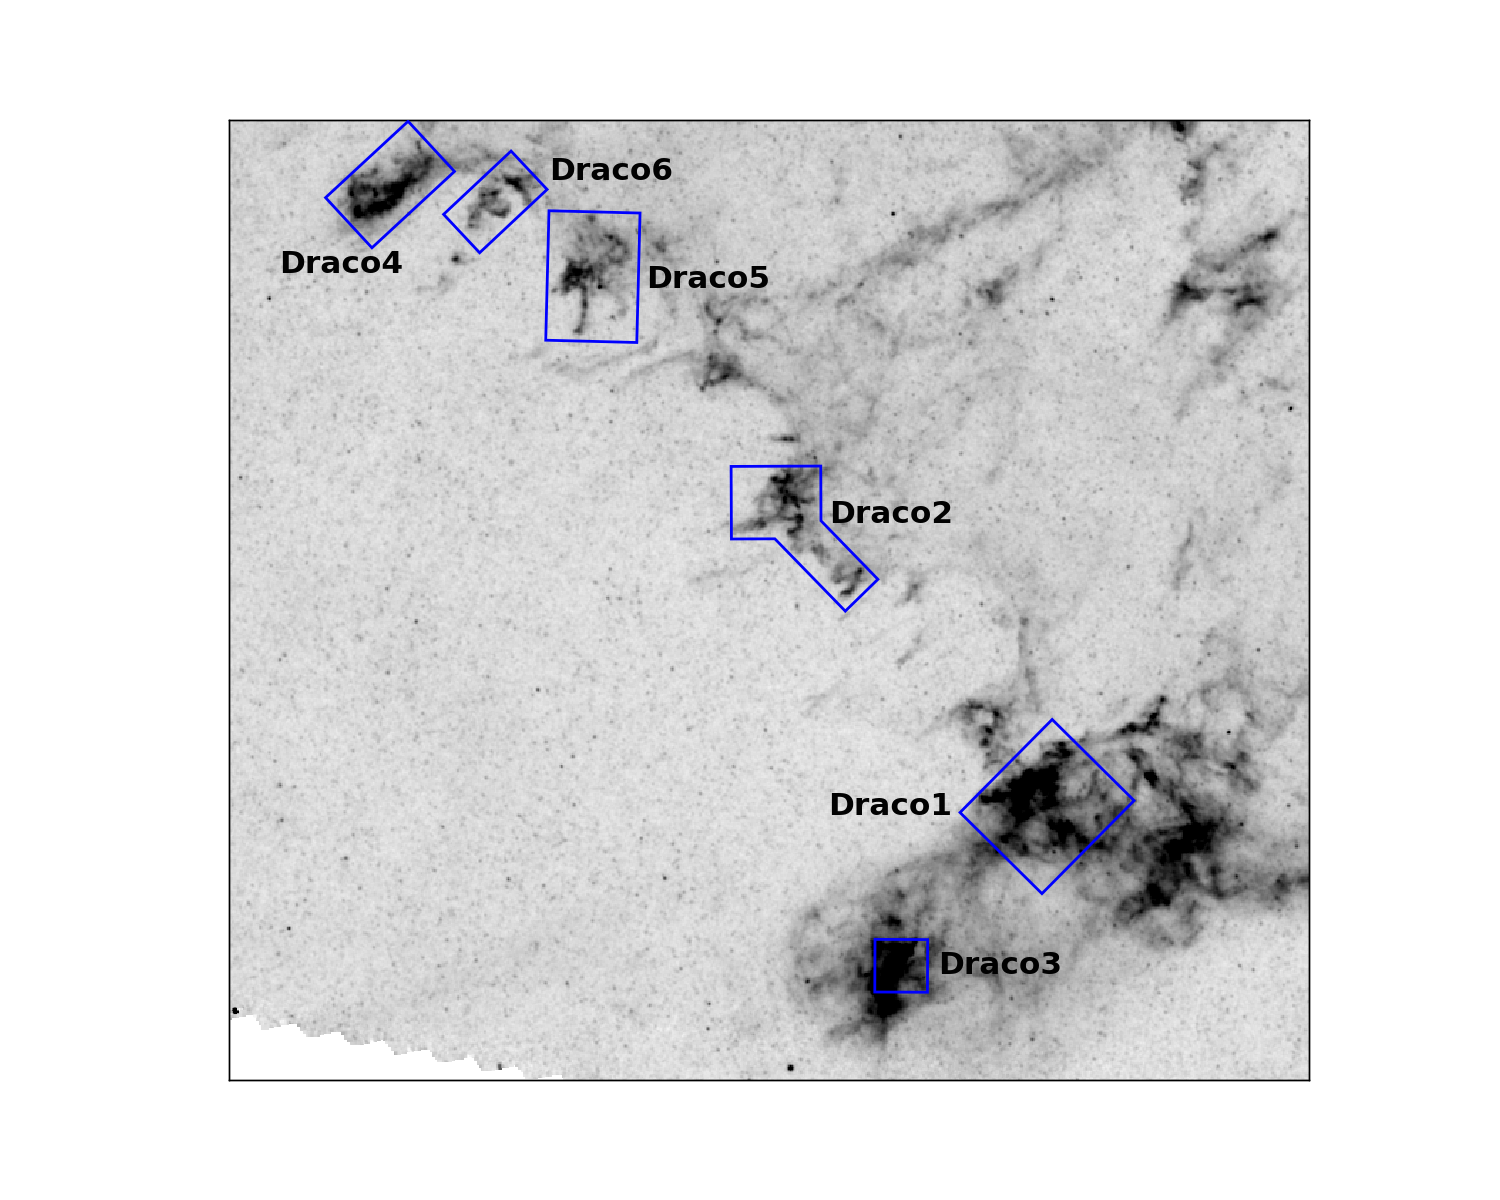
\includegraphics[width=0.7\linewidth,trim=165 85 135 85,clip=true]{Figures/Draco_overview.png}
  \caption{\label{overview} \emph{Herschel}-SPIRE map at $250\: \mu m$ map. The regions observed with the IRAM 30m are represented 
by the boxes.}
\end{figure*}

\begin{table*}[h]
  \centering
  \footnotesize
  \caption{\label{table:rms} Journal of observations at IRAM 30m.}
  \begin{tabular}{lcccccc}
    \hline \hline
    Region &      $\alpha$       &    $\delta$    &        Area         & $t_{obs}$ \tfm{a} & \multicolumn{2}{c}{rms \tfm{b}} \\ \hline 
    Draco1 & $16^h 46^m 39^s.89$ & $+$60:15:52.50 & $16.4'\times 14.4'$ &       18.2h       &    345.4 mK    &    656.3 mK    \\
    Draco2 & $16^h 51^m 16^s.85$ & $+$60:53:43.71 &  157.5 arcmin$^2$   &        8.8h       &    373.1 mK    &    789.8 mK    \\
    Draco3 & $16^h 49^m 06^s.14$ & $+$59:55:59.34 &  $6.6'\times 6.6'$  &        1.1h       &    529.7 mK    &    982.4 mK    \\
    Draco4 & $16^h 58^m 06^s.09$ & $+$61:32:12.85 & $14.0'\times 8.5'$  &        3.7h       &    616.9 mK    &    891.2 mK    \\
    Draco5 & $16^h 54^m 30^s.95$ & $+$61:21:31.45 & $16.2'\times 11.4'$ &        5.0h       &    542.2 mK    &    901.7 mK    \\
    Draco6 & $16^h 56^m 15^s.11$ & $+$61:30:30.70 & $11.6'\times 6.6'$  &        2.3h       &    605.7 mK    &    1.234 K     \\ \hline
%    Draco7 & $16^h 52^m 19^s.99$ & $+$61:10:25.68 &  $8.0'\times 8.0'$  &        0.9h       &    1.536 K     &    3.421 K     \\ \hline
%    Draco9 & $16^h 50^m 28^s.09$ & $+$60:47:11.40 &   54.1 arcmin$^2$   &        1.8h       &    678.8 mK    &    1.093 K     \\ \hline
  \end{tabular}
  \tablefoot{
    \tablefoottext{a}{The effective observing time on-source.}
    \tablefoottext{b}{The rms are given in main beam temperature for a spectral resolution of $\sim 0.13\: km.s^{-1}$. The two values correspond to the peak of the Gaussian that fits the distribution over the pixels in CO(1-0) and CO(2-1).}
  }
\end{table*}

\section{Observations}
\label{sec:Obs}

\subsection{CO emission with IRAM 30m}
Millimetre observations of the CO emission were made with the IRAM 30m telescope on August 2016 and August 2017. 
We observed both the CO(1-0) and CO(2-1) lines simultaneously. We mapped seven regions along the shock front of the Draco nebula 
(see figure \ref{overview}), with a resolution of $22.5''$ for CO(1-0) and $12.3''$ for CO(2-1). The EMIR receiver was used 
simultaneously with the FTS and WILMA backends. In this article, we only present the data acquired with the FTS backend 
(bandwidths of 1.8 GHz; resolution of 50 kHz).
Observations were obtained in on-the-fly mode, with a scanning speed of $\sim 7''/sec$ and a sampling of one scan taken every 0.5s. 
A calibration was done every 10-15 minutes. We scanned the region in two orthogonal directions, with a shift of $\sim 10''$ 
between two scanning lines. Pointing was checked every few hours by observing standard continuum sources and was generally 
determined to be accurate to within a few arc-seconds.
Data reduction was done using the IRAM package CLASS. For each spectra, a linear baseline was subtracted at velocities outside 
the range of the emission line ($-40$ to $-10\: km.s^{-1}$). The last step consists in the creation of the data-cube by 
gridding the spectra and applying a convolution with a Gaussian kernel. The resulting data cubes have median noise levels of 
$350-620\: mK$ for CO(1-0) and $0.6-1.2\: K$ for CO(2-1) at a resolution of $\sim 0.13\: km.s^{-1}$.

%% \begin{figure*}[h]
%%  \centering
%%  \includegraphics[height=6cm,trim=10 35 75 85,clip=true]{/home/qsalome/Draco/CO-data/Pictures/Draco_intensity.png}
%%  \caption{\label{Draco_large} Large scale map of the integrated intensity in $K.km.s^{-1}$ of the CO(1-0) emission. The black contours are the dust emission observed at $250\: mu m$ with \emph{Herschel}-SPIRE.}
%% \end{figure*}
%_______________________________________________________________________________________________________________________________________
%_______________________________________________________________________________________________________________________________________
\subsection{H\rmnum{1} emission with GBT and DRAO}
Draco was observed at 21 cm with the Green Bank Telescope (GBT) and the interferometer of the Dominion Radio Astrophysical 
Observatory (DRAO) as part of the GHIGLS and DHIGLS surveys \citep{Martin_2015,Blagrave_2017}.
A 5\degree$\times $5\degree region was observed with the GBT at a resolution of $9'$. The data-cube we got from the archive 
of GHIGLS data\footnote{\url{www.cita.utoronto.ca/GHIGLS}} covers the velocity range $-450\leq v_{LSR}\leq 400\: km.s^{-1}$. 
The average noise level of the map is 60 mK at $0.8\: km.s^{-1}$ resolution.
The GHIGLS data were then used by \cite{Blagrave_2017} for the low spacing of the DRAO data. A region of $12.5\: deg^2$ 
was covered with the DRAO at a resolution of $61''\times 53.7''$. The data-cube from the archive of 
DHIGLS data\footnote{\url{www.cita.utoronto.ca/DHIGLS}} covers the velocity range $-165\leq v_{LSR}\leq 45\: km.s^{-1}$. 
The typical rms is 105 mK at $0.8\: km.s^{-1}$ resolution.
We refer to \cite{Martin_2015} and \cite{Blagrave_2017} for more details.

\section{Results}
\label{sec:Res}
\subsection{H\rmnum{1} emission}
\label{sec:HI-data}
\begin{figure}
   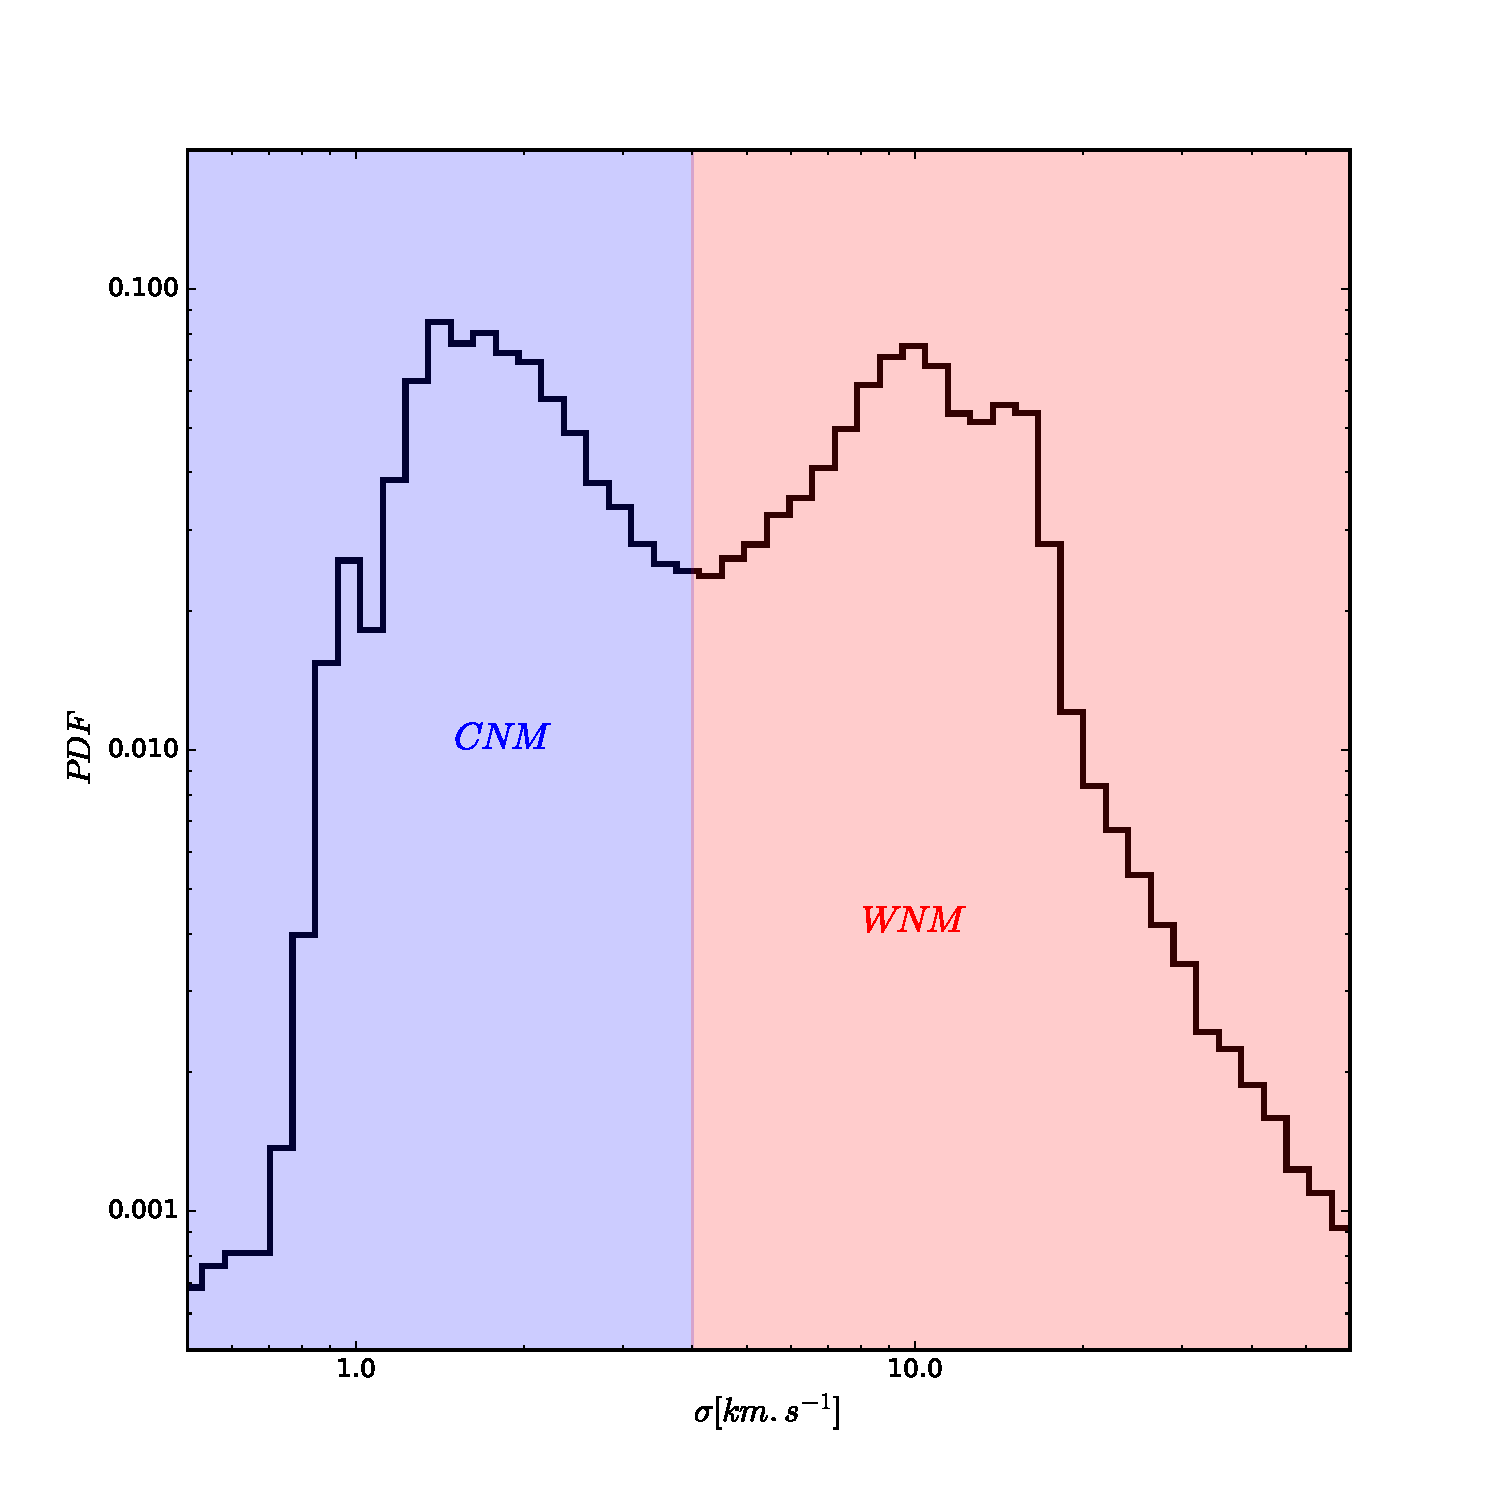
\includegraphics[width=\linewidth]{Figures/PDF_sigma_over_A.pdf}
   \caption{PDF of the dispersion $\sigma_{obs}$ of the Gaussian sample weighted by the amplitude times the dispersion $A\sigma$ 
     after the coherent decomposition of \textit{DRACO}.}
   \label{fig::PDF_sigma_over_A}
\end{figure}

\begin{figure}
   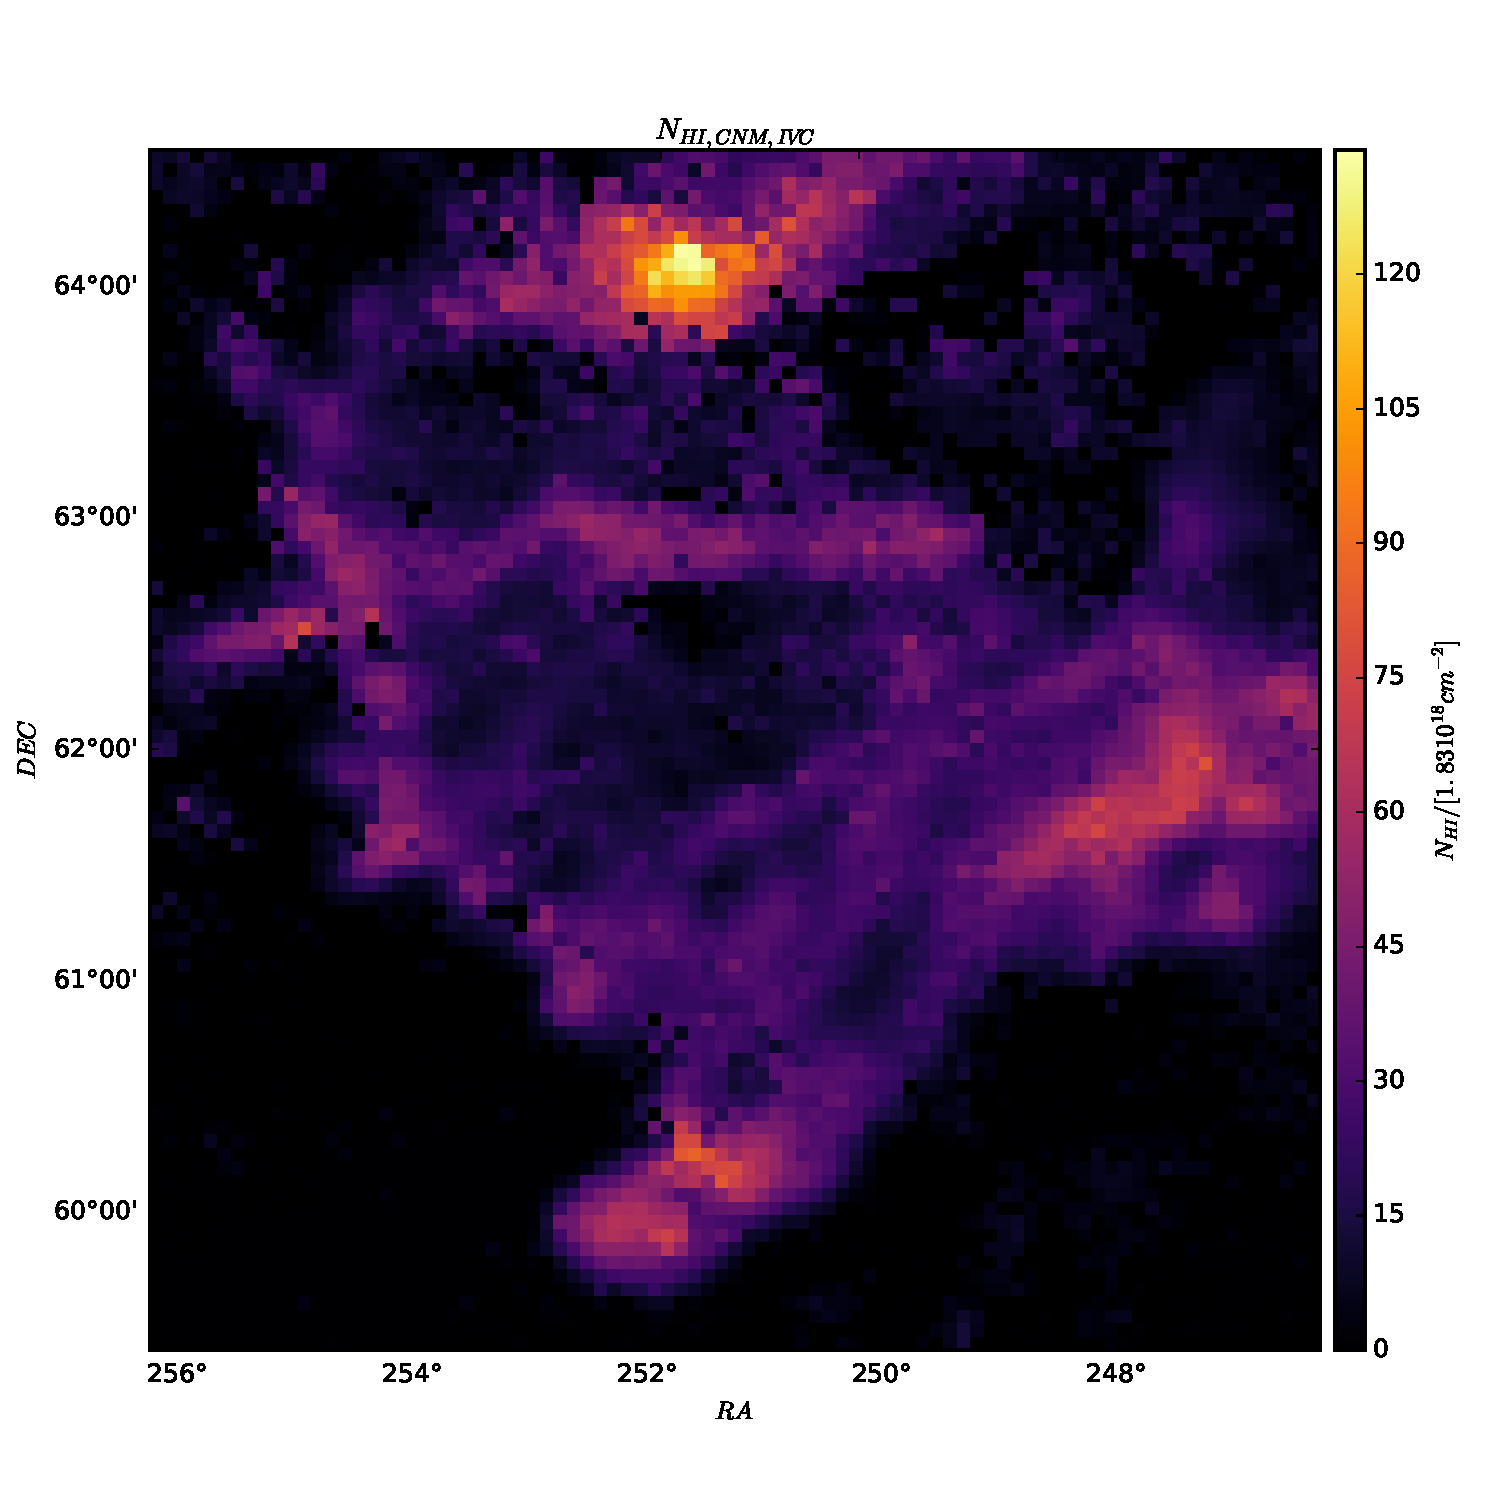
\includegraphics[width=\linewidth]{Figures/NHI_obs_CNM_IVC.pdf}
   \caption{Estimated column density $N_{HI, CNM, \textit{DRACO}, IVC}$ of the Cold Neutral Medium of the IVC of \textit{DRACO}.}
   \label{fig::NHI_obs_CNM_IVC}
\end{figure}
\begin{figure}
   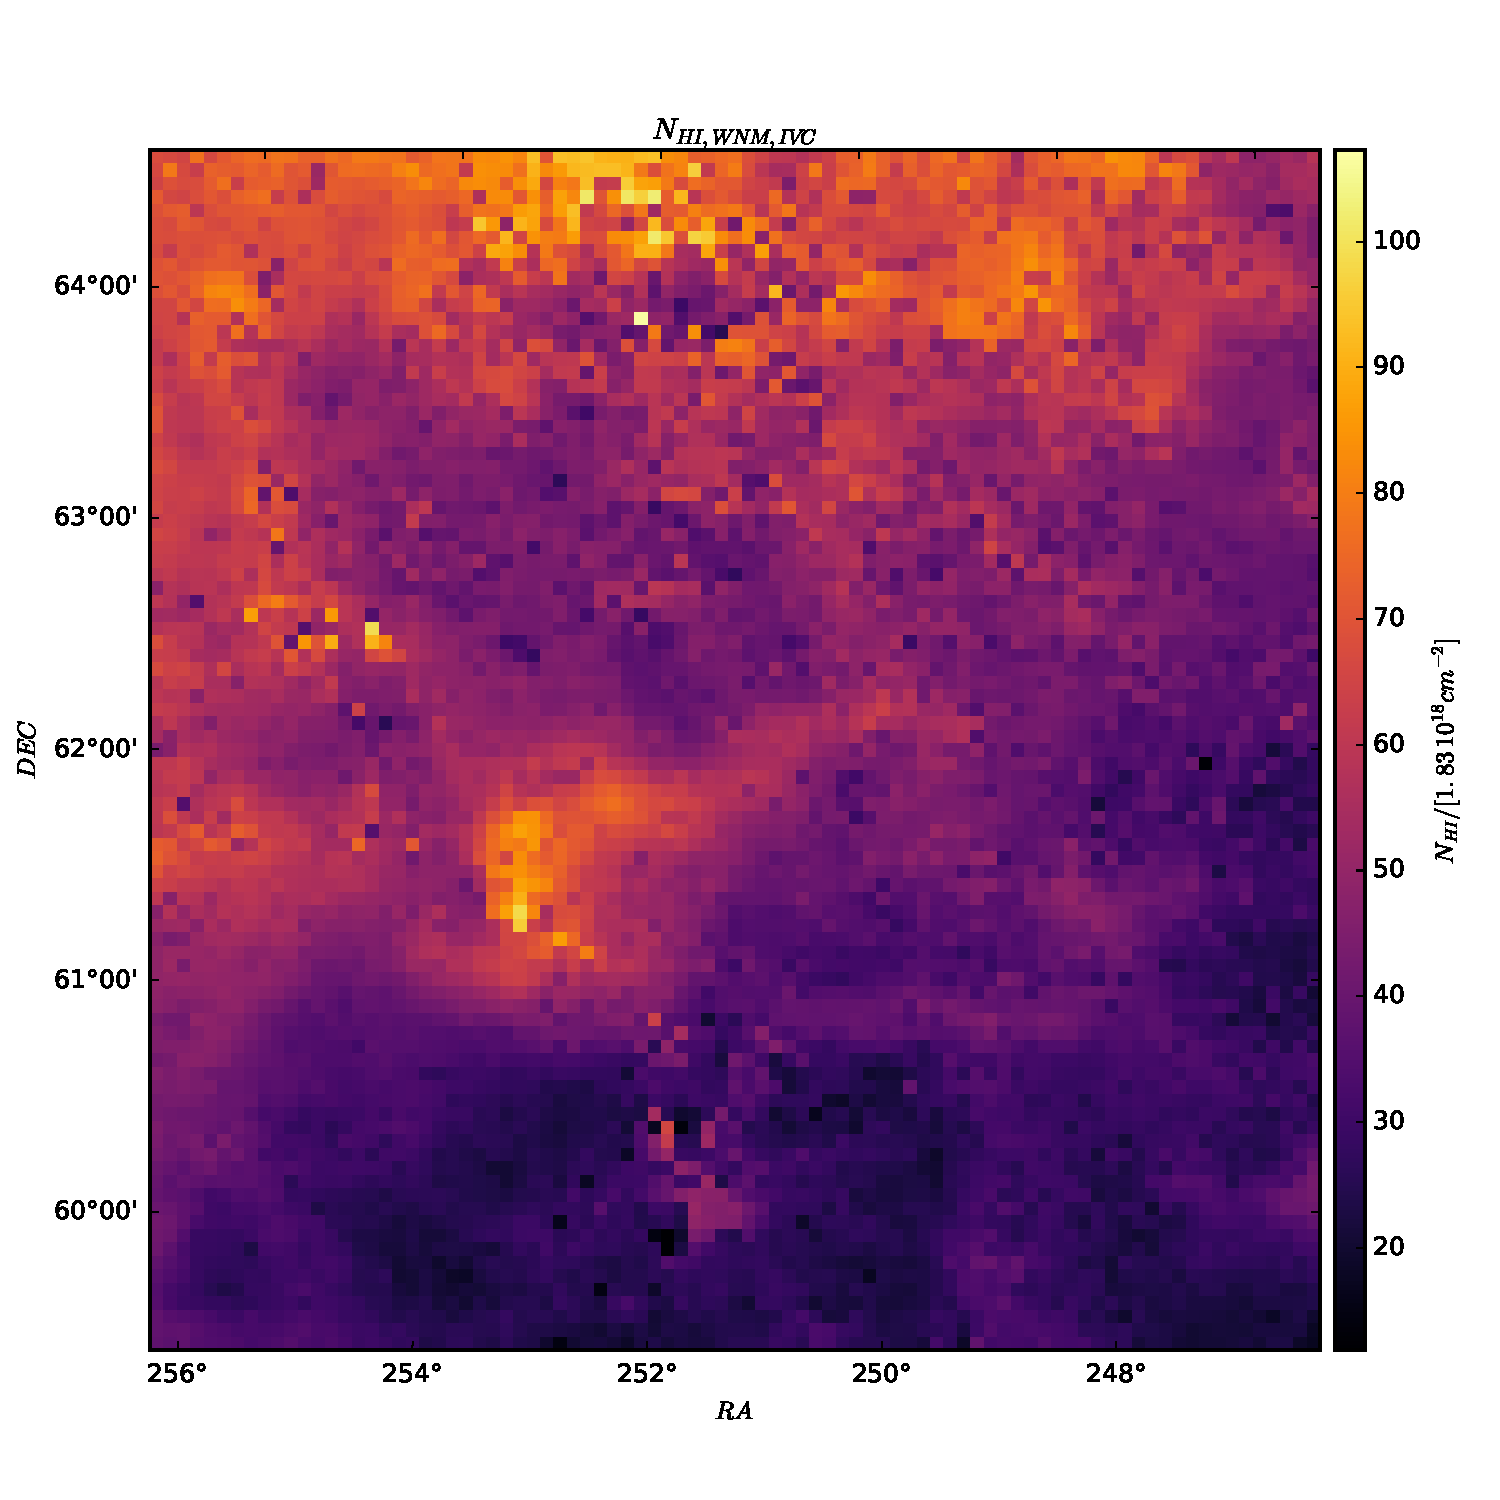
\includegraphics[width=\linewidth]{Figures/NHI_obs_WNM_IVC.pdf}
   \caption{Estimated column density $N_{HI, WNM, \textit{DRACO}, IVC}$ of the Warm Neutral Medium of the IVC of \textit{DRACO}.}
   \label{fig::NHI_obs_WNM_IVC}
\end{figure}
\begin{figure}
   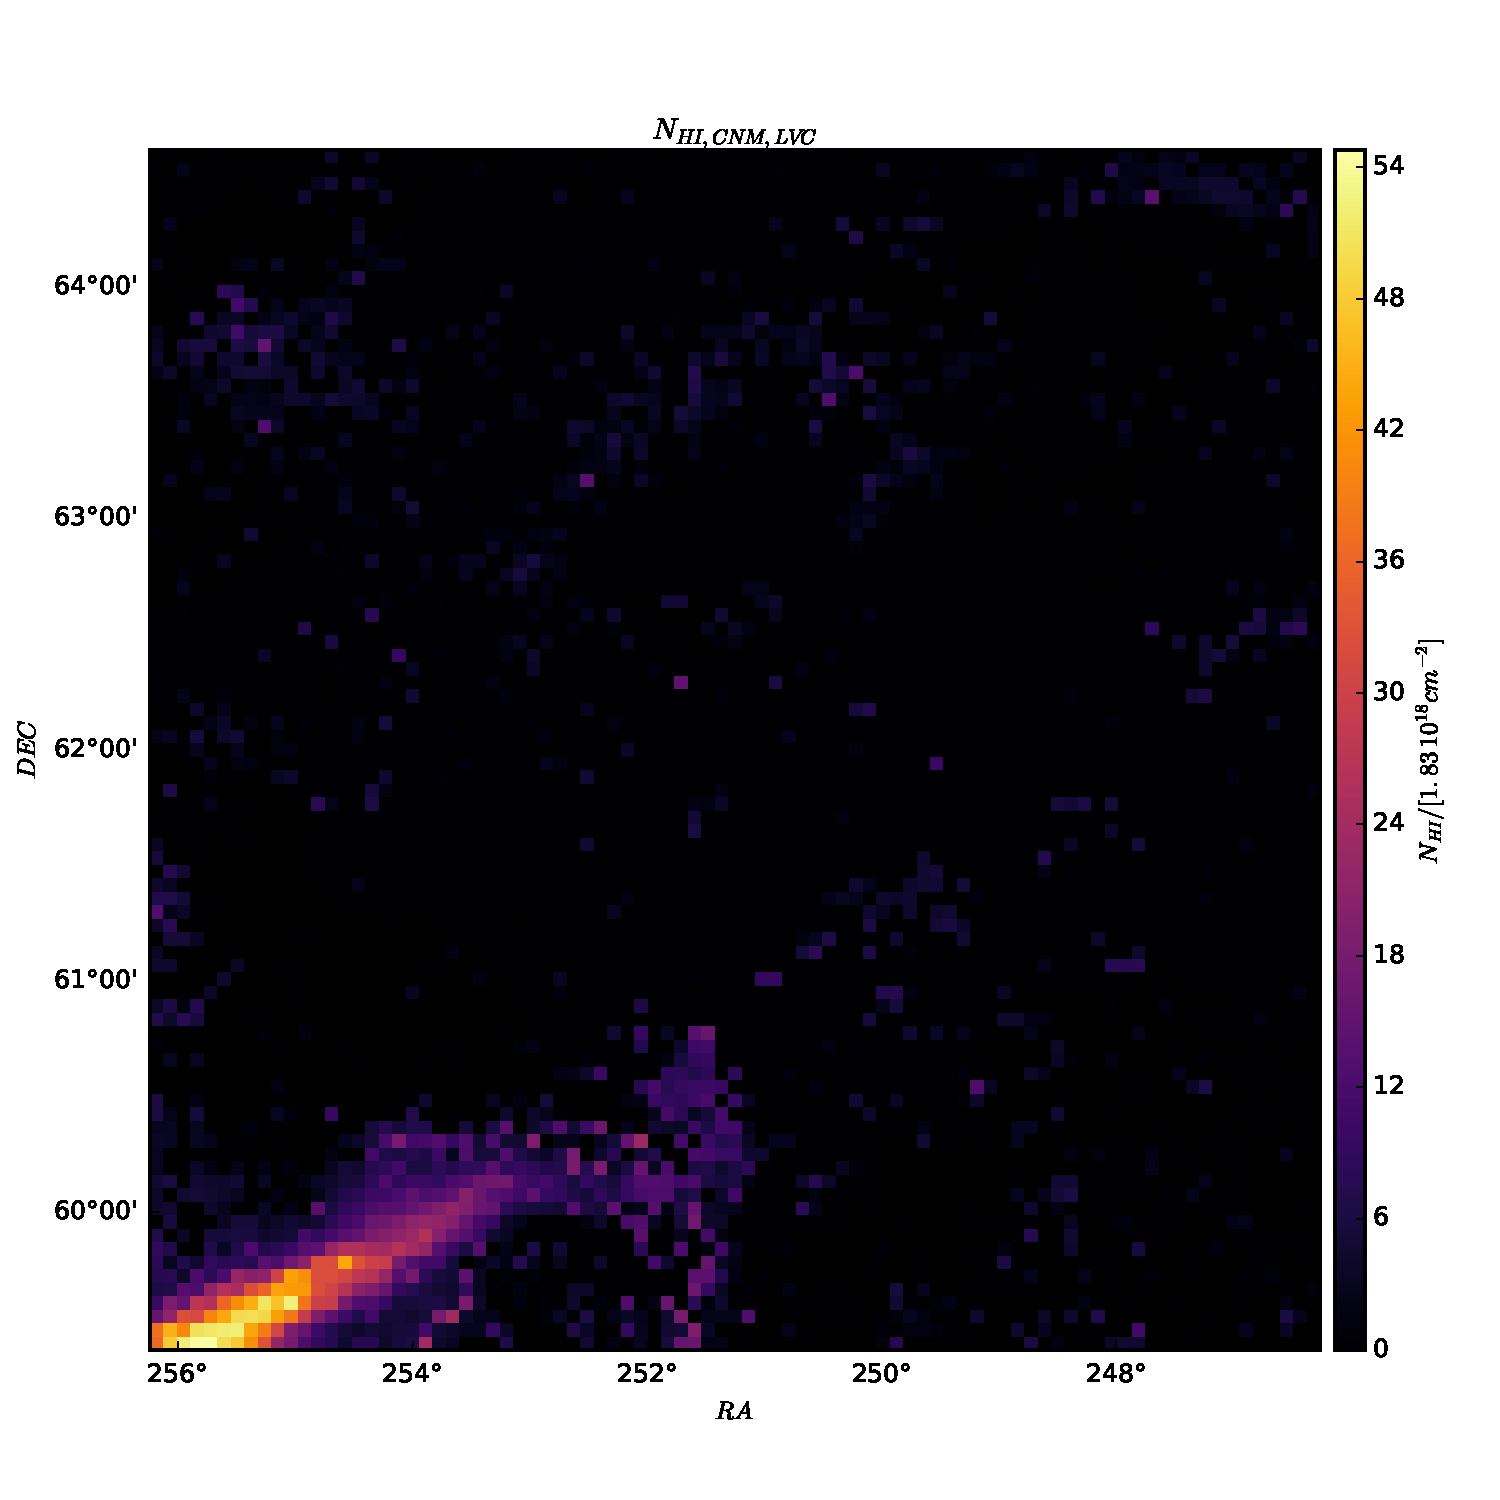
\includegraphics[width=\linewidth]{Figures/NHI_obs_CNM_LVC.pdf}
   \caption{Estimated column density $N_{HI, CNM, \textit{DRACO}, LVC}$ of the Cold Neutral Medium of the LVC of \textit{DRACO}.}
   \label{fig::NHI_obs_CNM_LVC}
\end{figure}
\begin{figure}
   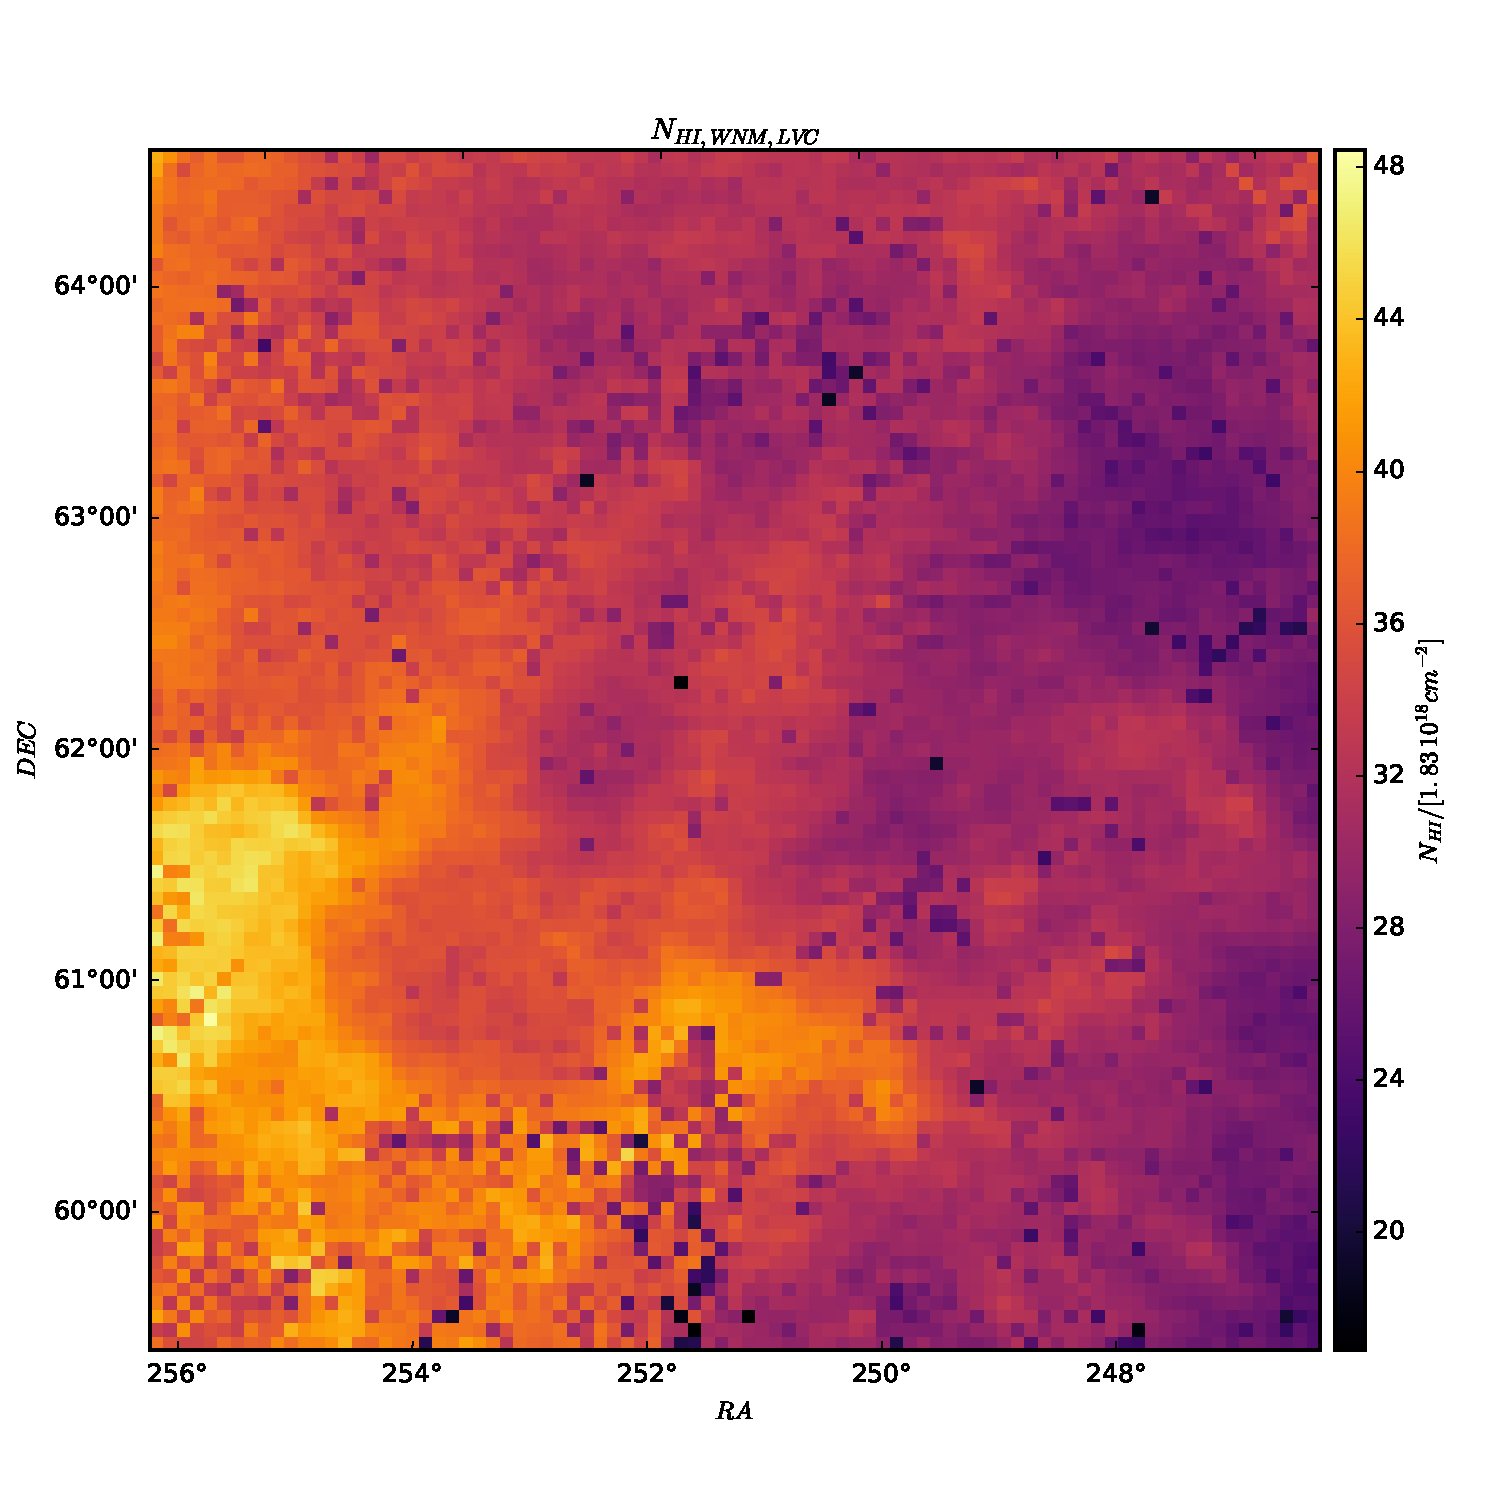
\includegraphics[width=\linewidth]{Figures/NHI_obs_WNM_LVC.pdf}
   \caption{Estimated column density $N_{HI, WNM, \textit{DRACO}, LVC}$ of the Warm Neutral Medium of the LVC of \textit{DRACO}.}
   \label{fig::NHI_obs_CNM_LVC}
\end{figure}

\begin{figure*}
   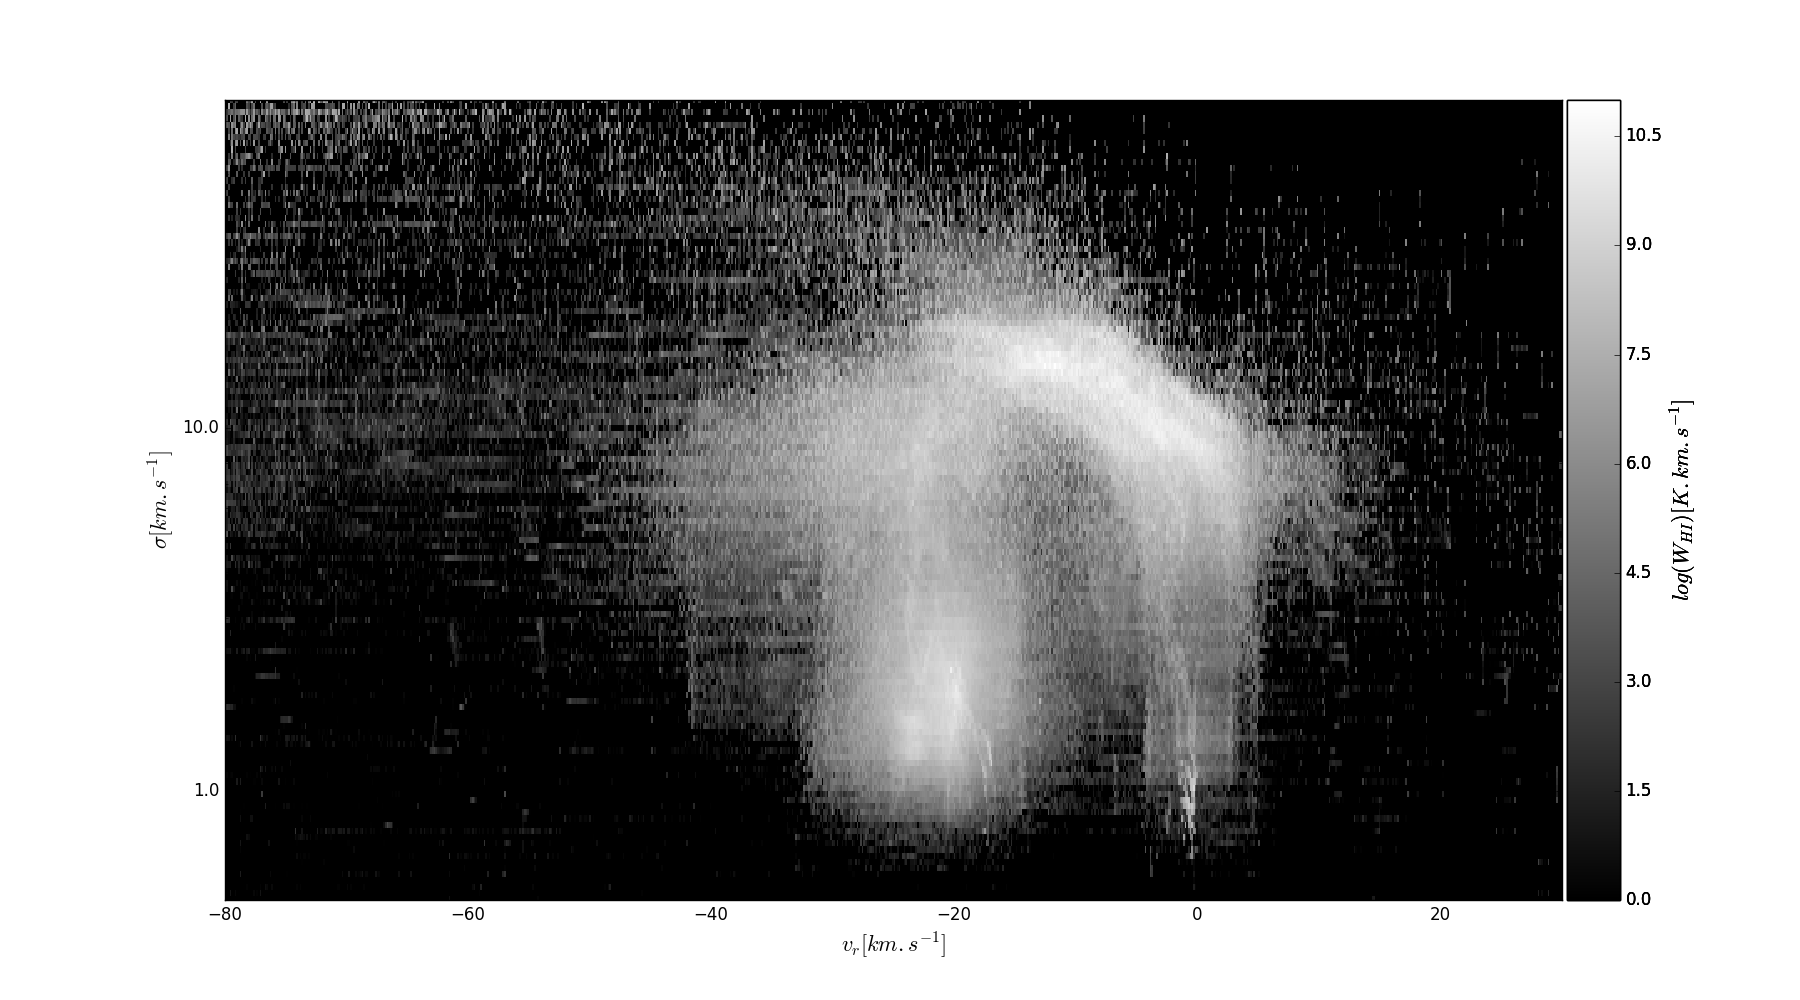
\includegraphics[width=\linewidth]{Figures/heatmap_png.png}
   \caption{Histogram of the dispersion $\sigma$ and the mean position $v_{r}$ of the Gaussian sample of \textit{DR}.}
   \label{fig::heatmap}
\end{figure*}

\begin{figure*}[h!]
   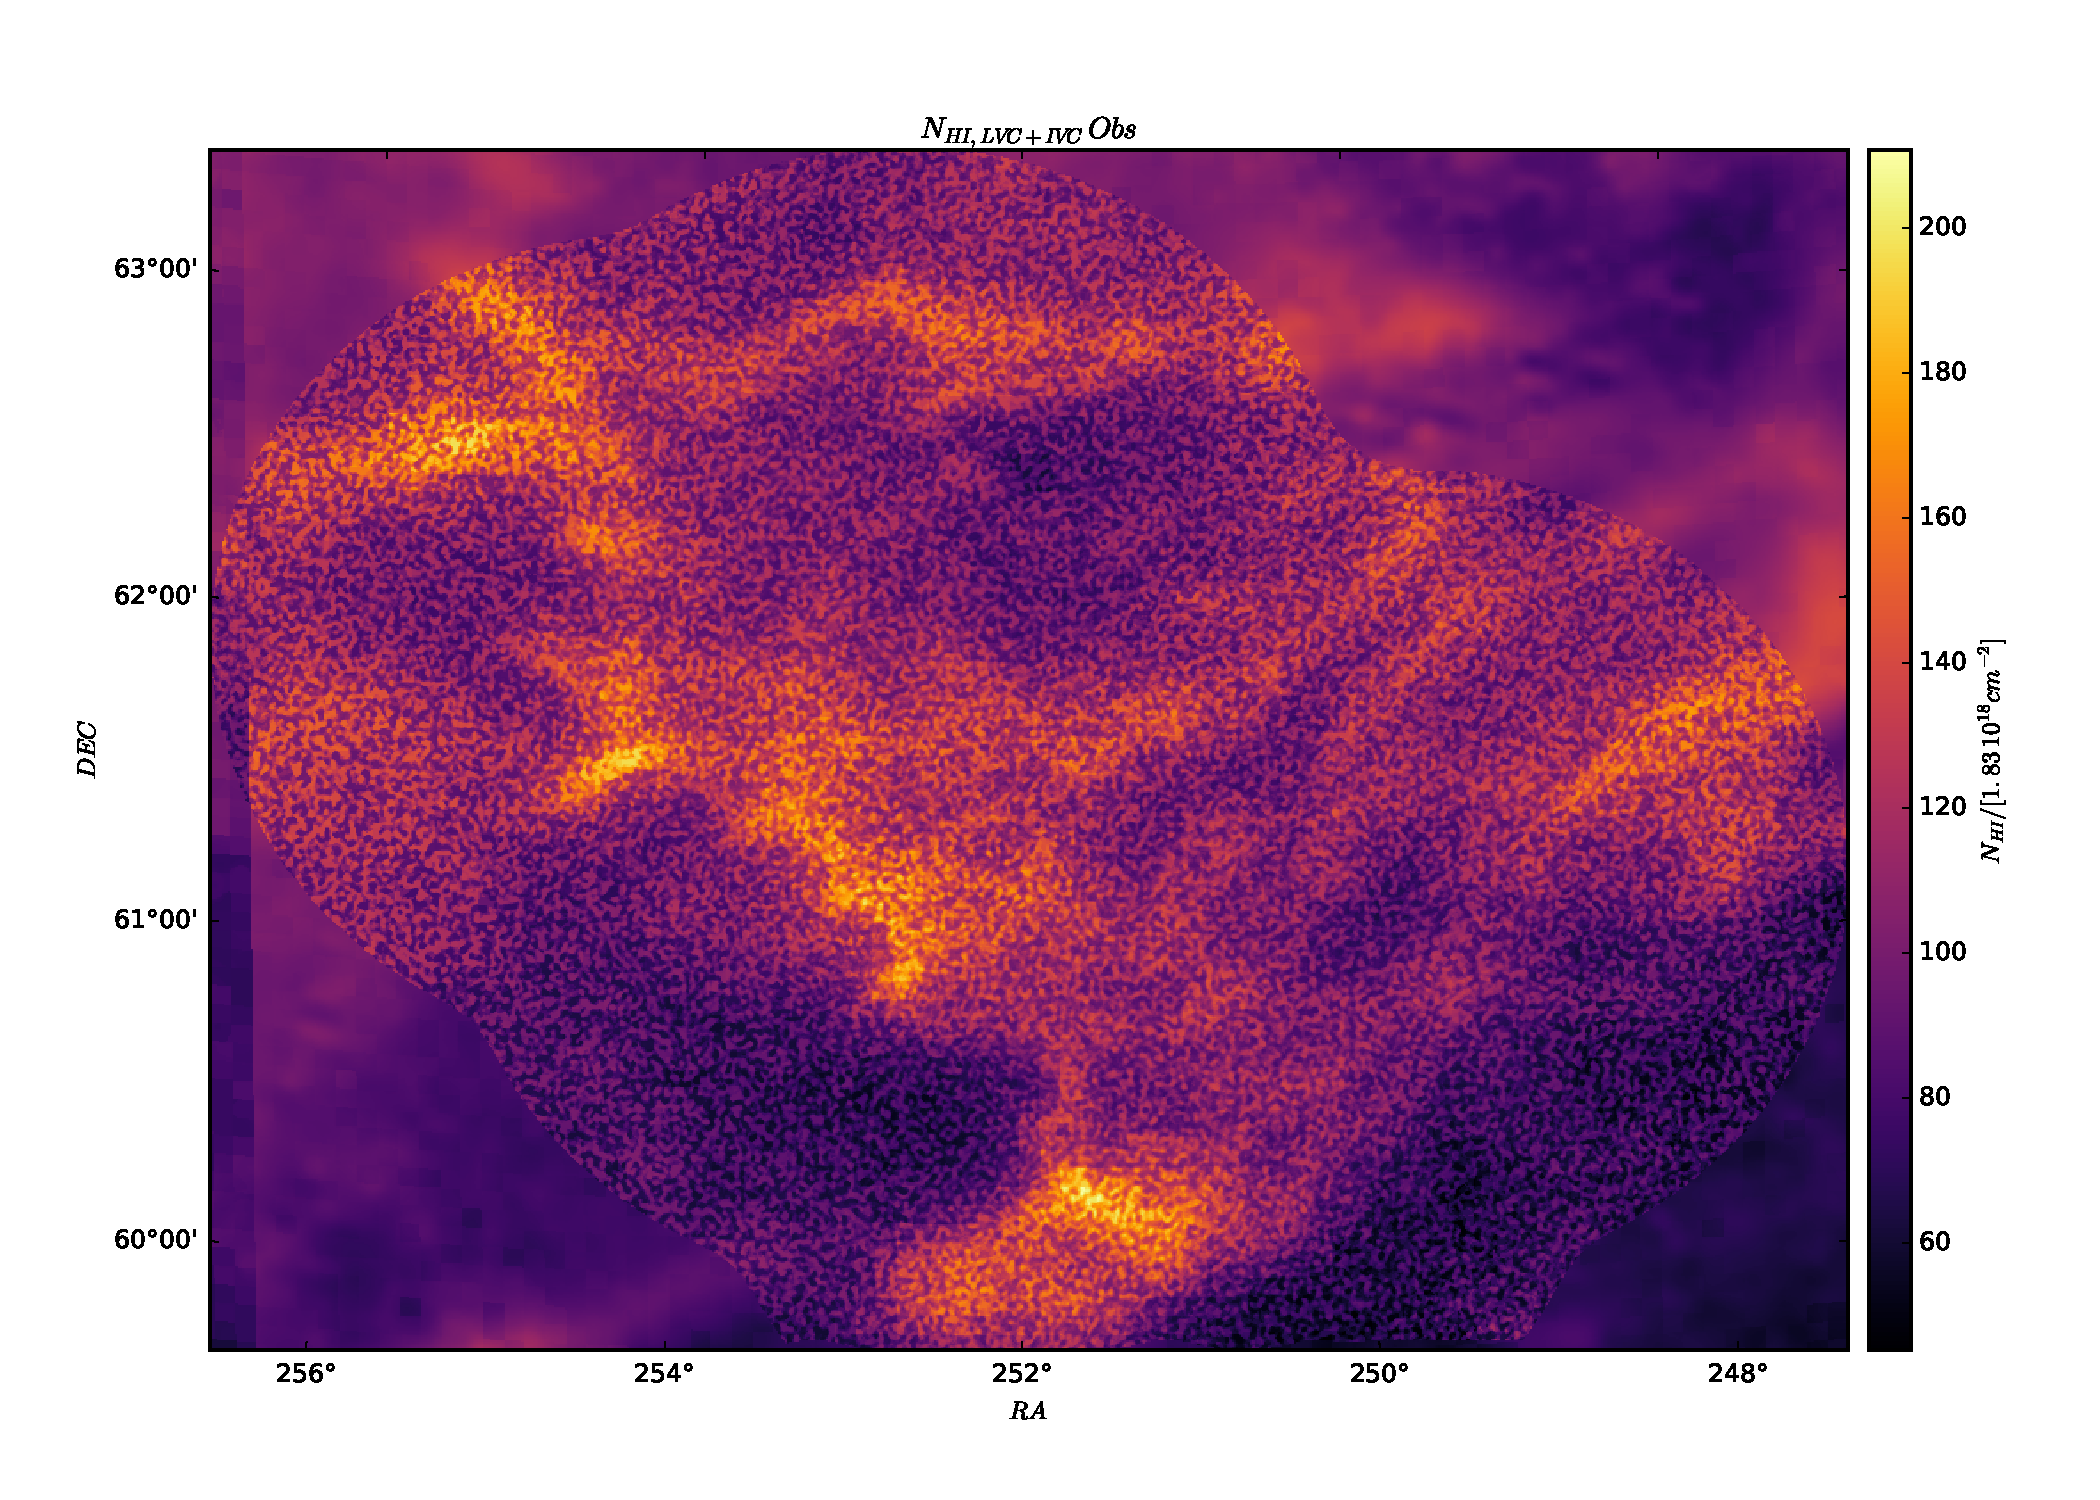
\includegraphics[width=\linewidth]{Figures/NHI_obs_DRAO.pdf}
   \caption{Estimated total column density $N_{HI, DR, LVC+IVC}$ of the Neutral Medium of the LVC+IVC of \textit{DR}.}
   \label{fig::NHI_obs_DRAO}
\end{figure*}

Understand the structure and the dynamic of the neutral material in the Draco Nebula is a key point to establish a scenario about
its history. \cite{field1969cosmic} has postulated a ``two phase'' model to describe the neutral hydrogen in the ISM : 
A cold (T$\sim$50K, n$\sim$50$cm^{-3}$) dense phase, the cold neutral medium (CNM) and a diffuse warm (T$\sim$8000K, 
n$\sim$0.1$cm^{-3}$) phase, the warm neutral medium (WNM). This model, from the large galactic scale to the 
small cloud scale, is omnipresent in galaxies (\color{red} maybe refs \color{black}).
Using the H\rmnum{1} observations, we aim to probe these phases along the line-of-sight of the field. In order to make a clear 
distinction between GBT field and DRAO field we will use the name given by \cite{Martin_2015} and \cite{Blagrave_2017} namely 
respectively \textit{DRACO} and \textit{DR}. For each line of sight, we estimate $N_{HI}$ from 21 cm measurements which is 
the integral of the density fluctuations (see Marchal et al. in prep. for details about the theoretical considerations). \\
\begin{align}
  \frac{N_{HI}}{cm^{-2}} &= 1.82243 \times 10^{18} \times \int_{-\infty}^{+\infty} \left( \frac{T_B(u)}{K} 
  \right) \, d\left( \frac{u}{km.s^{-1}}\right) 
  \label{eq::NHI}
\end{align}

\noindent
where $T_B(u)$ is the brightness temperature at velocity $u$.

\subsubsection{Data processing}
We applied a coherent multi-Gaussian decomposition (see Marchal et al. in prep. for details) in order to separate them. 
The high noise level of \textit{DR} enables to only recover the signal from the CNM. Moreover, the Gaussian decomposition 
method fits noise peaks that makes the result unusable. We nevertheless succeed to infer the two phase component of the Draco Nebula 
using \textit{DRACO} as a first step. Indeed, when applied to the GHIGLS data, the Gaussian decomposition method well 
recovers the two phases. In particular, the distribution of the width $\sigma$ (see figure \ref{fig::PDF_sigma_over_A}), indicates 
that both cold and warm phases are recovered. With the set of Gaussian obtained from \textit{DRACO} we re-project them on the DR grid 
in order to refit the solution while constraining the parameter space of each Gaussian with +/- ten percent of the initial solution. 
Therefore, we adjusted the coherent decomposition while avoiding to fit noise in the data. Furthermore, as shown in figure 
\ref{fig::PDF_sigma_over_A} we choosed $\sigma_{lim, \, \textit{DRACO}} = 4 \, km.s^{-1}$ to be the quantitative separation between 
cold and warm phases. We note that, by construction, $\sigma_{lim, \, \textit{DRACO}} = \sigma_{lim, \, \textit{DR}}$. Then, for every 
line-of-sight, we infer each new hyper-spectral cube summing all Gaussian lower than $\sigma_{lim, \, \textit{DRACO}}$ for the CNM 
and greater than $\sigma_{lim, \, \textit{DRACO}}$ for the WNM. Finally, we can integrate each of them, using equation \ref{eq::NHI} 
to obtain the integrated column density maps of each phases, $N_{HI, \, CNM, \, \textit{DRACO}, \, IVC}$, 
$N_{HI, \, WNM, \, \textit{DRACO}, \, IVC}$, $N_{HI, \, CNM, \, \textit{DRACO}, \, LVC}$, 
$N_{HI, \, WNM, \, \textit{DRACO}, \, LVC}$ which are presented figure \ref{fig::NHI_obs_CNM_IVC}, \ref{fig::NHI_obs_WNM_IVC}, 
\ref{fig::NHI_obs_CNM_LVC} and \ref{fig::NHI_obs_CNM_LVC}. Note that we used the values of \cite{Planck_XXIV_2011} ($-8.8 < v_{LVC} \, [km.s^{-1}] < 24.1$; $-73.1 <v_{IVC} \, [km.s^{-1}] < -8.8$). 
to separate the local velocity component (LVC) to the intermediate velocity component (IVC). The total integrated column density map of \textit{DR} for the LVC+IVC 
is presented figure \ref{fig::NHI_obs_DRAO}. Furthermore, in order to understand the dynamics of the gas, an histogram of the 
dispersion $\sigma$ and the mean position $v_{r}$ of the Gaussian sample of \textit{DR} is shown figure \ref{fig::heatmap}.

\subsubsection{Data analysis}

%% \begin{figure*}[h]
%%   \centering
%%   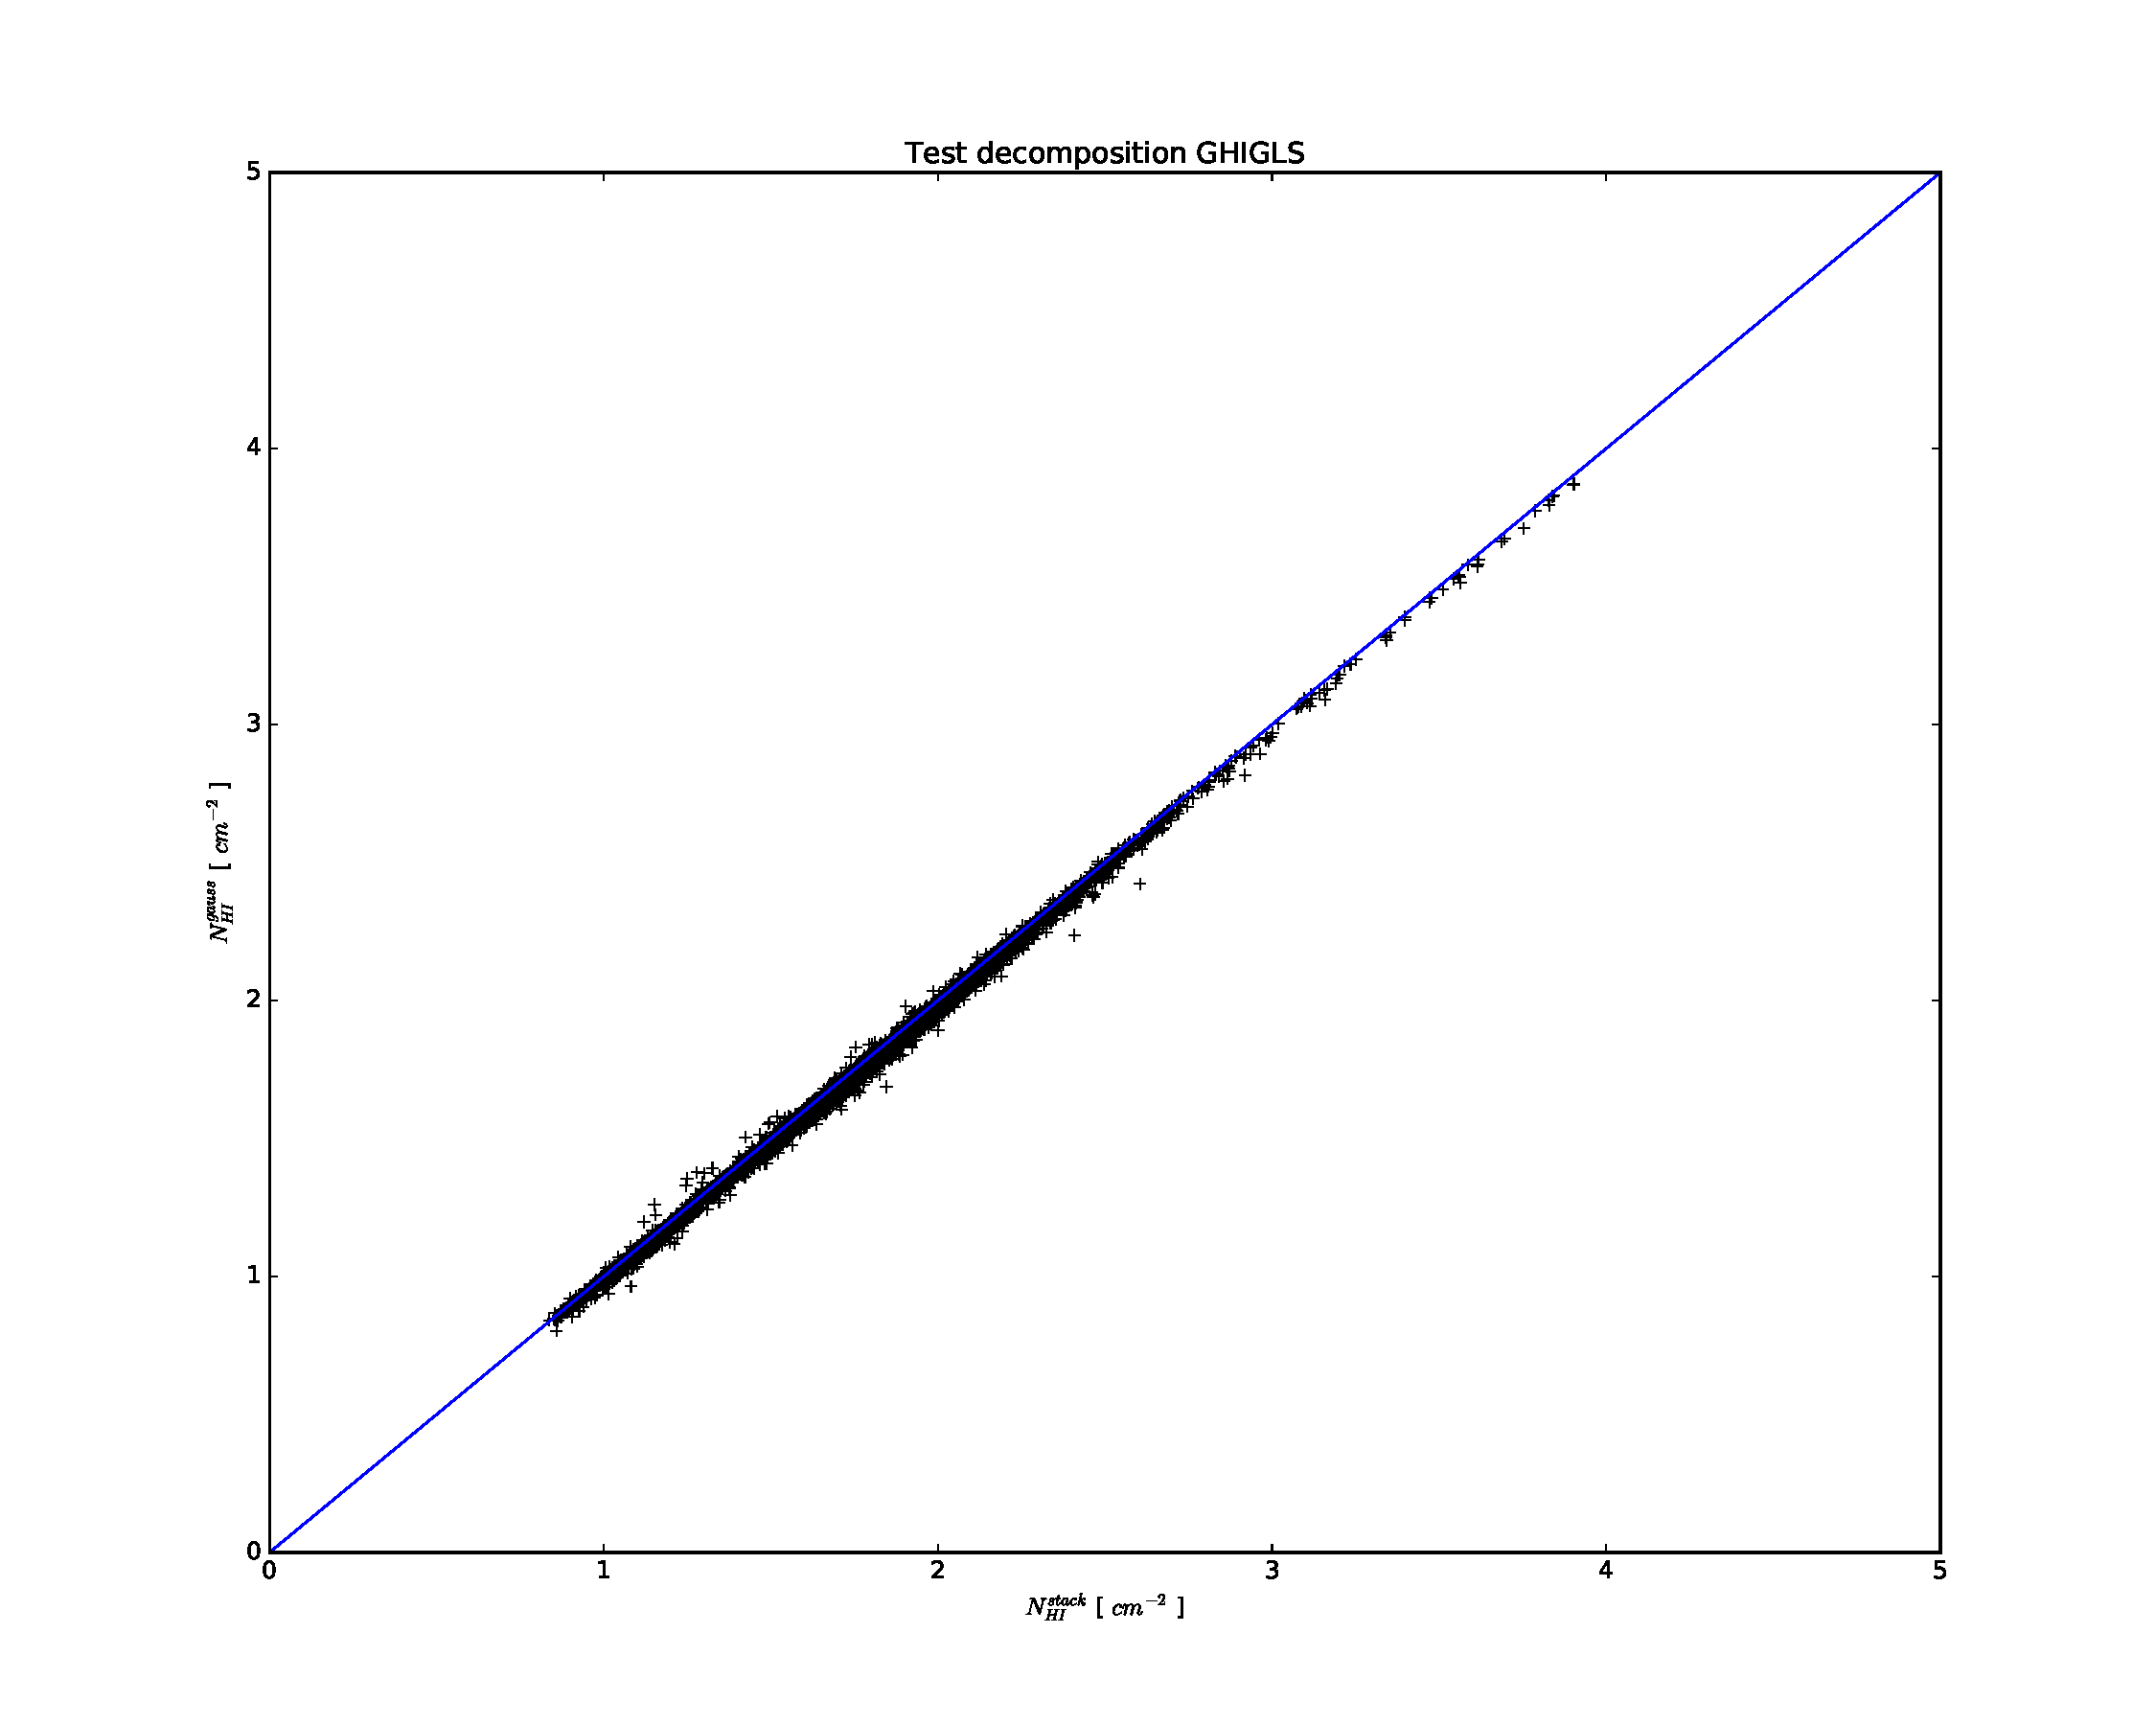
\includegraphics[page=1,height=6.5cm,trim=10 55 60 90,clip=true]{Figures/Test_decomposition.pdf}
%%   \hspace{3mm}
%%   \includegraphics[page=3,height=6.5cm,trim=10 55 60 90,clip=true]{Figures/Test_decomposition.pdf}
%%   \caption{Comparison of the flux reconstructed by the coherent gaussian decomposition for GHIGLS and DHIGLS. The blue line is the 
%%     1:1 slope.}
%% \end{figure*}

%% \subsection{Dynamics}
%% The multi-Gaussian decomposition method from Marchal et al. (in prep.) provides a list of Gaussians. Each Gaussian is characterised 
%% by its position $\mathnormal{x}$,$\mathnormal{y}$, its amplitude $\mathnormal{A}$, its position $\mathnormal{\mu}$, and its width 
%% $\mathnormal{\sigma}$. In order to compute the velocity map, we first reconstruct the signal in each pixel:

%% \begin{equation}
%%   \mathnormal{T_b(v)=\sum_{i=1}^{N_{comp}} A_i \exp\cbra{(v-v_i)^2/2\sigma_i^2}}
%% \end{equation}

%% We then computed the emission-weighted mean velocity $\avg{v}$ and the velocity dispersion $\sigma_v$:
%% \begin{equation}
%%   \mathnormal{\avg{v}=\frac{\sum_v v\, S_{CO}^{tot}(v)\, dv}{\sum_v S_{CO}^{tot}(v)}}
%% \end{equation}
%% \begin{equation}
%%   \mathnormal{\sigma_v=\sqrt{\frac{\sum_v v^2\, S_{CO}^{tot}(v)\, dv}{\sum_v S_{CO}^{tot}(v)}-\avg{v}^2}}
%% \end{equation} 
%% where $\mathnormal{dv}$ is the channel width.

%% \subsubsection{Large scale dynamics (HI)}
%% The resulting velocity map is represented in figure \ref{Draco_HI}. The velocity gradient observed in H\rmnum{1} at the interface 
%% with the Rayleigh-Taylor instability strengthens the scenario of a shock between the cloud at the origin of Draco and the warm neutral 
%% medium (WNM) of the Galactic disc. Surprisingly, the bright structure in the south has velocities larger than the rest of the nebula.
%___________________________________________________________________________________________________________________________________
%___________________________________________________________________________________________________________________________________
\newpage
\subsection{CO emission}
\subsubsection{Morphology}

For such a diffuse high latitude cloud, CO is very bright in the regions observed with the IRAM 30m telescope. The CO(1-0) line peaks between 1 K and 12 K, while the CO(2-1) line peaks between 0.5 and 9 K. In all the regions, CO emission shows small structures embedded within more extended, diffuse molecular gas. Moreover, the peaks of CO emission are spatially correlated to the $250\: \mu m$ dust emission from Herschel (figure \ref{Draco_CO10}), indicating that both components are likely related. Below, we quickly present the CO morphology in the different regions we observed.
\medskip

\noindent \textit{Draco1} - Located in the southern part of the Draco nebula, this region covers one of the bright dusty structures seen with Herschel. It corresponds to the CO-clumps referred as Drop by \cite{Mebold_1985}. Our integrated intensity map shows three bright, extended structures. One of these seems to contains four bright CO clumps that are aligned with the dust emission. Finally, in the southern part of the map, there is two faint, extended structures that are co-spatial with dust emission.
\medskip

\noindent \textit{Draco2} - This region is located about at the center of the shock front. It corresponds to some flat dusty front structure. CO emission reveals four bright and one fainter separated structures co-spatial with dust emission.
\medskip

\noindent \textit{Draco3} - Focused on the northern part of the Wart clump of \cite{Mebold_1985}, the CO observations reveal a very bright, large structure at the centre and two fainter, smaller structures in the north. The three structures are co-spatial with a peak of dust emission.
\medskip

\noindent \textit{Draco4} - We mapped the entire clumps referred as Fang by \cite{Mebold_1985}. This structure lies at the edge of the shock front. CO is mostly emitted by a diffuse structure that follows dust emission. There is also a bright structure where the structure is thinner on the sky.
\medskip

\noindent \textit{Draco5} - Dust emission in this region has a very peculiar shape. Dust emission is bright at the centre, extended in the north and shows a tail-like structure in the south. CO was detected along the entire structure, including in the tail. CO emission is brighter in the centre and presents some clumpy structures bathed in diffuse, extended molecular gas.
\medskip

\noindent \textit{Draco6} - The last region present a few bright structures in both CO and dust emission. In particular there is an elongated bright structure in the north.


\subsubsection{CO-to-H$_2$ conversion factor}
We used the CO-dust coherence to estimate a CO-to-$H_2$ conversion factor $X_{CO}$ in both regions. To do so, we compared the CO intensity $I_{CO}$ with the total column density $N(H)$, derived from the \emph{Herschel} dust emission, and the H\rmnum{1} column density $N(H\rmnum{1})$. \cite{MAMD_2017b} shows that the $250\: \mu m$ intensity is strongly correlated with the optical depth at $353\: GHz$ from \emph{Planck}. The authors concluded that the total column density is given by:

\begin{figure*}[h]
  \centering
  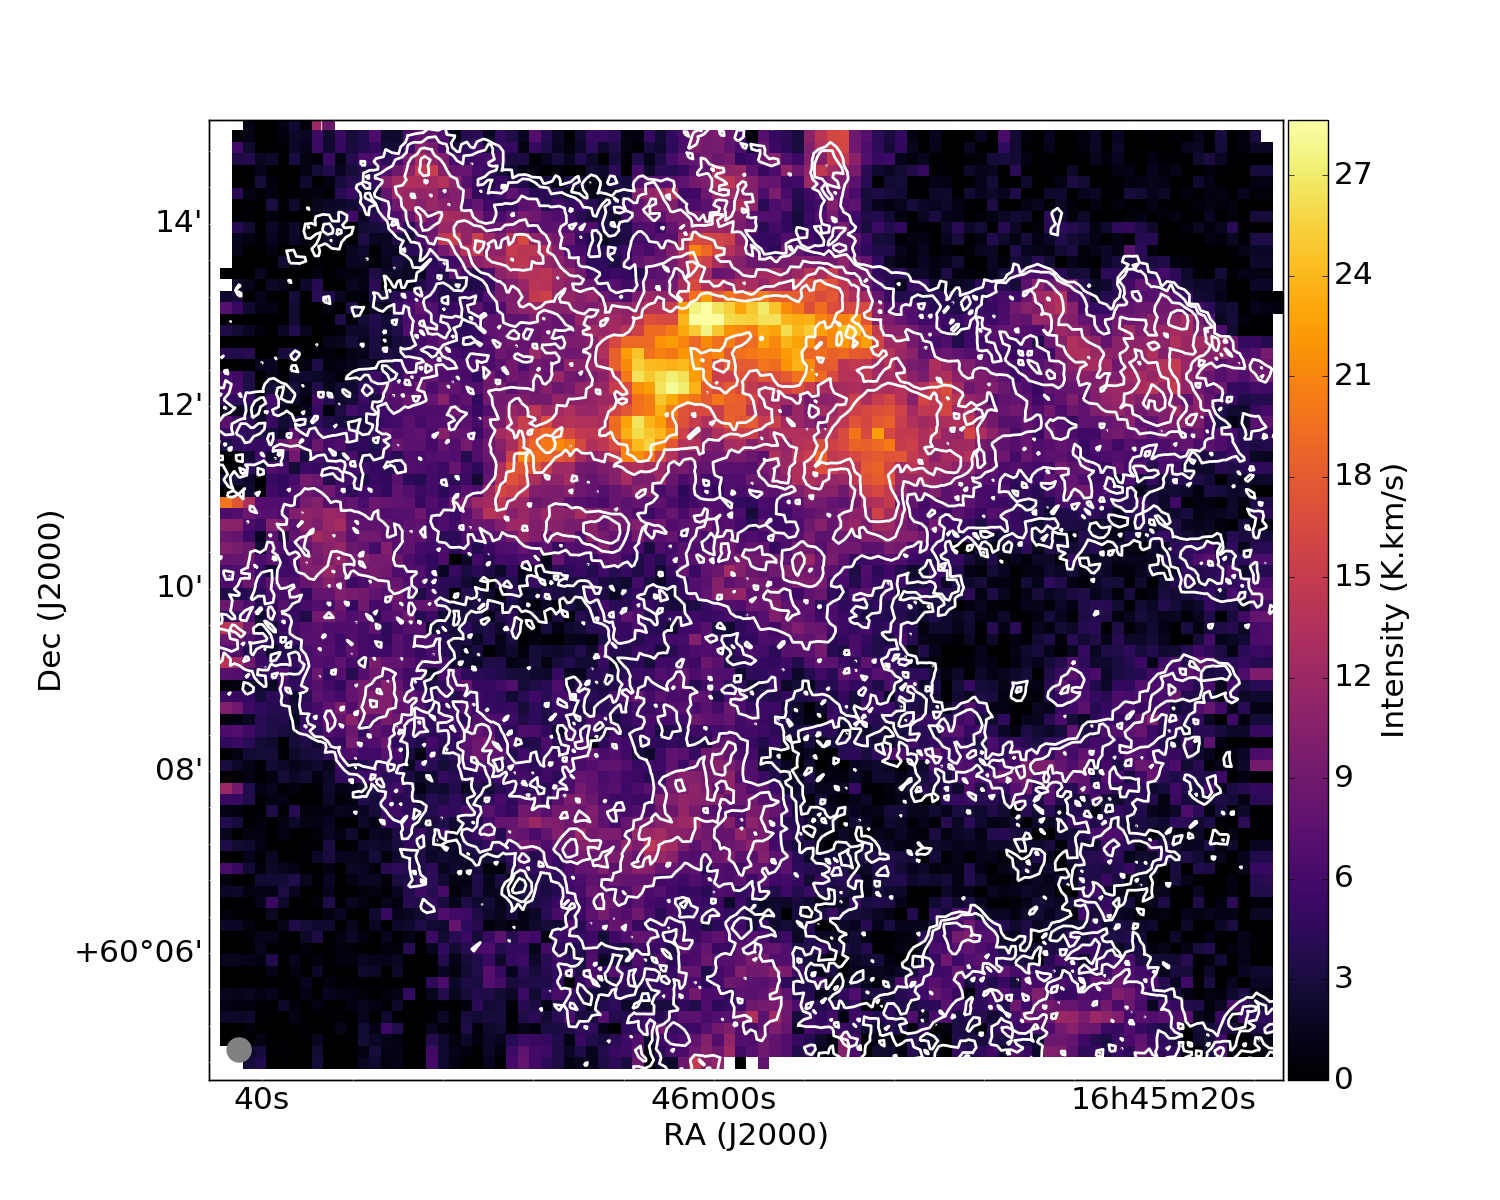
\includegraphics[height=4.5cm,trim=50 40 50 40,clip=true]{Figures/Draco1_stack.png}
  \hspace{3mm}
  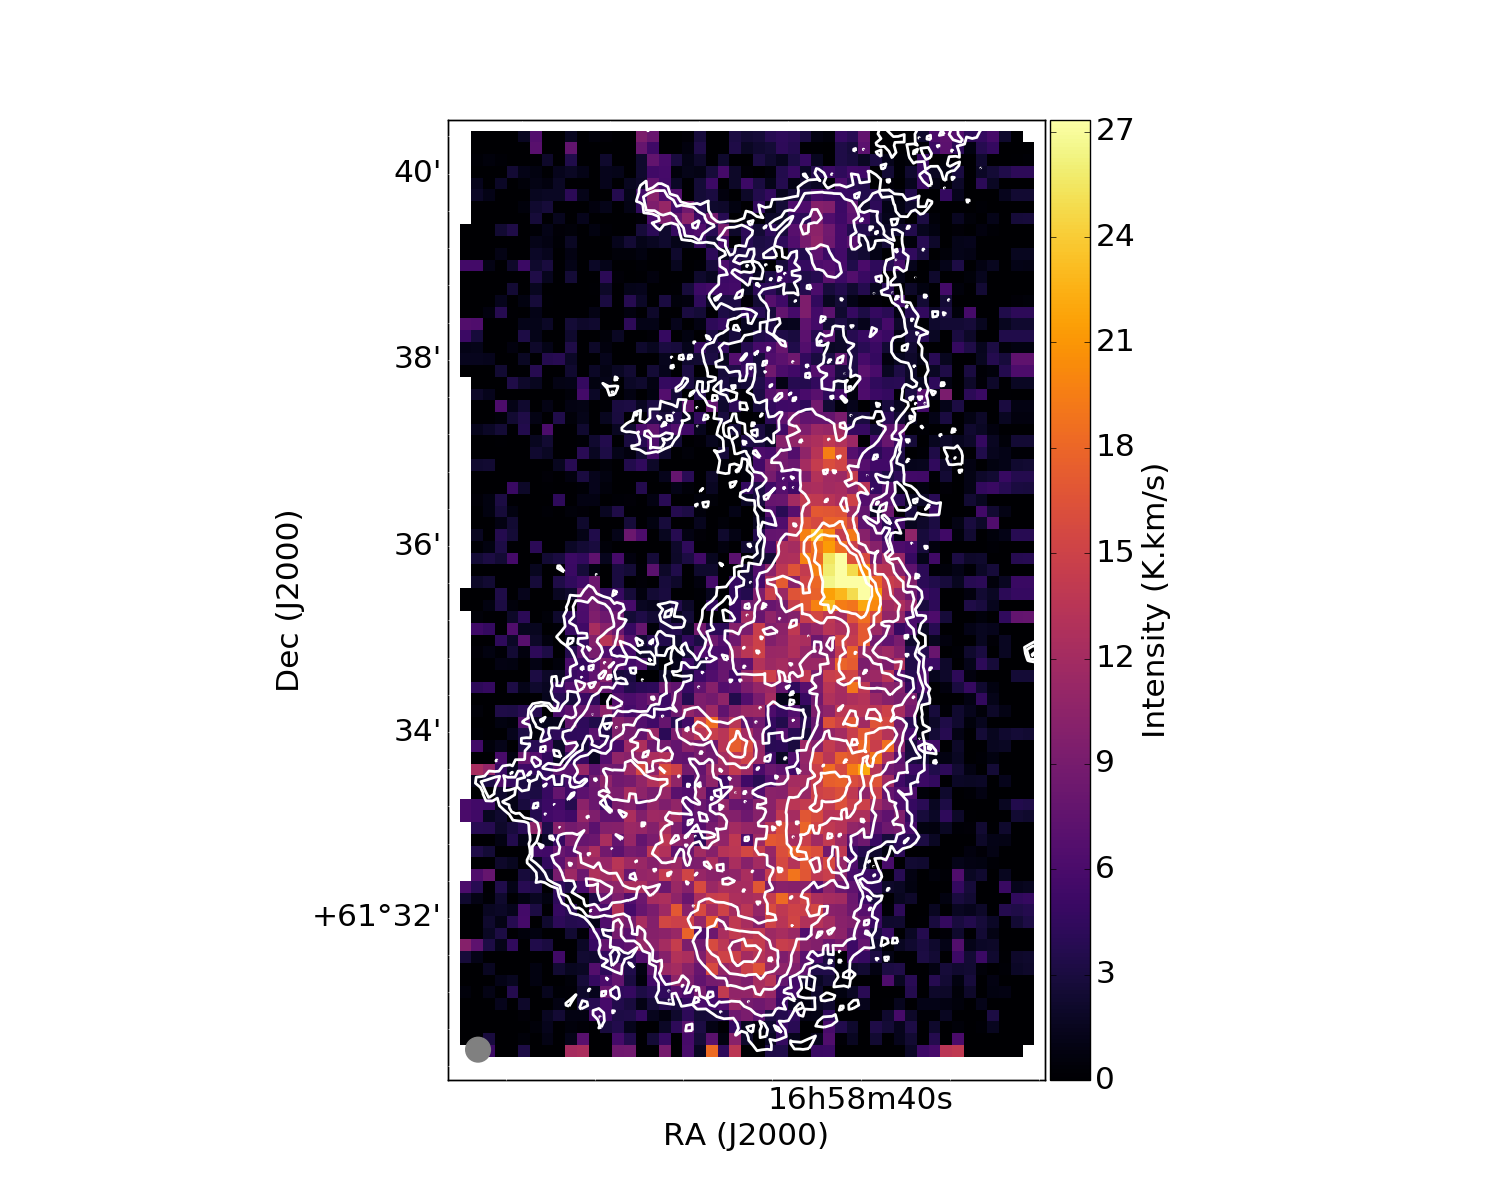
\includegraphics[height=4.5cm,trim=50 40 50 40,clip=true]{Figures/Draco4_stack.png} \\
  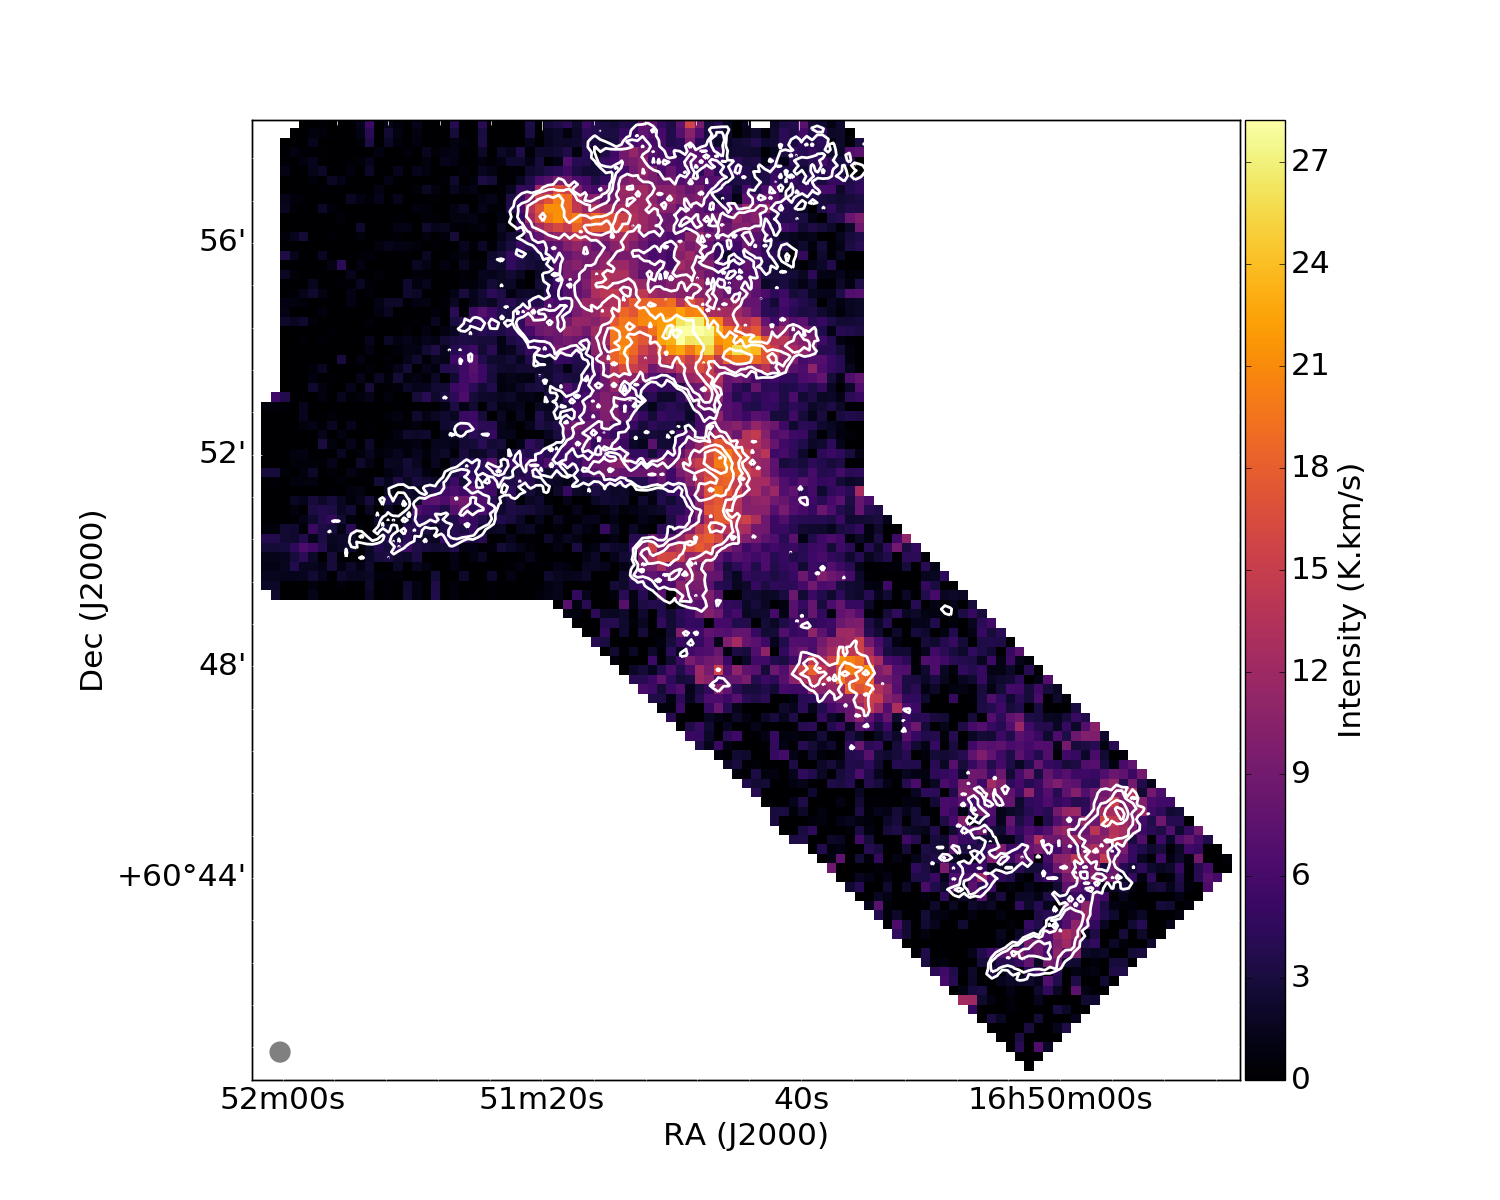
\includegraphics[height=4.5cm,trim=50 40 50 40,clip=true]{Figures/Draco2+9_stack.png}
  \hspace{3mm}
  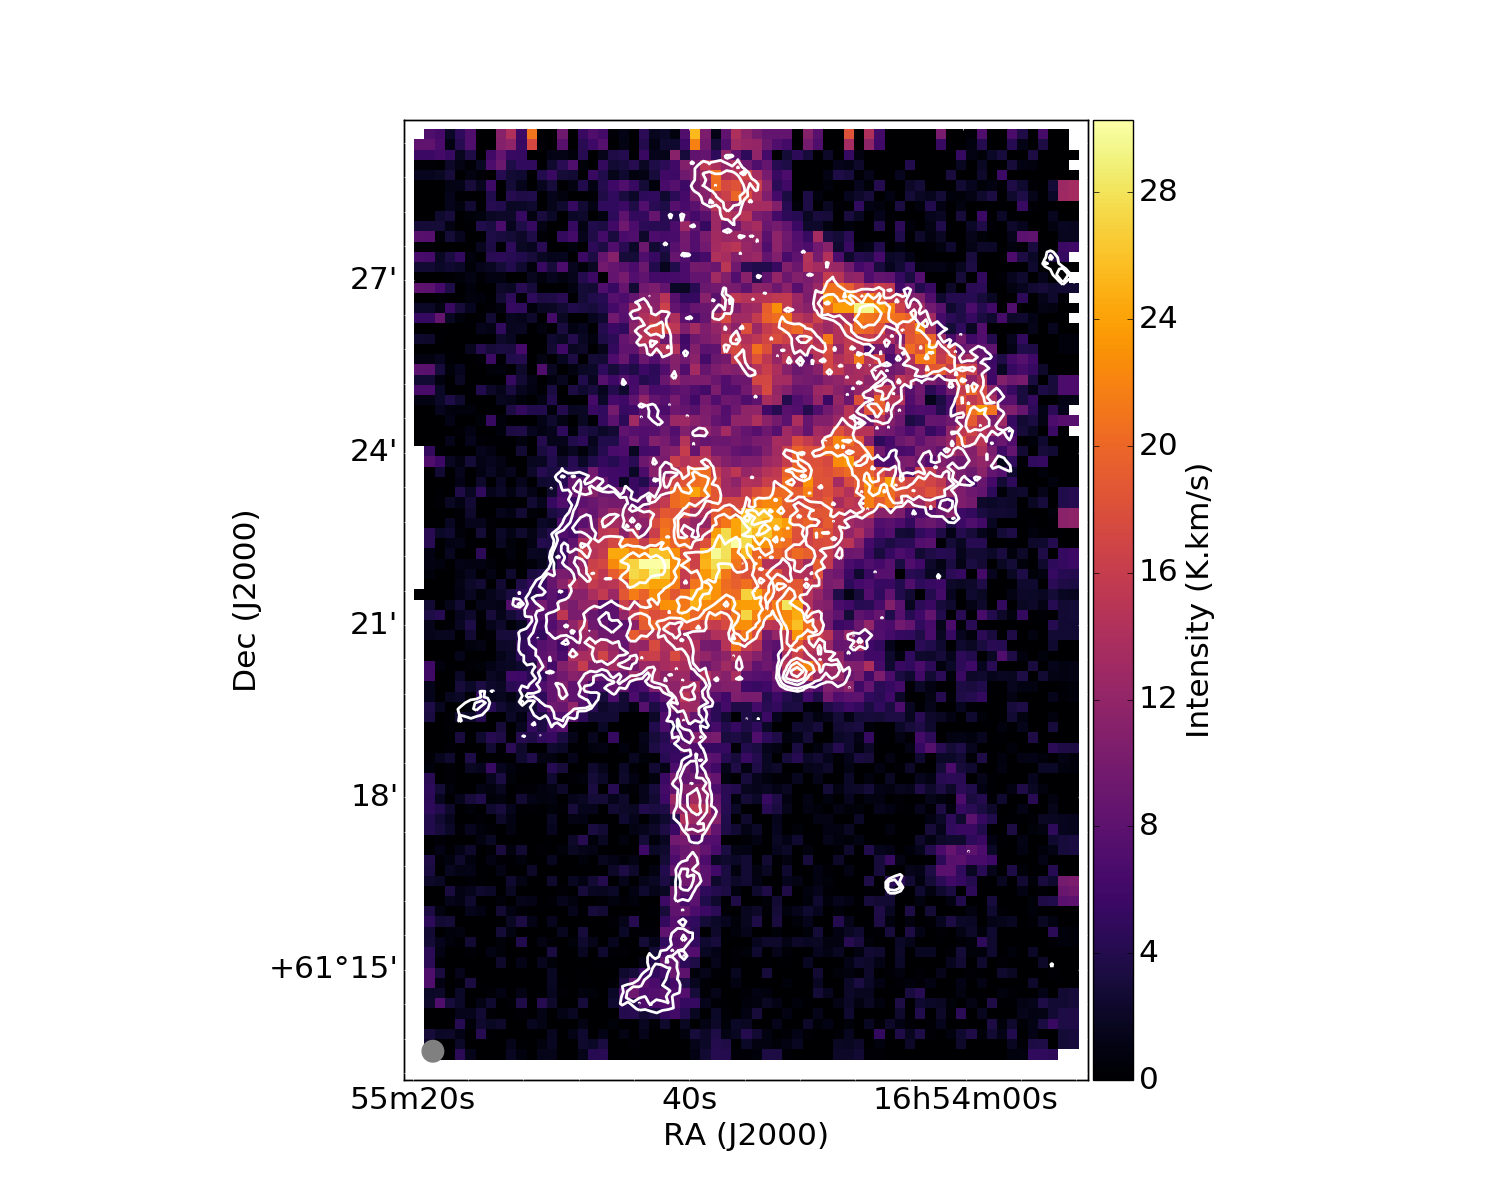
\includegraphics[height=4.5cm,trim=50 40 50 40,clip=true]{Figures/Draco5_stack.png} \\
  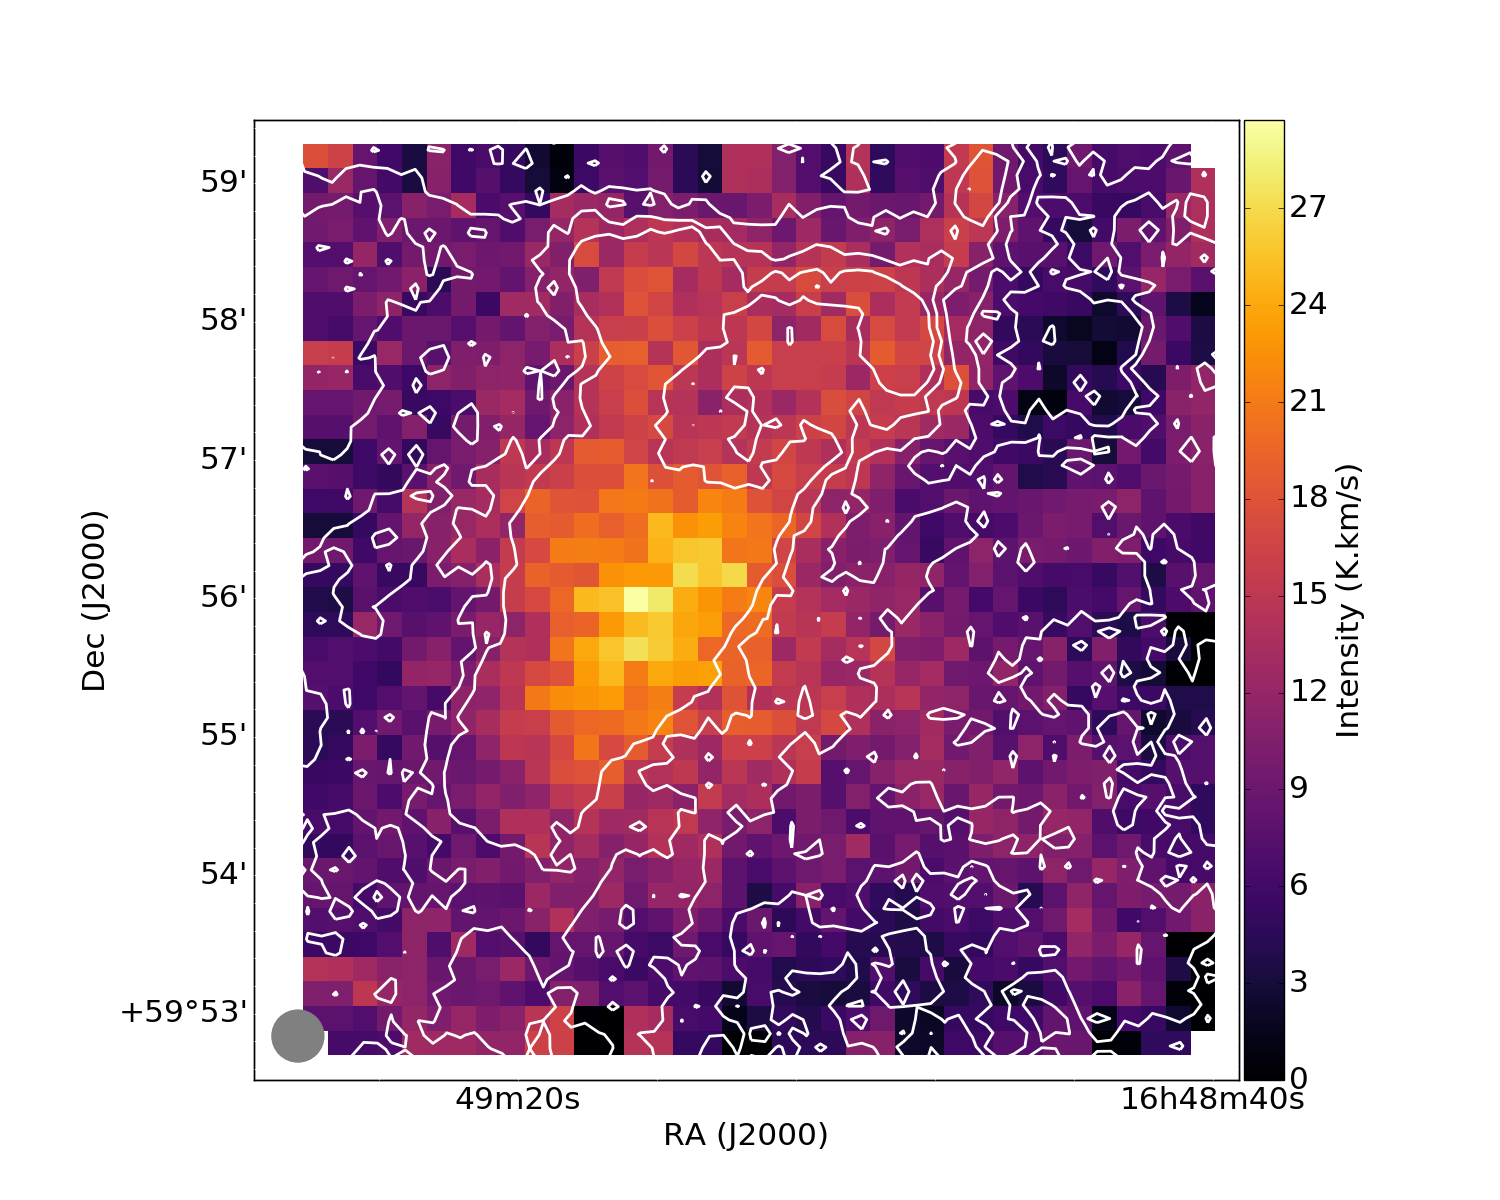
\includegraphics[height=4.5cm,trim=50 40 50 40,clip=true]{Figures/Draco3_stack.png}
  \hspace{3mm}
  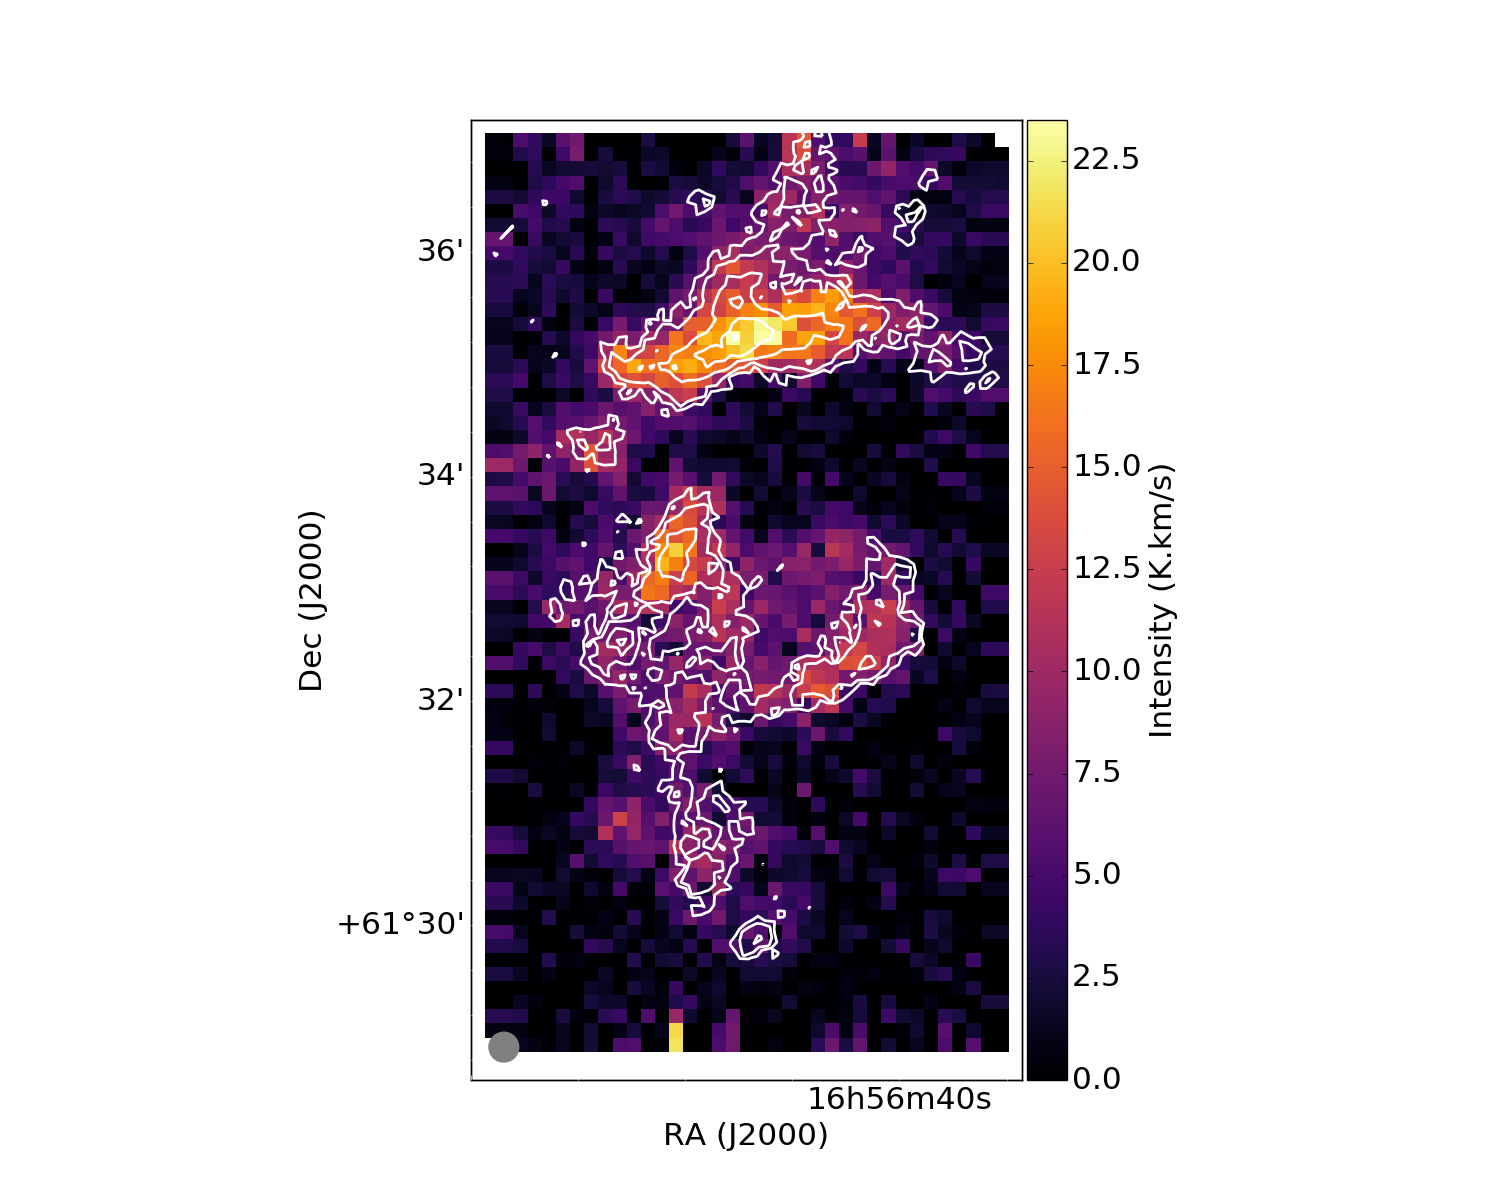
\includegraphics[height=4.5cm,trim=50 40 50 40,clip=true]{Figures/Draco6_stack.png} \\
  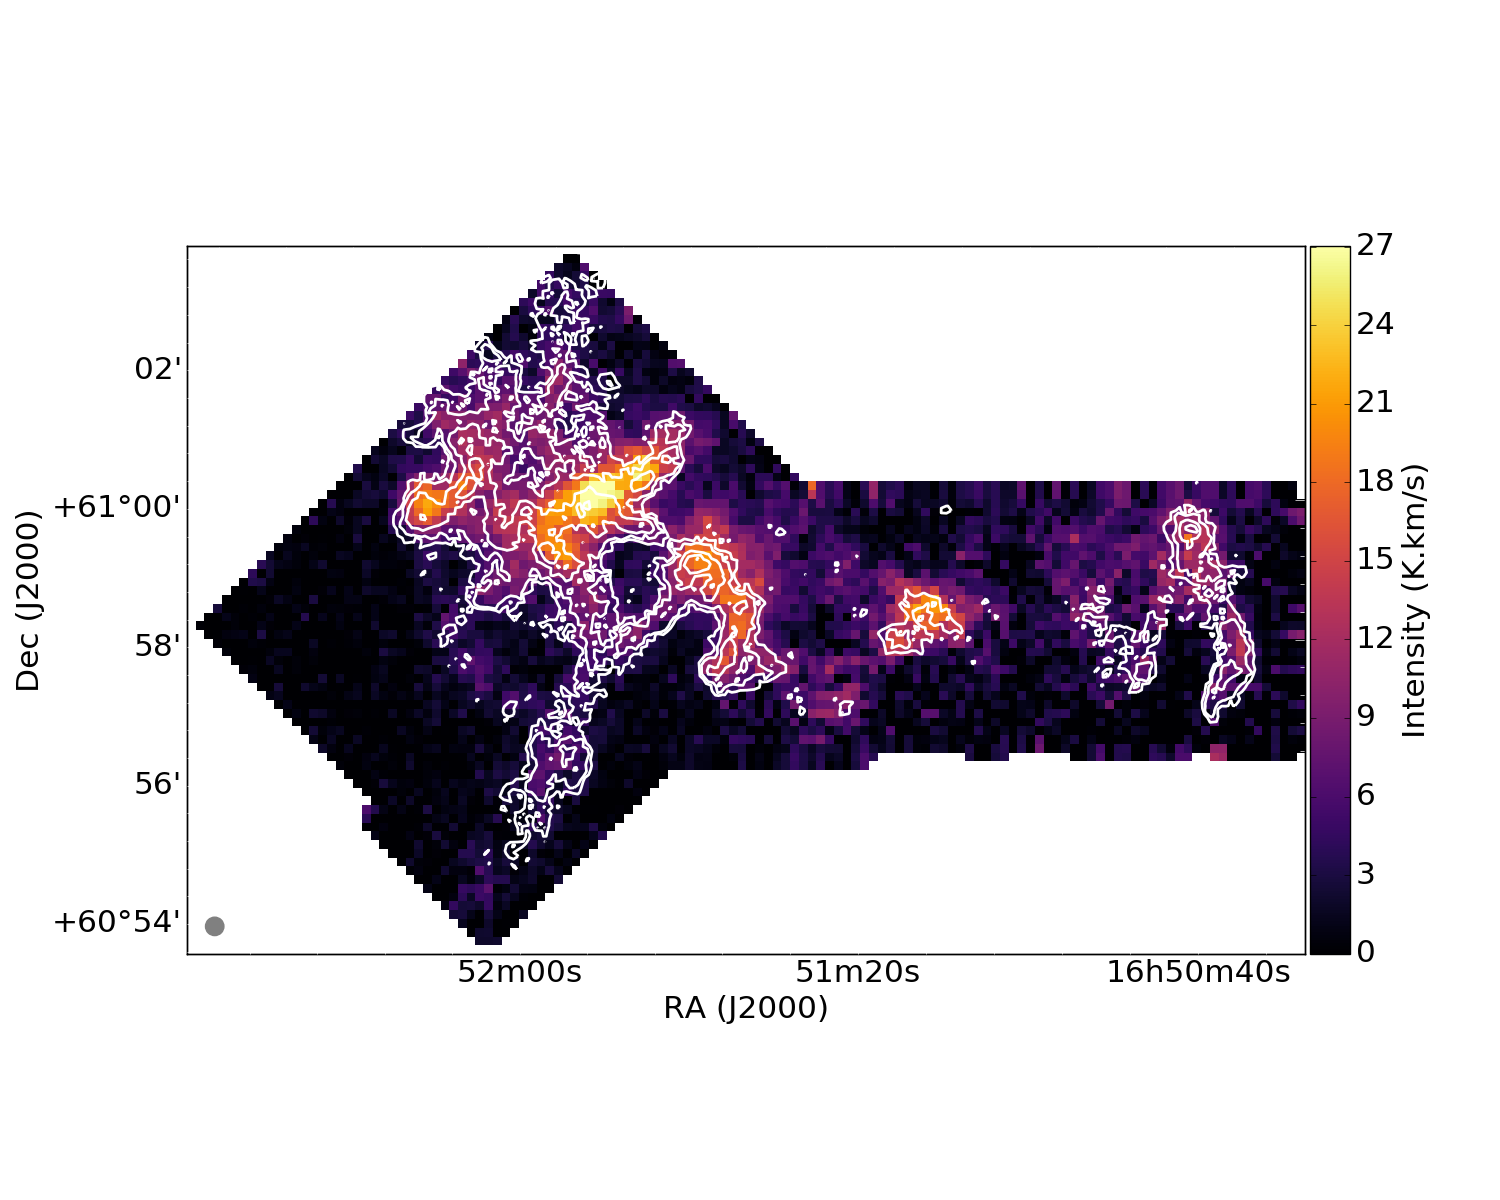
\includegraphics[height=4.5cm,trim=50 40 50 40,clip=true]{Figures/Draco2+9_rot_stack.png}
  \caption{\label{Draco_CO10} Intensity maps in $K.km.s^{-1}$ of the CO(1-0) emission in the different regions observed with the IRAM 30m. The black contours are the dust emission observed at $250\: mu m$ with \emph{Herschel}-SPIRE.}
\end{figure*}

\begin{figure*}[h]
  \centering
  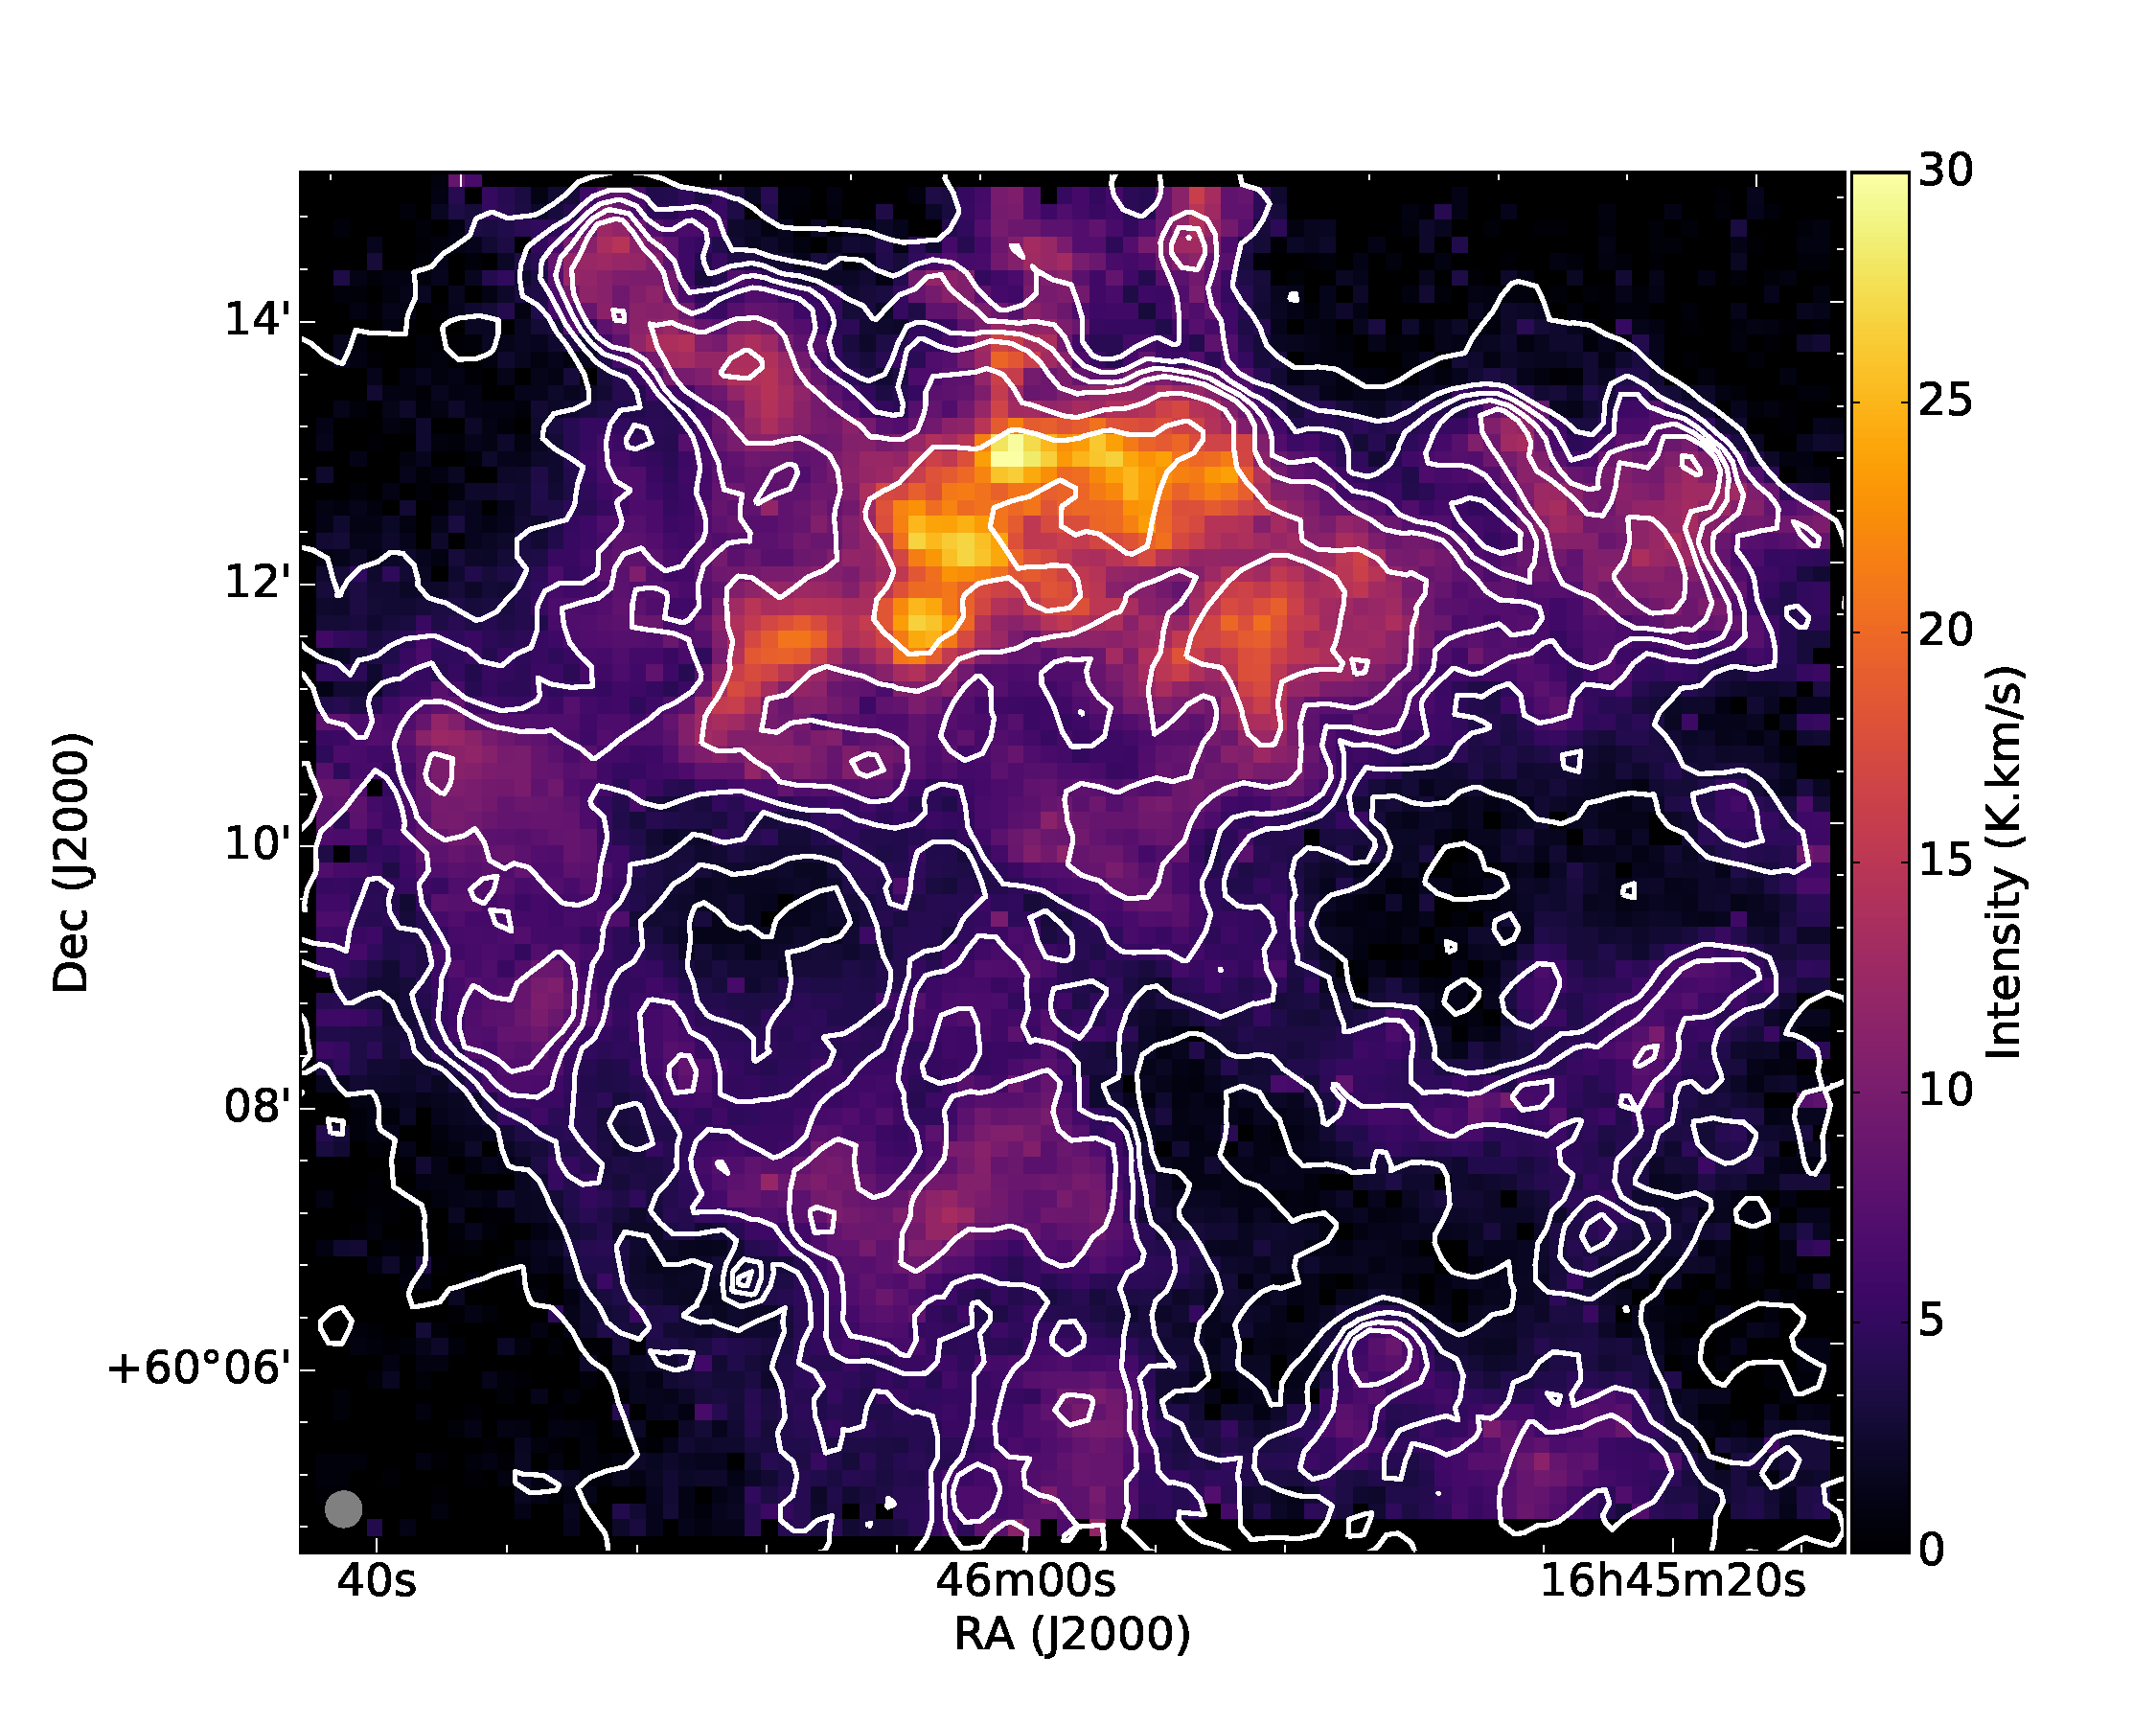
\includegraphics[page=1,height=4.5cm,trim=50 40 50 40,clip=true]{Figures/CO10_intensity.pdf}
  \hspace{3mm}
  \includegraphics[page=4,height=4.5cm,trim=50 40 50 40,clip=true]{Figures/CO10_intensity.pdf} \\
  \includegraphics[page=2,height=4.5cm,trim=50 40 50 40,clip=true]{Figures/CO10_intensity.pdf}
  \hspace{3mm}
  \includegraphics[page=5,height=4.5cm,trim=50 40 50 40,clip=true]{Figures/CO10_intensity.pdf} \\
  \includegraphics[page=3,height=4.5cm,trim=50 40 50 40,clip=true]{Figures/CO10_intensity.pdf}
  \hspace{3mm}
  \includegraphics[page=6,height=4.5cm,trim=50 40 50 40,clip=true]{Figures/CO10_intensity.pdf} \\
  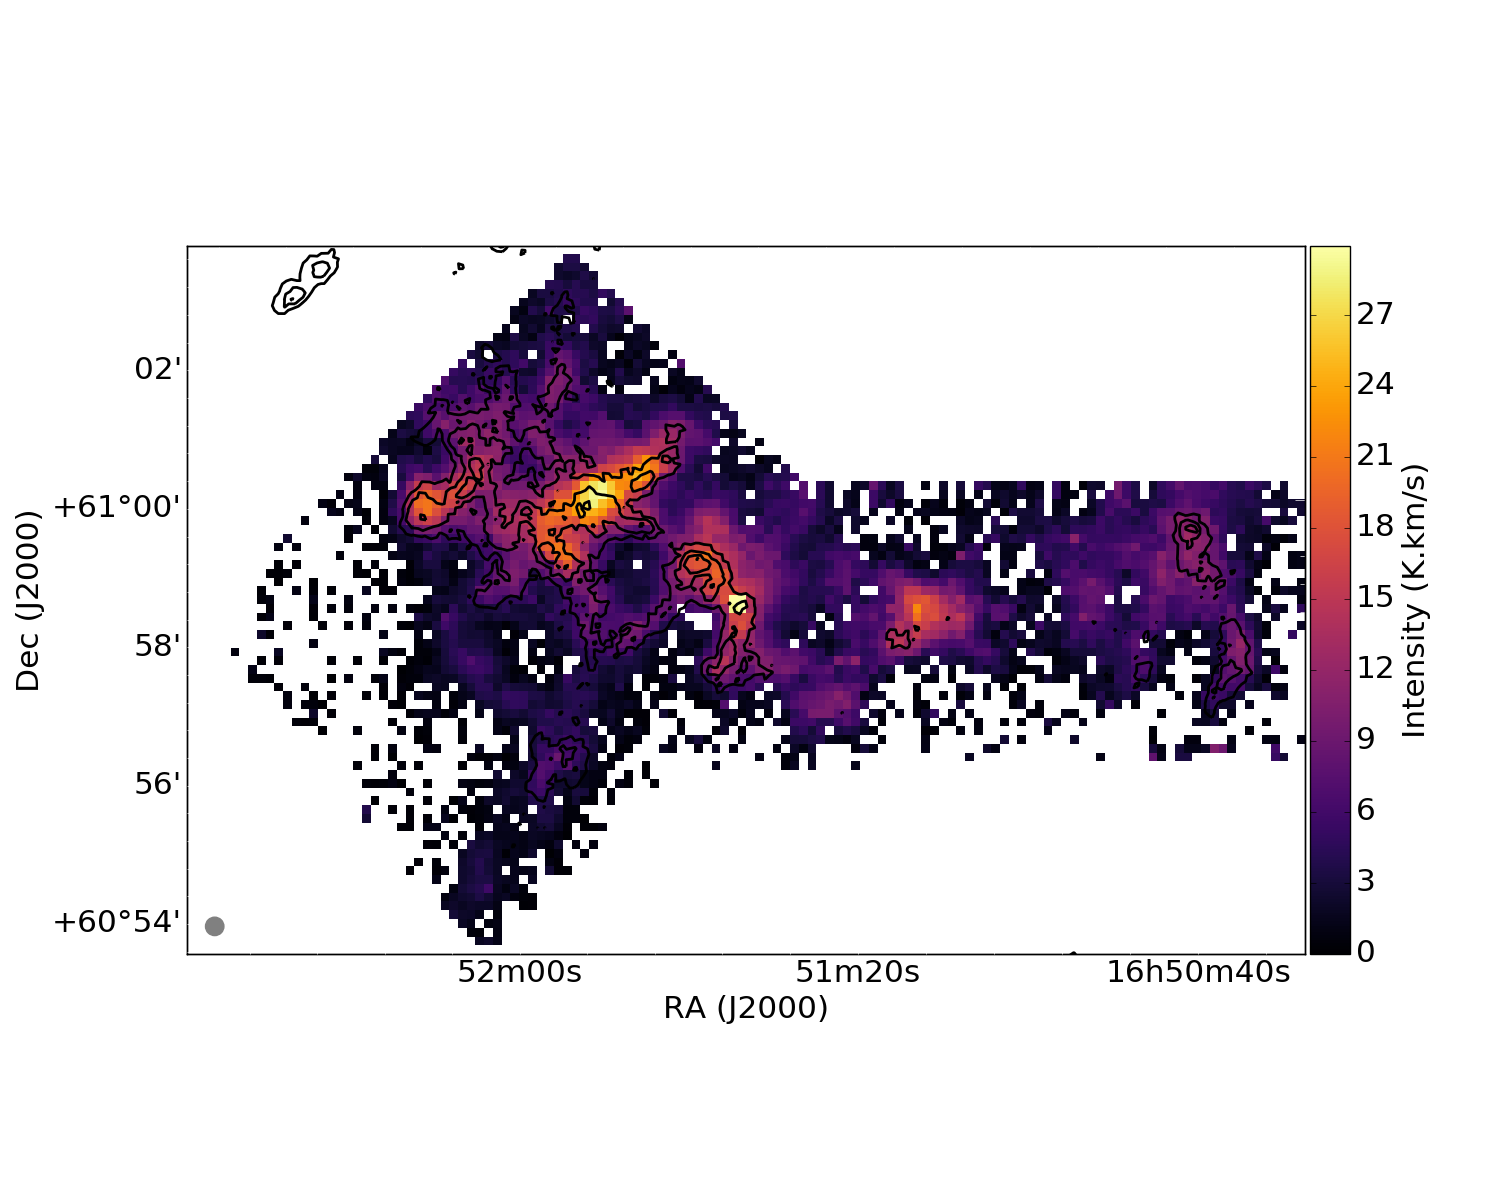
\includegraphics[height=4.5cm,trim=50 40 50 40,clip=true]{Figures/Draco2+9_rot_intensity.png}
  \caption{\label{Draco_CO10} Intensity maps in $K.km.s^{-1}$ of the CO(1-0) emission in the different regions observed with the IRAM 30m. The black contours are the dust emission observed at $250\: mu m$ with \emph{Herschel}-SPIRE.}
\end{figure*}

\begin{figure*}[h]
  \centering
  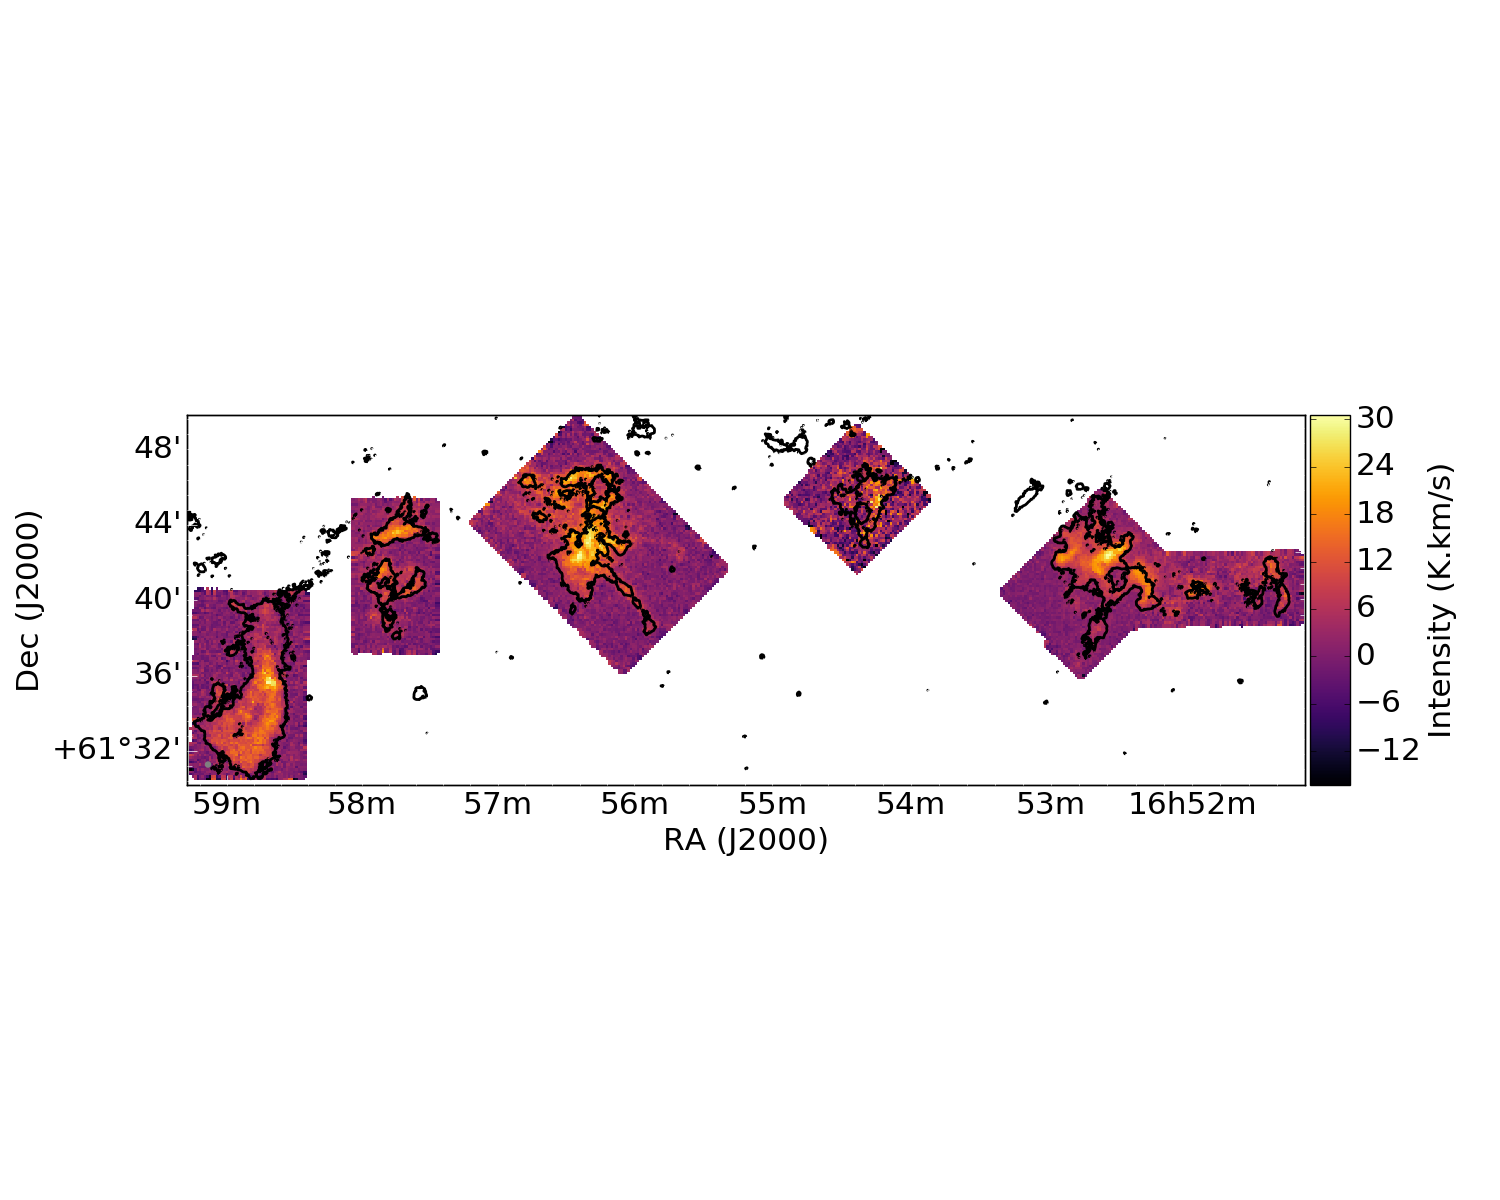
\includegraphics[width=\linewidth,trim=0 250 0 250,clip=true]{Figures/Draco_FRONT_stack.png} \\
  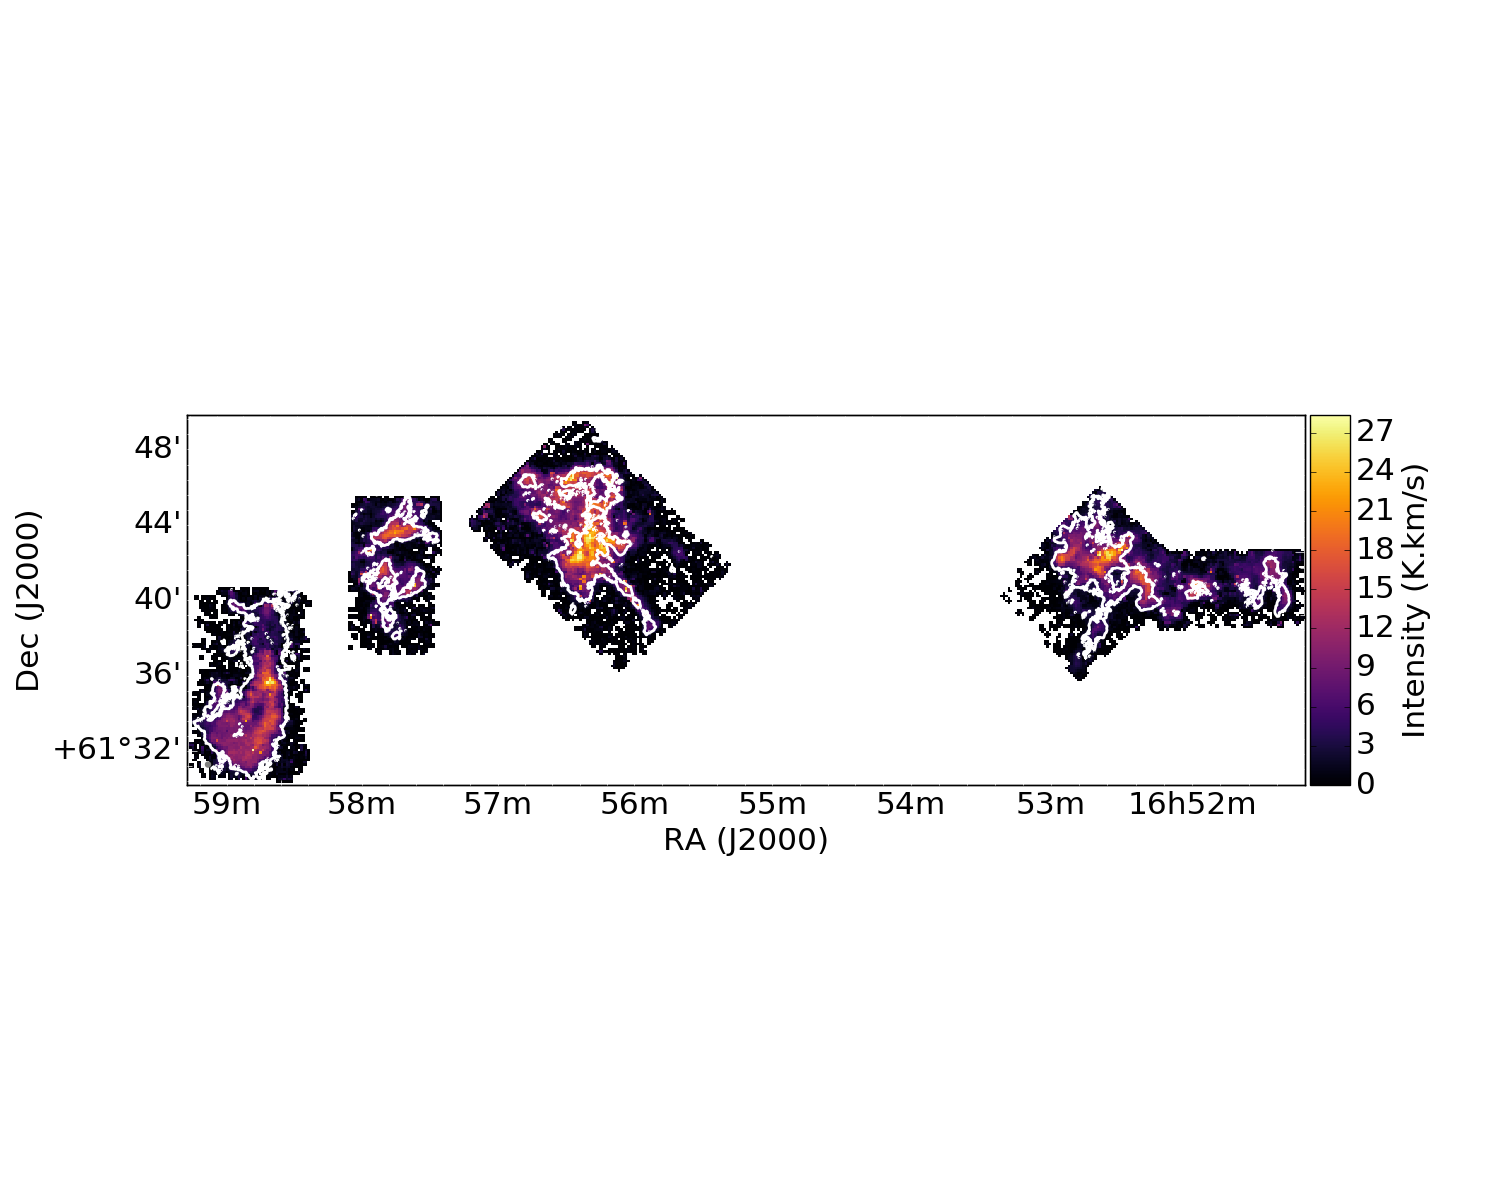
\includegraphics[width=\linewidth,trim=0 250 0 250,clip=true]{Figures/Draco_FRONT_intensity.png}
  \caption{\label{Draco_CO10} Intensity maps in $K.km.s^{-1}$ of the CO(1-0) emission in the different regions observed with the IRAM 30m. The black contours are the dust emission observed at $250\: mu m$ with \emph{Herschel}-SPIRE.}
\end{figure*}

\begin{equation}
  N(H)=2.49\times 10^{20}\, I_{250\: \mu m}
\end{equation}
We smoothed the so-done total column density and the CO intensity maps at the resolution of the DHIGLS $H\rmnum{1}$ map ($1'$). We are now able to determine the $X_{CO}$ factor that is given by:
\begin{equation}
  N(H)-N(H\rmnum{1})=2\times X_{CO}\, I_{CO}
\end{equation}
In Draco1, we found a $X_{CO}$ factor of $(1.97\pm 0.01)\times 10^{20}\: cm^{-1}.(K.km.s^{-1})^{-1}$, typical of what is observed in the Galactic disc\citep{Bolatto_2013}. On the opposite, molecular gas in Draco2 seems to be CO-bright. The plot of $I_{CO}$ vs. $N_{H_2}$ shows two regimes: at $I_{CO}\leq 5\: K.km.s^{-1}$ where $X_{CO}=(1.92\pm 0.03)\times 10^{20}\: cm^{-1}.(K.km.s^{-1})^{-1}$, and at $I_{CO}>5\: K.km.s^{-1}$ with an average value of $(0.55\pm 0.04)\times 10^{20}\: cm^{-1}.(K.km.s^{-1})^{-1}$.
Such values of the $X_{CO}$ factor are a factor of 3-4 times higher to those previously found by \cite{Herbstmeier_1993} and \cite{Moritz_1998}.
%Intercept ($N_{H_2}^0$) is about $6.1-5.9\times 10^{20}\: cm^{-2}$ \textbf{(???; due to optically thin hypothesis \citep{Okamoto_arXiv}?)}.

\begin{table}[h]
  \centering
  \footnotesize
  \caption{\label{table:Xco} Values of the $X_{CO}$ factor estimation.}
  \begin{tabular}{lc}
    \hline \hline
    Region &       $X_{CO}$       \\ \hline 
    Draco1 & $1.98\times 10^{20}$ \\
    Draco2 & $1.16\times 10^{20}$ \\
    Draco3 & $1.94\times 10^{20}$ \\
    Draco4 & $1.70\times 10^{20}$ \\
    Draco5 & $0.77\times 10^{20}$ \\
    Draco6 & $1.22\times 10^{20}$ \\ \hline
  \end{tabular}
\end{table}

\begin{figure*}[h!]
  \centering
  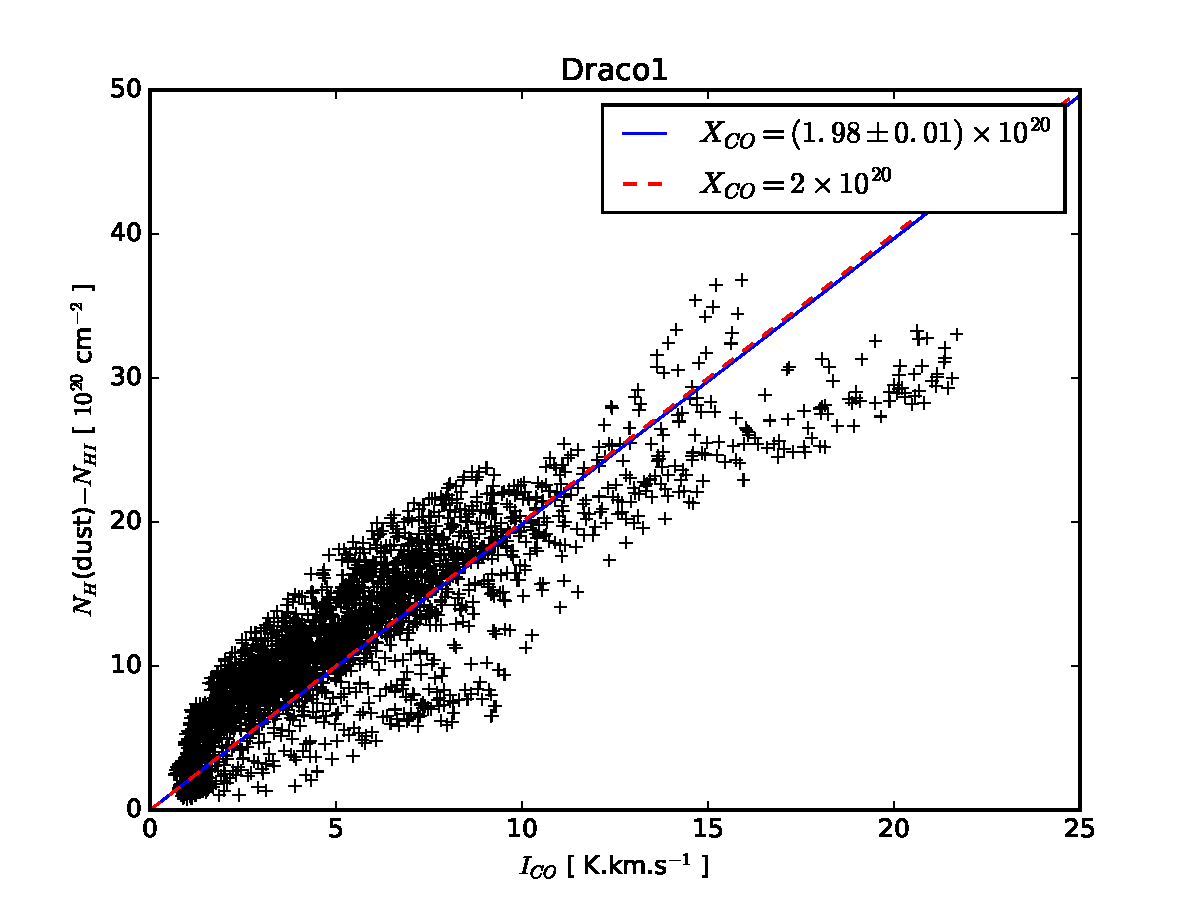
\includegraphics[page=1,width=0.48\linewidth,trim=30 10 50 30,clip=true]{Figures/dust-CO_comparison.pdf}
  \hspace{3mm}
  \includegraphics[page=2,width=0.48\linewidth,trim=30 10 50 30,clip=true]{Figures/dust-CO_comparison.pdf}
  \caption{\label{Xco} Correlation between the total column density derived from dust emission and the CO integrated intensity in Draco1 (\emph{left}) and Draco2 (\emph{right}). The slope of the best fitting model (blue line) gives the value of the $X_{CO}$ factor. The red dashed line corresponds to the value found by \cite{Moritz_1998}.}
\end{figure*}


\subsubsection{CO line ratios}

We smoothed the CO(2-1) map to the resolution of the CO(1-0) map in order to look at the CO(2-1)/CO(1-0) ratio. The line ratio is rather spatially uniform, with values of $0.67\pm 0.11$ in Draco1 and $0.73\pm 0.11$ in Draco2. Such values is typical to what is found for molecular clouds in the Milky Way and nearby galaxies \textbf{(ref!)}. \textbf{Variations in the CO(2-1)/CO(1-0) line ratio?}

\begin{table}[h]
  \centering
  \footnotesize
  \caption{Average CO(2-1)/CO(1-0) intensity line ratio}
  \begin{tabular}{lcccccc}
    \hline \hline
    Region & $I_{CO21}/I_{CO10}$ \\ \hline
    Draco1 &   $0.67\pm 0.11$    \\
    Draco2 &   $0.75\pm 0.14$    \\
    Draco3 &   $0.73\pm 0.07$    \\
    Draco4 &   $0.75\pm 0.12$    \\
    Draco5 &   $0.84\pm 0.12$    \\
    Draco6 &   $0.70\pm 0.11$    \\ \hline
  \end{tabular}
\end{table}

\begin{figure*}[h!]
  \centering
  \includegraphics[page=2,height=7.3cm,trim=60 30 90 75,clip=true]{Figures/Draco1_CO21-CO10.pdf}
  \hspace{3mm}
  \includegraphics[page=2,height=7.3cm,trim=70 30 90 75,clip=true]{Figures/Draco2_CO21-CO10.pdf}
  \caption{\label{ratio} Histogram of the line ratio CO(2-1)/CO(1-0) in Draco1 (\emph{left}) and Draco2 (\emph{right}). The best fitting Gaussian indicates a line ratio of the order to what is commonly found in the interstellar medium (about 0.7; \textbf{ref!}). \textbf{Is it relevant to show these histograms?}}
\end{figure*}

\textbf{Use gaussian decomposition to separate the different component? Diffuse vs. dense? Histogram of the sigma?}
%__________________________________________________________________________________________________________________________________
\subsubsection{CO-H\rmnum{1} comparison}

   We now aim to compare the dynamics of the CO and H\rmnum{1} emission. First, we compared the velocity of the CO(1-0) and CO(2-1). As expected both CO lines have rather the same velocity, with a relative difference of $2.4-3.3\%$. We then compared the velocity maps of the CO(1-0) and H\rmnum{1} emission at the resolution of the DHIGLS data. The CO and H\rmnum{1} velocity are rather similar, indicating that the atomic and molecular gas are well mixed in the two regions observed in CO with the IRAM 30m.

   In a second time, we looked at the position-velocity (PV) diagrams of both H\rmnum{1} and CO(1-0) emission at the shock interface in Draco2. The velocity map of CO shows a velocity gradient along a "slit" oriented at 45\degree, the orientation we chose to compute the PV diagrams. To do so, we decreased the spatial and spectral resolution of the CO data to those of the HI data ($1'$ in space and $0.8\: km.s^{-1}$ in velocity). For both emission, we focused on the region where CO has been observed ($300''\times 420''$). We finally stacked all the pixels in the direction orthogonal to the "slit". The resulting PV diagrams are shown in figure \ref{PV-diag}.

\begin{figure*}[h!]
  \centering
  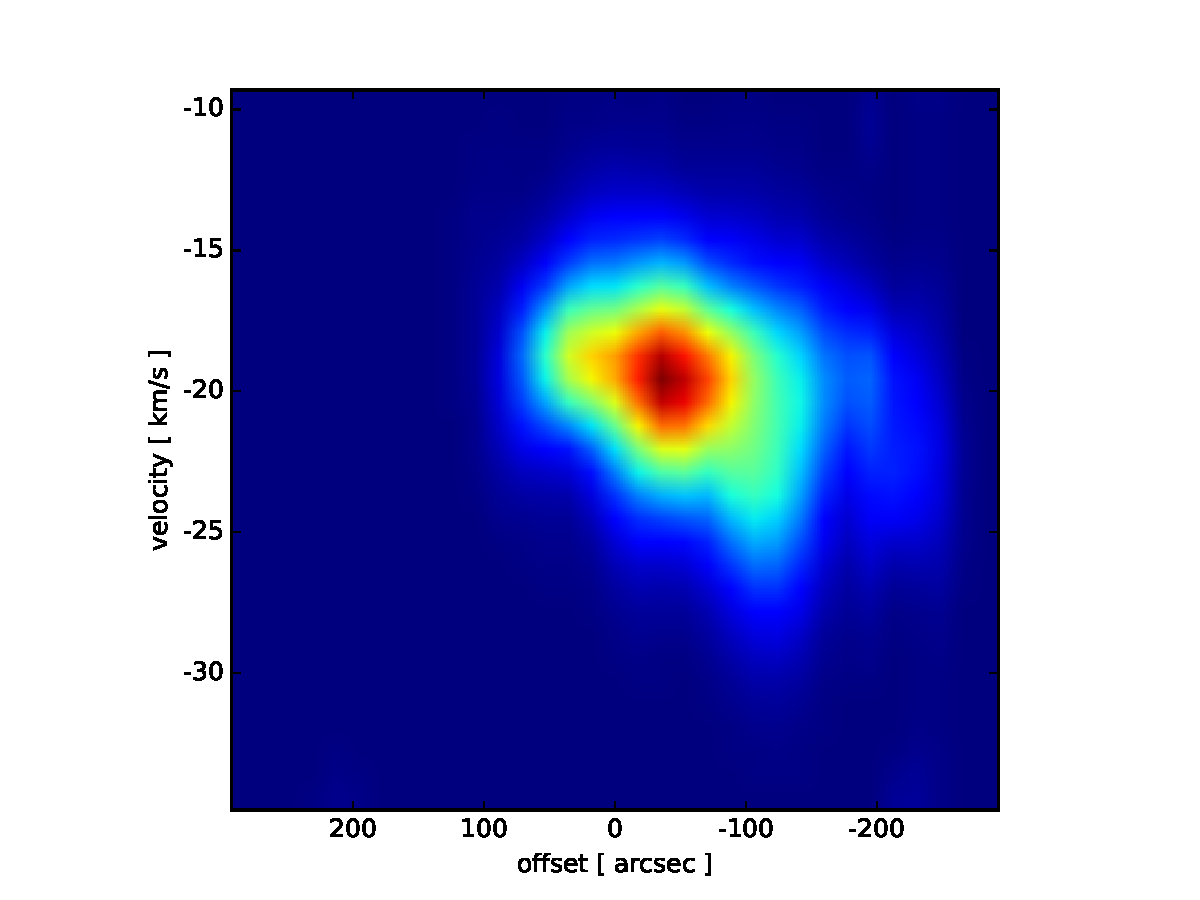
\includegraphics[width=0.48\linewidth,trim=70 10 95 40,clip=true]{Figures/PV_diagram_HI.pdf}
  \hspace{3mm}
  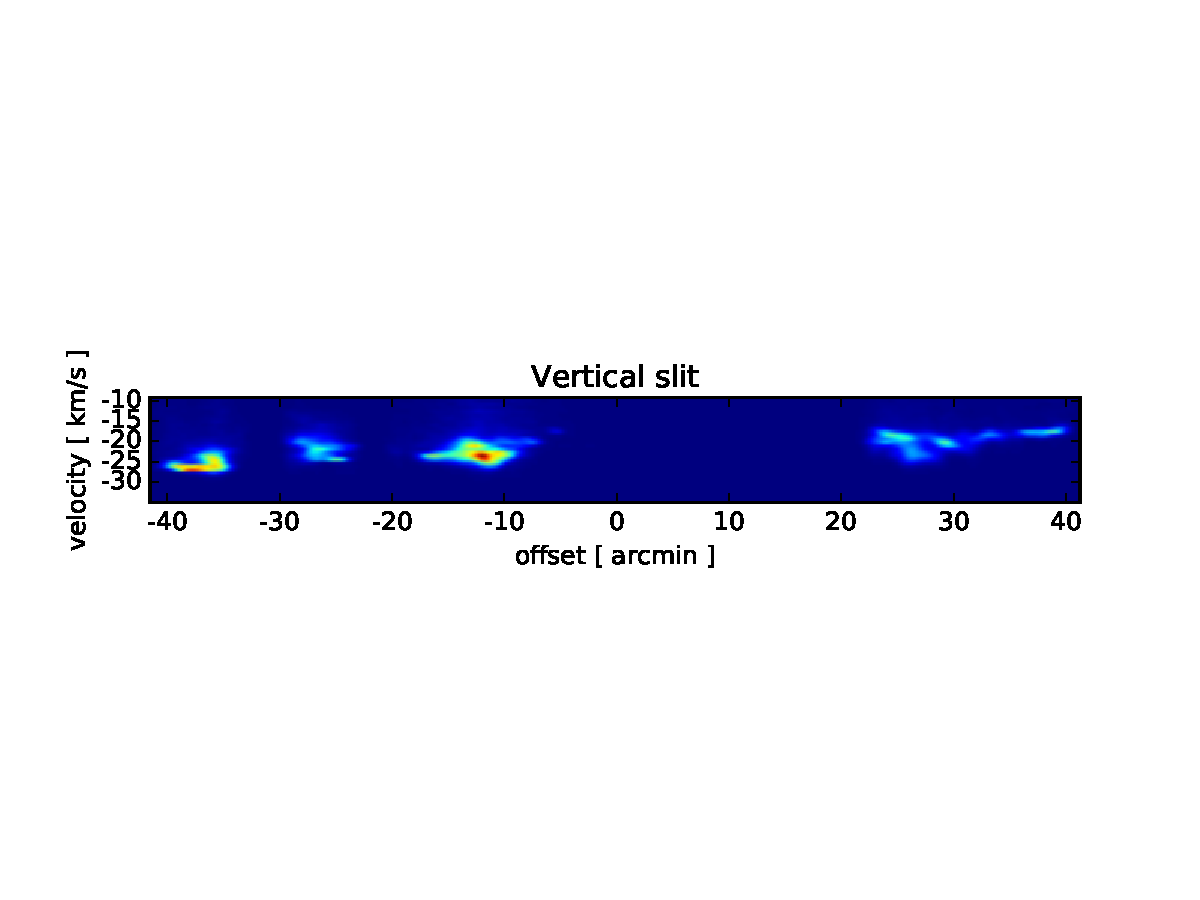
\includegraphics[width=0.48\linewidth,trim=70 10 95 40,clip=true]{Figures/PV_diagram_CO.pdf}
  \caption{\label{PV-diag} Position-velocity diagrams of the H\rmnum{1} (\emph{left}) and CO (\emph{right}) in Draco2. The PV diagrams are centred in $\alpha=16^h 51^m 13.3^s$, $\delta=+$60:55:23.7 over a slit oriented at 45\degree with a width of $8.5'$, to include all the region observed in CO. They were computed at $1'$ and $0.8\: km.s^{-1}$ resolution.}
\end{figure*}


\subsection{Molecular gas fraction}

\textbf{Discuss the spatial distribution of CO compare to H\rmnum{1} (figure \ref{DRAO-CO})}

\begin{figure}[h!]
  \centering
  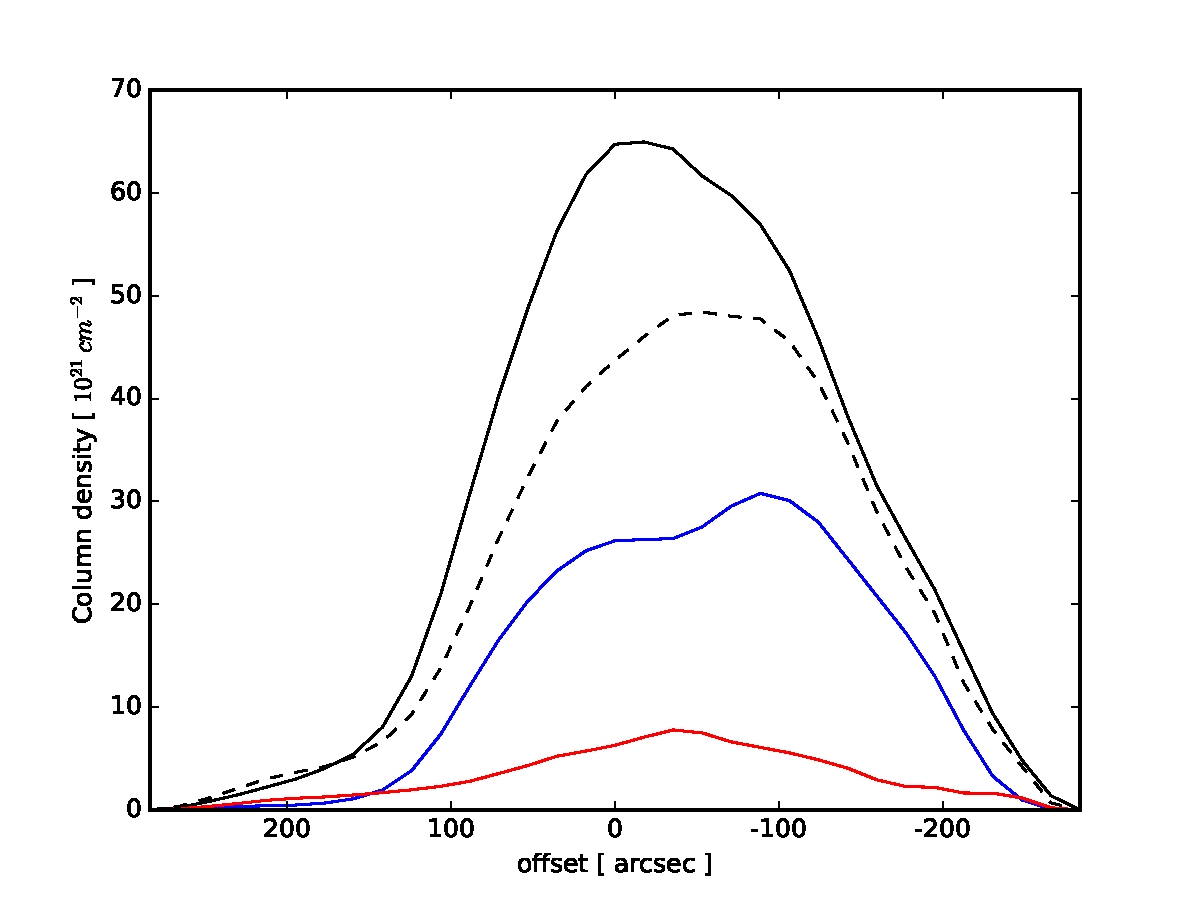
\includegraphics[width=\linewidth,trim=30 10 55 35,clip=true]{Figures/Column_density_profiles.pdf}
  \caption{\label{Col_density} Density profiles of the total column density $N_H$ (black line), derived from the \emph{Herschel}-SPIRE $250\: \mu m$ emission, the atomic column density $N_{H\rmnum{1}}$ (red line) and the molecular column density $N_{H_2}$ (blue line), derived from the CO emission, along a "slit" oriented at 45\degree. The slit width is $8.5'$, to include all the region observed in CO.}
\end{figure}

\begin{figure*}[h!]
  \centering
  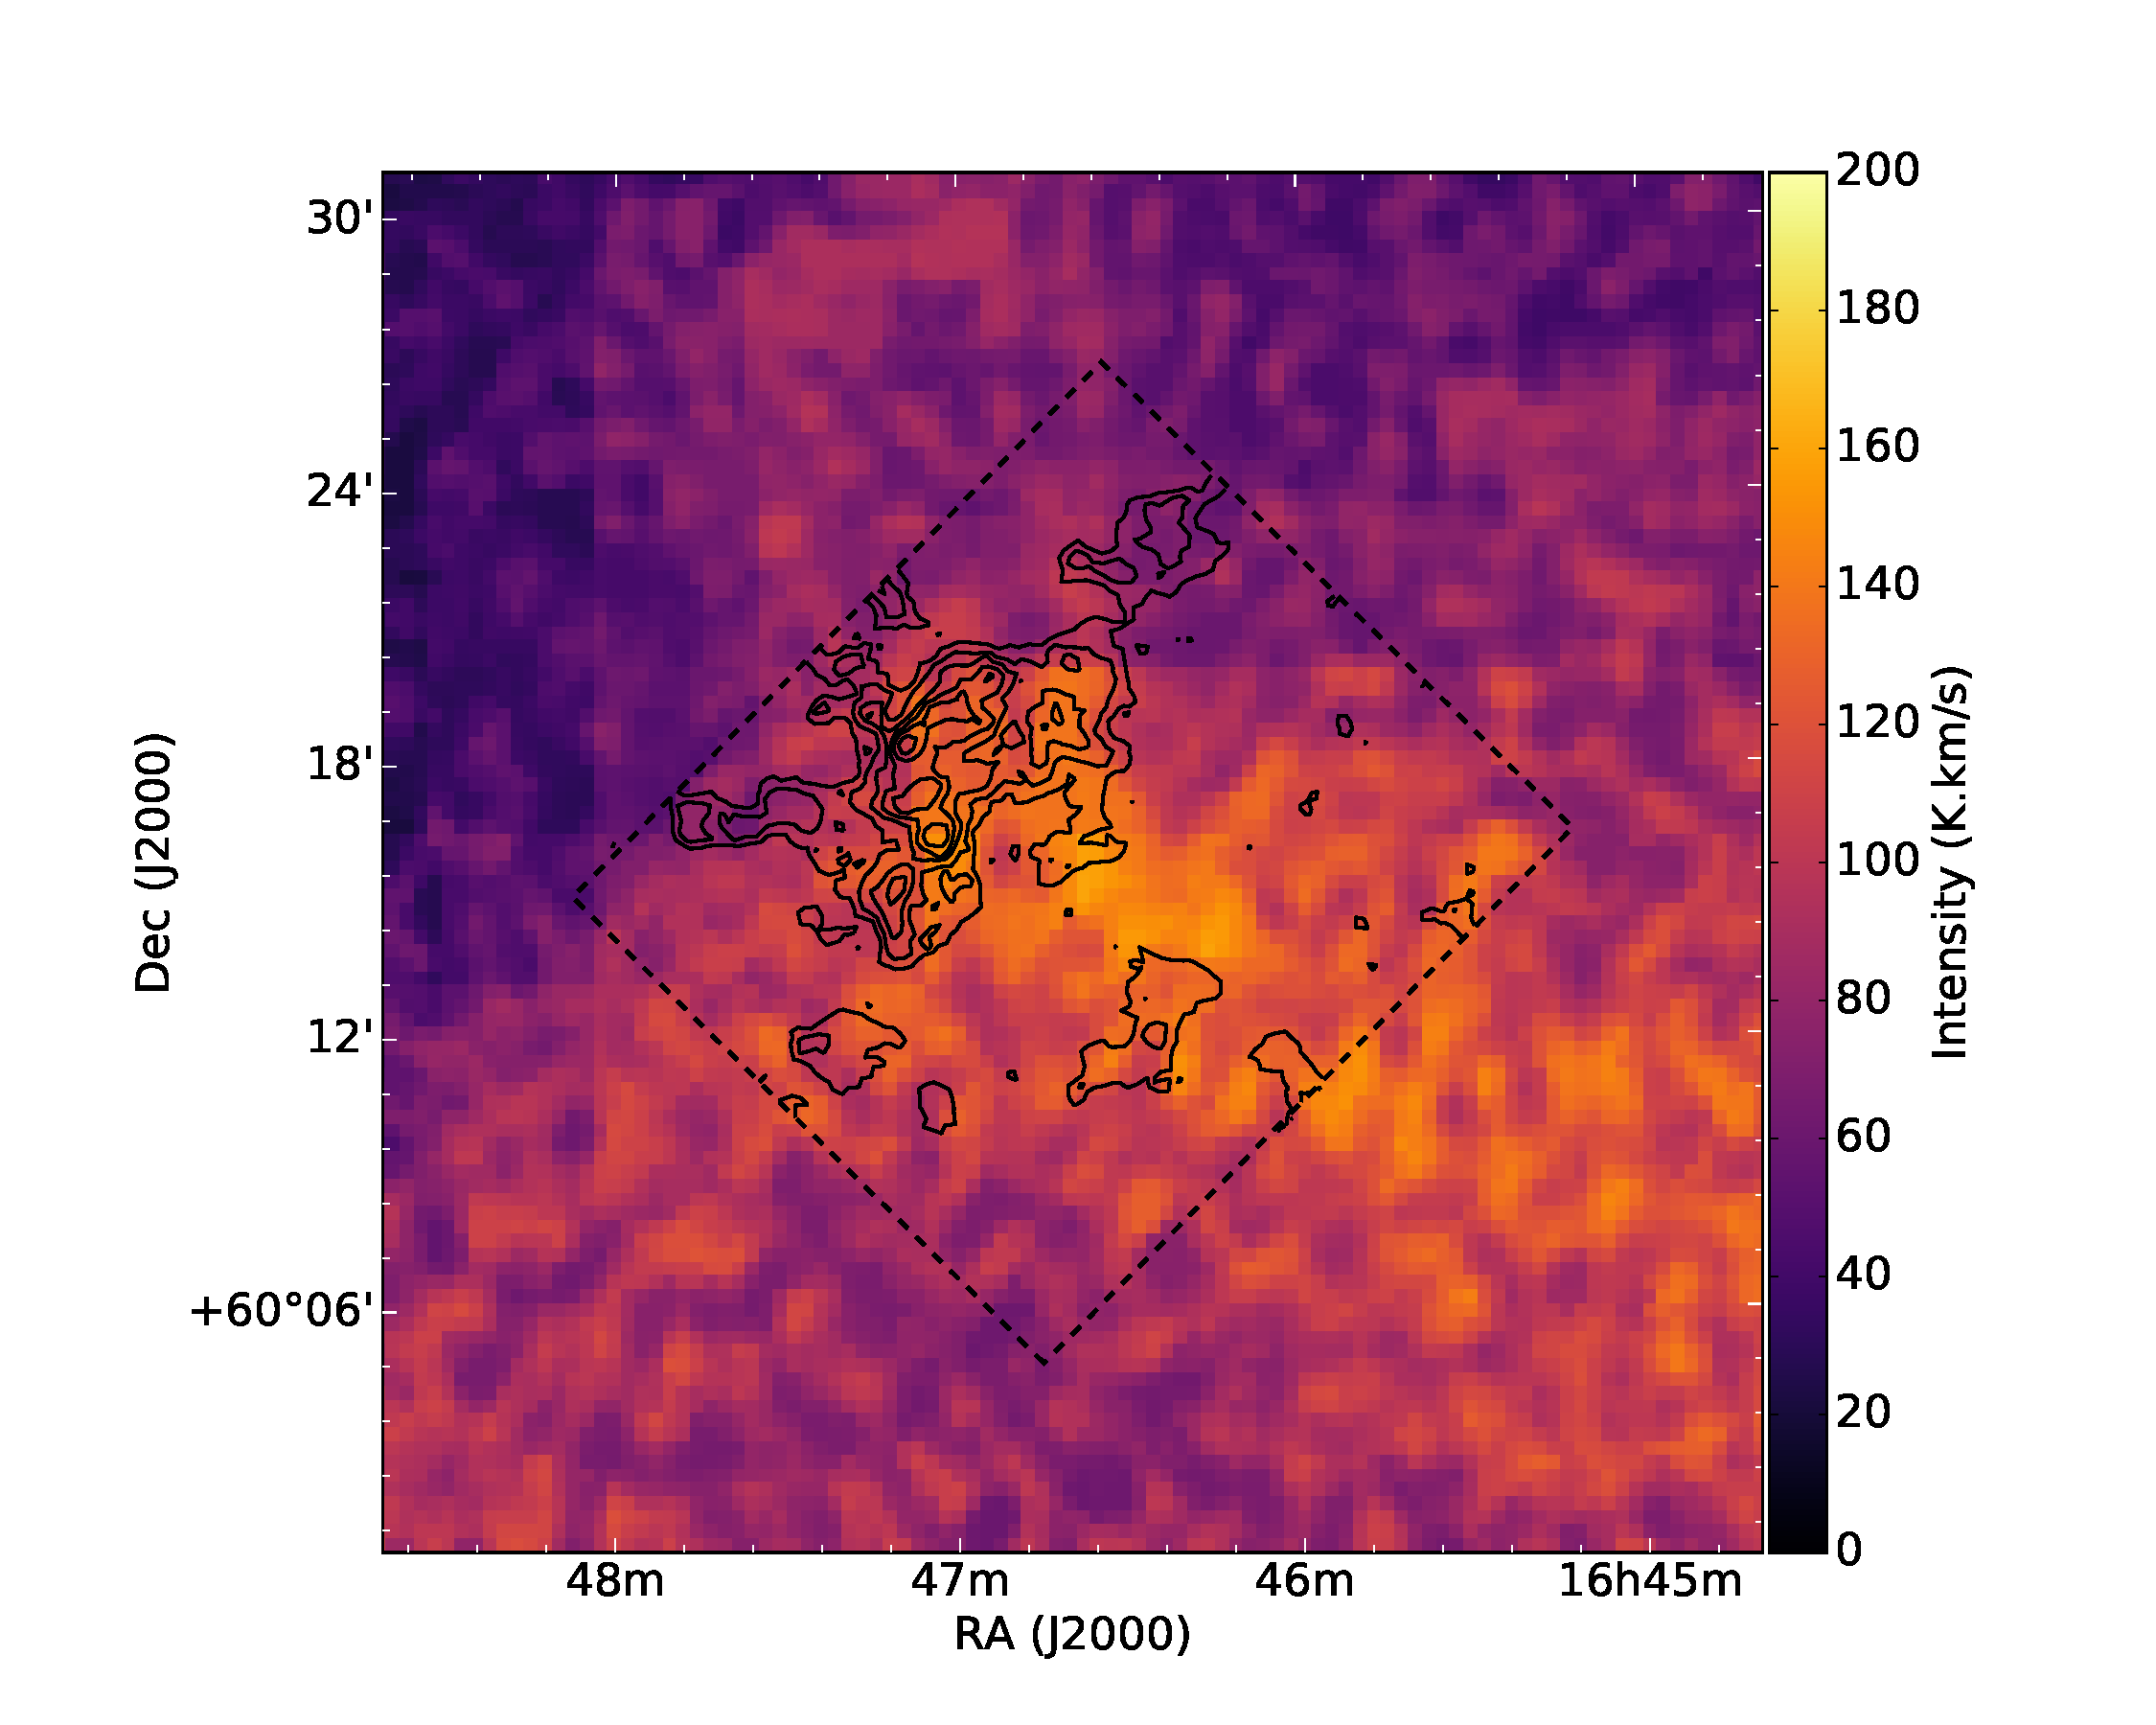
\includegraphics[page=1,width=0.48\linewidth,trim=65 35 115 75,clip=true]{Figures/HI-CO.pdf}
  \hspace{3mm}
  \includegraphics[page=2,width=0.48\linewidth,trim=65 35 115 75,clip=true]{Figures/HI-CO.pdf}
  \caption{\label{DRAO-CO} Map of the H\rmnum{1} emission from DHIGLS, smoothed at a resolution of $1.7'$. The black contours show the CO(1-0) emission observed with the IRAM 30m telescope in the region represented by the dashed boxes. H\rmnum{1} and CO seem to be slightly shifted in projection.}
\end{figure*}

   We used the CO(1-0) and H\rmnum{1} intensity maps to derive the ratio between the molecular and atomic column density. We smoothed the CO maps at the resolution of the DHIGLS map ($1'$). We found a ratio $N(H_2)/N(H\rmnum{1},CNM)$ of $4.0\pm 4.5$ in Draco1 and $2.4\pm 2.0$ in Draco2

\textbf{Estimate the mass of molecular gas produced during the shock?}

\section{Discussion}
\label{sec:discussion}

   \subsection{Mach number an temperature}

\begin{eqnarray}
  \sigma_{H\rmnum{1}}^2 &=& \sigma_{turb}^2+\frac{k T_{H\rmnum{1}}}{\mu_{H\rmnum{1}} m_H} \\
  \sigma_{CO}^2         &=& \sigma_{turb}^2+\frac{k T_{CO}}{\mu_{CO} m_H}
\end{eqnarray}

\subsection{Statistical properties of turbulence}
\textit{VCS (Lazarian et al.)?}

%
%
%   \subsection{A model to compute velocity spectra}
%   \label{sec:model}
%
%   In order to interpret the kinematics of our CO data, we used a simple analytical model which computes the velocity spectrum from the rotation velocity profile of the galaxy \citep{Wiklind_1997}. The rotation velocity profile is determined from the stellar mass distribution, assuming it follows a Plumer distribution.
%
%   The gas distribution was assumed to be axisymmetric of surface density $n(r)$ in a disc with negligible thickness. For each velocity dv, the code calculates the density contained in the isovelocity (equation \ref{eq:dndv}). The velocity spectrum corresponds to the histogram of the velocities. To take into account the gas dispersion, the computed spectrum was then convolved with a gaussian of standard $\sigma=10\: km.s^{-1}$.
%\begin{equation} \label{eq:dndv}
%  \frac{dN}{dv}(v)=\int \frac{n(r)\, rdr}{v_{rot}(r)\sin i \cbra{1-\frac{v}{v_{rot}(r)\sin i}}^2}
%\end{equation}
%
%   We wanted to study the concentration of gas in the galaxy, and determine if the gas is distributed in a disc or a ring. The disc was modelled with a Toomre disc of order 2: $n(r)=n_0\cbra{1+\frac{r^2}{d^2}}^{-5/2}$ \citep{Toomre_1964}. A ring is the difference between two Toomre discs (see sketch in figure \ref{sketch_ring}).
%
%\begin{figure}[h]
%  \centering
%  \includegraphics[width=0.49\linewidth]{/home/qsalome/3C285/Pictures/Sketch_ring.png}
%  \includegraphics[width=0.49\linewidth]{/home/qsalome/3C285/Pictures/Density_profile.png}
%  \caption{\label{sketch_ring} \emph{Left:} Sketch of a ring with the characteristic distances $d_1$ and $d_2$. \emph{Right:} Surface density profile as derived by the model for a Toomre ring of mass $1.03\times 10^{10}\: M_\odot$ with $d_1=0.9\: kpc$ and $d_2=0.5\: kpc$. The vertical blue line represents the size of the CO(2-1) beam for 3C 285.}
%\end{figure}
%
%   We ran grids of model, varying the distances $d_1$ and $d_2$. $d_1$ varies from a few hundred parsecs to 10 kpc, and $d_2$ varies from 0 to a few tens parsecs below $d_1$ ($d_2=0$ corresponds to a disc). Both $d_1$ and $d_2$ have influence on the morphology of gas. For small values of $d_1$, the gas is distributed in a narrow dense ring, whereas for larger distances, the ring is broad with broadness of a few kiloparsecs. In addition, for inner radii larger than $\sim 2\: kpc$, the gas ring extends far enough to be slightly resolved by the IRAM 30m telescope. \\
%The inclination angle will also influence the spectra characteristics. As the radial velocity is proportional to the sine of the angle, the peaks go closer to each other as the inclination decreases. The depth does not change significantly with inclination, except for very low angles, when the peaks start overlapping.

\section{Conclusions}
\label{sec:conclusion}

   We used the IRAM 30m-telescope to observe the CO emission in the shock front of the Draco nebula. Our observations consist in two maps of dusty bright regions, covering an area of $830''\times 700''$ and $420''\times 300''$, respectively.

%   NGC 541 was detected in CO(2-1). The CO(1-0) emission line is marginally visible when our observations are combined with the non-detection from \cite{Ocana_2010} on the same object. \\
%We derived a total molecular gas mass of $\sim 10^8\: M_\odot$, leading to a gas fraction smaller than 1\%. With a very small star formation rate, this object thus appears like a typical read and dead galaxy. However its depletion timescale ($\sim 1\: Gyr$) is typical of normal star forming galaxies. So the very small star formation rate is mostly due to the small gas fraction in this object. The CO line profile has a typical double-horn shape that indicates a possible rotating disk or ring. In order to reproduce the molecular gas velocity profile, we ran simplified analytical models, constrained by estimates of the stellar mass of the system, its effective radius and its inclination. These models managed to reproduce the CO line profiles with a rather compact ring-like distribution ($\sim 1-2\: kpc$). \\
%The origin of this gas is not discussed here, but as already deduced for other objects like Centaurus A, rotating rings of molecular gas are the expected remnants of a recent minor merger activity.
%
%   3C 285 was detected in CO(1-0) and CO(2-1) with a total molecular gas mass of $\sim 10^{10}\: M_\odot$, meaning a gas fraction of $\sim 2.5\%$. Surprisingly for this kind of source, 3C 285 has a fairly high SFR of $\sim 20\: M_\odot.yr^{-1}$. With a depletion time of less than a Gyr, this source looks like typical star forming galaxies, as shown by its position in a KS-diagram. The simple analytical models that reproduce the CO line profiles are also the ones where the gas is lying in a compact molecular ring/disk of 1-2 kpc. So star formation may proceed in this very compact region hidden inside a larger dust-lane seen in the optical image and which crosses the entire galaxy. Note that 3C 285 has a much more massive molecular gas reservoir than NGC 541, standing in a disk of about the same size. So the molecular gas density must be higher which could explain why the SFE ($1/t_{dep}$) is higher in this object.
%
%   MO and 09.6 have not been detected in CO by the 30m-telescope. However, we reached  interesting rms for these two sources, leading to upper limits of molecular gas amount of $\sim 10^8\: M_\odot$. This means that 09.6 and MO have a depletion time of $\le 0.8\: Gyr$ and $\le 0.2\: Gyr$ respectively. In a KS-diagram, these two regions lie with the normal star forming galaxies and even closer to the highly efficient star forming objects for MO. This result shows that the star formation observed in the radio-lobes of 3C 285 and NGC 541 is at least as efficient as inside spiral galaxies and even boosted in the case of the MO.
%
%   The origin of the molecular gas in 09.6 and MO is still an open question. However, the differences in the molecular-to-atomic gas fraction, the gas-to-dust ratio or the specific star formation rate in this two objects indicate different scenarios. 09.6 could be the remnant of a small galaxy that has lost most of its gas in a tidal interaction and that is being compressed by the interaction with the 3C 285 radio-lobe. In the case of MO, the presence of atomic gas, the short depletion time scale and the very high sSFR may indicate a recent star forming event that has not produced many stars yet. While 09.6 has a stellar mass of $\sim 10^9\: M_\odot$, typical of a small galaxy, the MO is 100 time smaller with a stellar mass that only reaches  $\sim 10^7\: M_\odot$. The small amounts of molecular gas in MO could be explained if the gas is mainly atomic or if the metallicity is too low to keep the standard conversion factor valid. In such a case, the MO could have condensed, after the interaction with the radio-lobes, from the low-metallicity intergalactic medium surrounding NGC 541, as already suggested in the filaments of several brightest cluster galaxies.

\begin{acknowledgements}
   We thank Fr\'ed\'eric Damour and Victor Peula for their support during the observations. We also thank Jérome Pety for his help about the data reduction. \\

%   Herschel is an ESA space observatory with science instruments provided by European-led Principal Investigator consortia and with important participation from NASA. \\
%
%   This research has made use of the NASA/IPAC Extragalactic Database (NED) which is operated by the Jet Propulsion Laboratory, California Institute of Technology, under contract with the National Aeronautics and Space Administration. \\
%
%   This research has made use of the NASA/IPAC Infrared Science Archive, which is operated by the Jet Propulsion Laboratory, California Institute of Technology, under contract with the National Aeronautics and Space Administration. \\
%
%   This publication makes use of data products from the Wide-field Infrared Survey Explorer, which is a joint project of the University of California, Los Angeles, and the Jet Propulsion Laboratory/California Institute of Technology, funded by the National Aeronautics and Space Administration.
\end{acknowledgements}


\bibliography{Biblio}
\bibliographystyle{aa}


 \begin{figure*}[h]
   \centering
   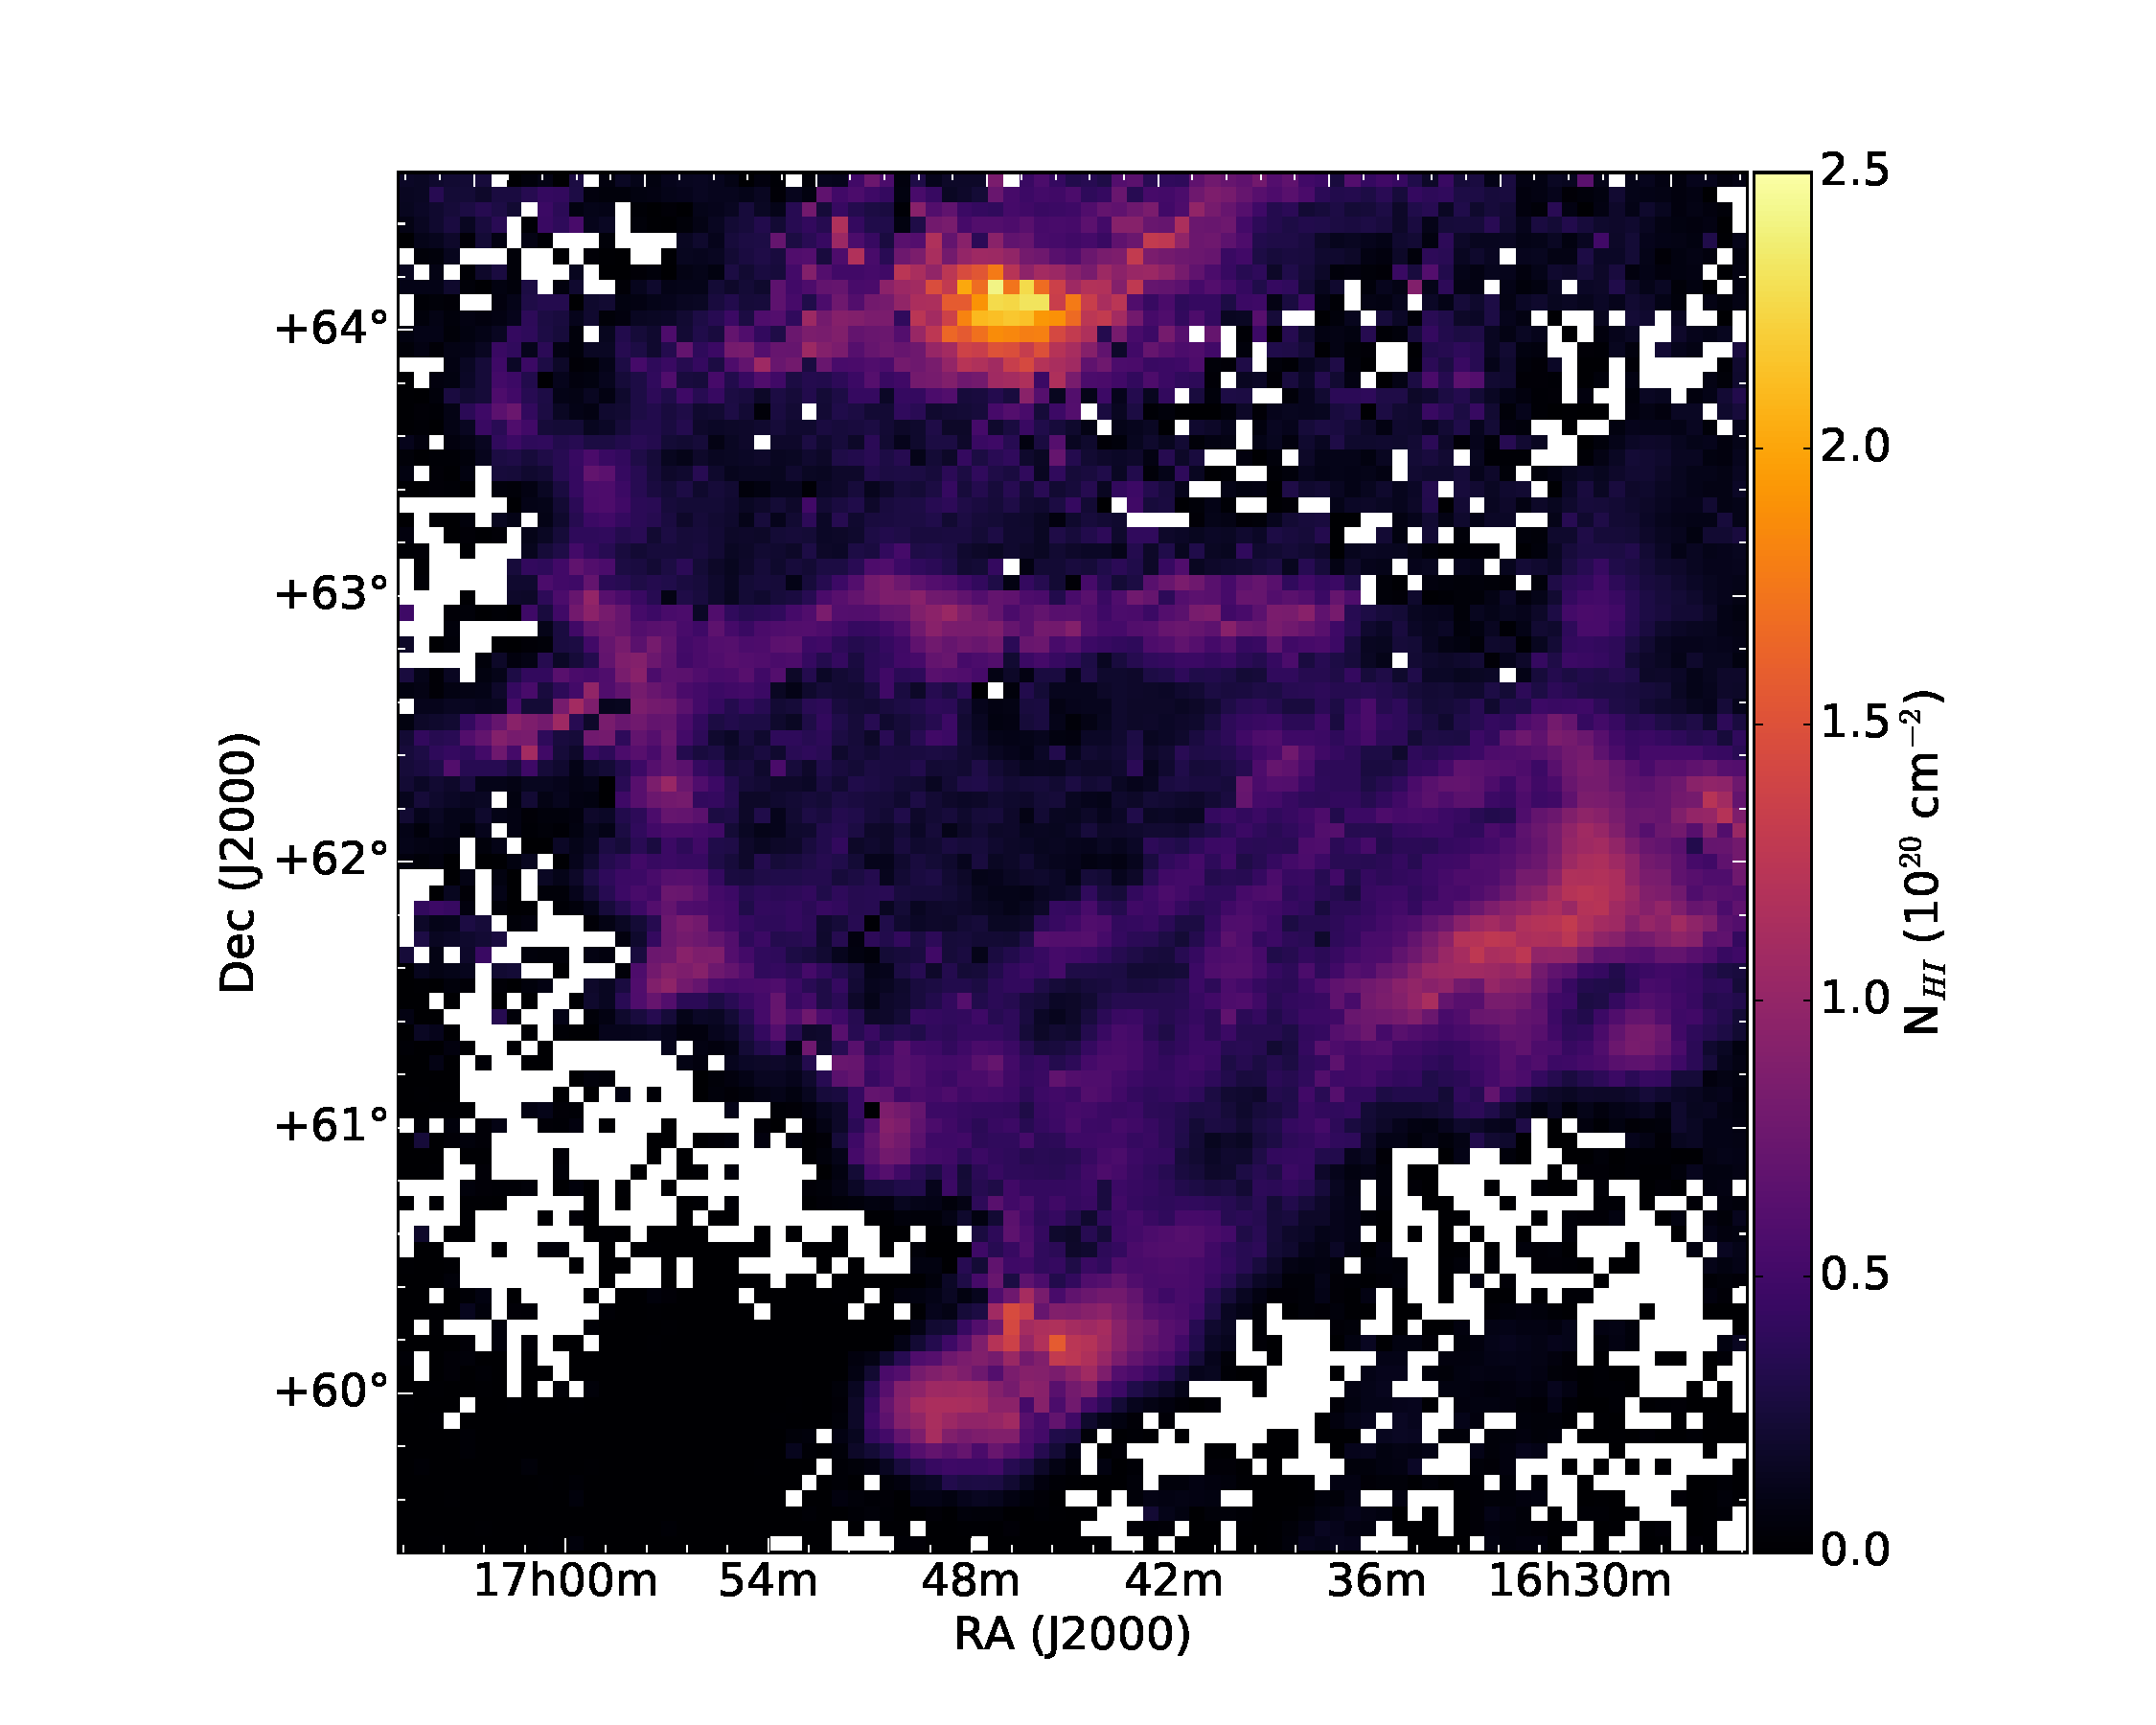
\includegraphics[page=1,height=7.5cm,trim=110 35 105 75,clip=true]{Figures/Phases_GHIGLS/GHIGLS_NHI.pdf}
   \hspace{5mm}
   \includegraphics[page=4,height=7.5cm,trim=110 35 105 75,clip=true]{Figures/Phases_GHIGLS/GHIGLS_NHI.pdf} \\
   \vspace{5mm}
   \includegraphics[page=2,height=7.5cm,trim=110 35 105 75,clip=true]{Figures/Phases_GHIGLS/GHIGLS_NHI.pdf}
   \hspace{5mm}
   \includegraphics[page=5,height=7.5cm,trim=110 35 105 75,clip=true]{Figures/Phases_GHIGLS/GHIGLS_NHI.pdf} \\
   \vspace{5mm}
   \includegraphics[page=3,height=7.5cm,trim=110 35 105 75,clip=true]{Figures/Phases_GHIGLS/GHIGLS_NHI.pdf}
   \hspace{5mm}
   \includegraphics[page=6,height=7.5cm,trim=110 35 105 75,clip=true]{Figures/Phases_GHIGLS/GHIGLS_NHI.pdf}
   \caption{\label{Phases_GHIGLS} Column density maps of the cold (\emph{left}) and warm (\emph{right}) phases of H\rmnum{1}. We separated the velocity components (from top to bottom: LVC+IVC, LVC, IVC).}
 \end{figure*}

%% \begin{figure*}[h]
   \centering
   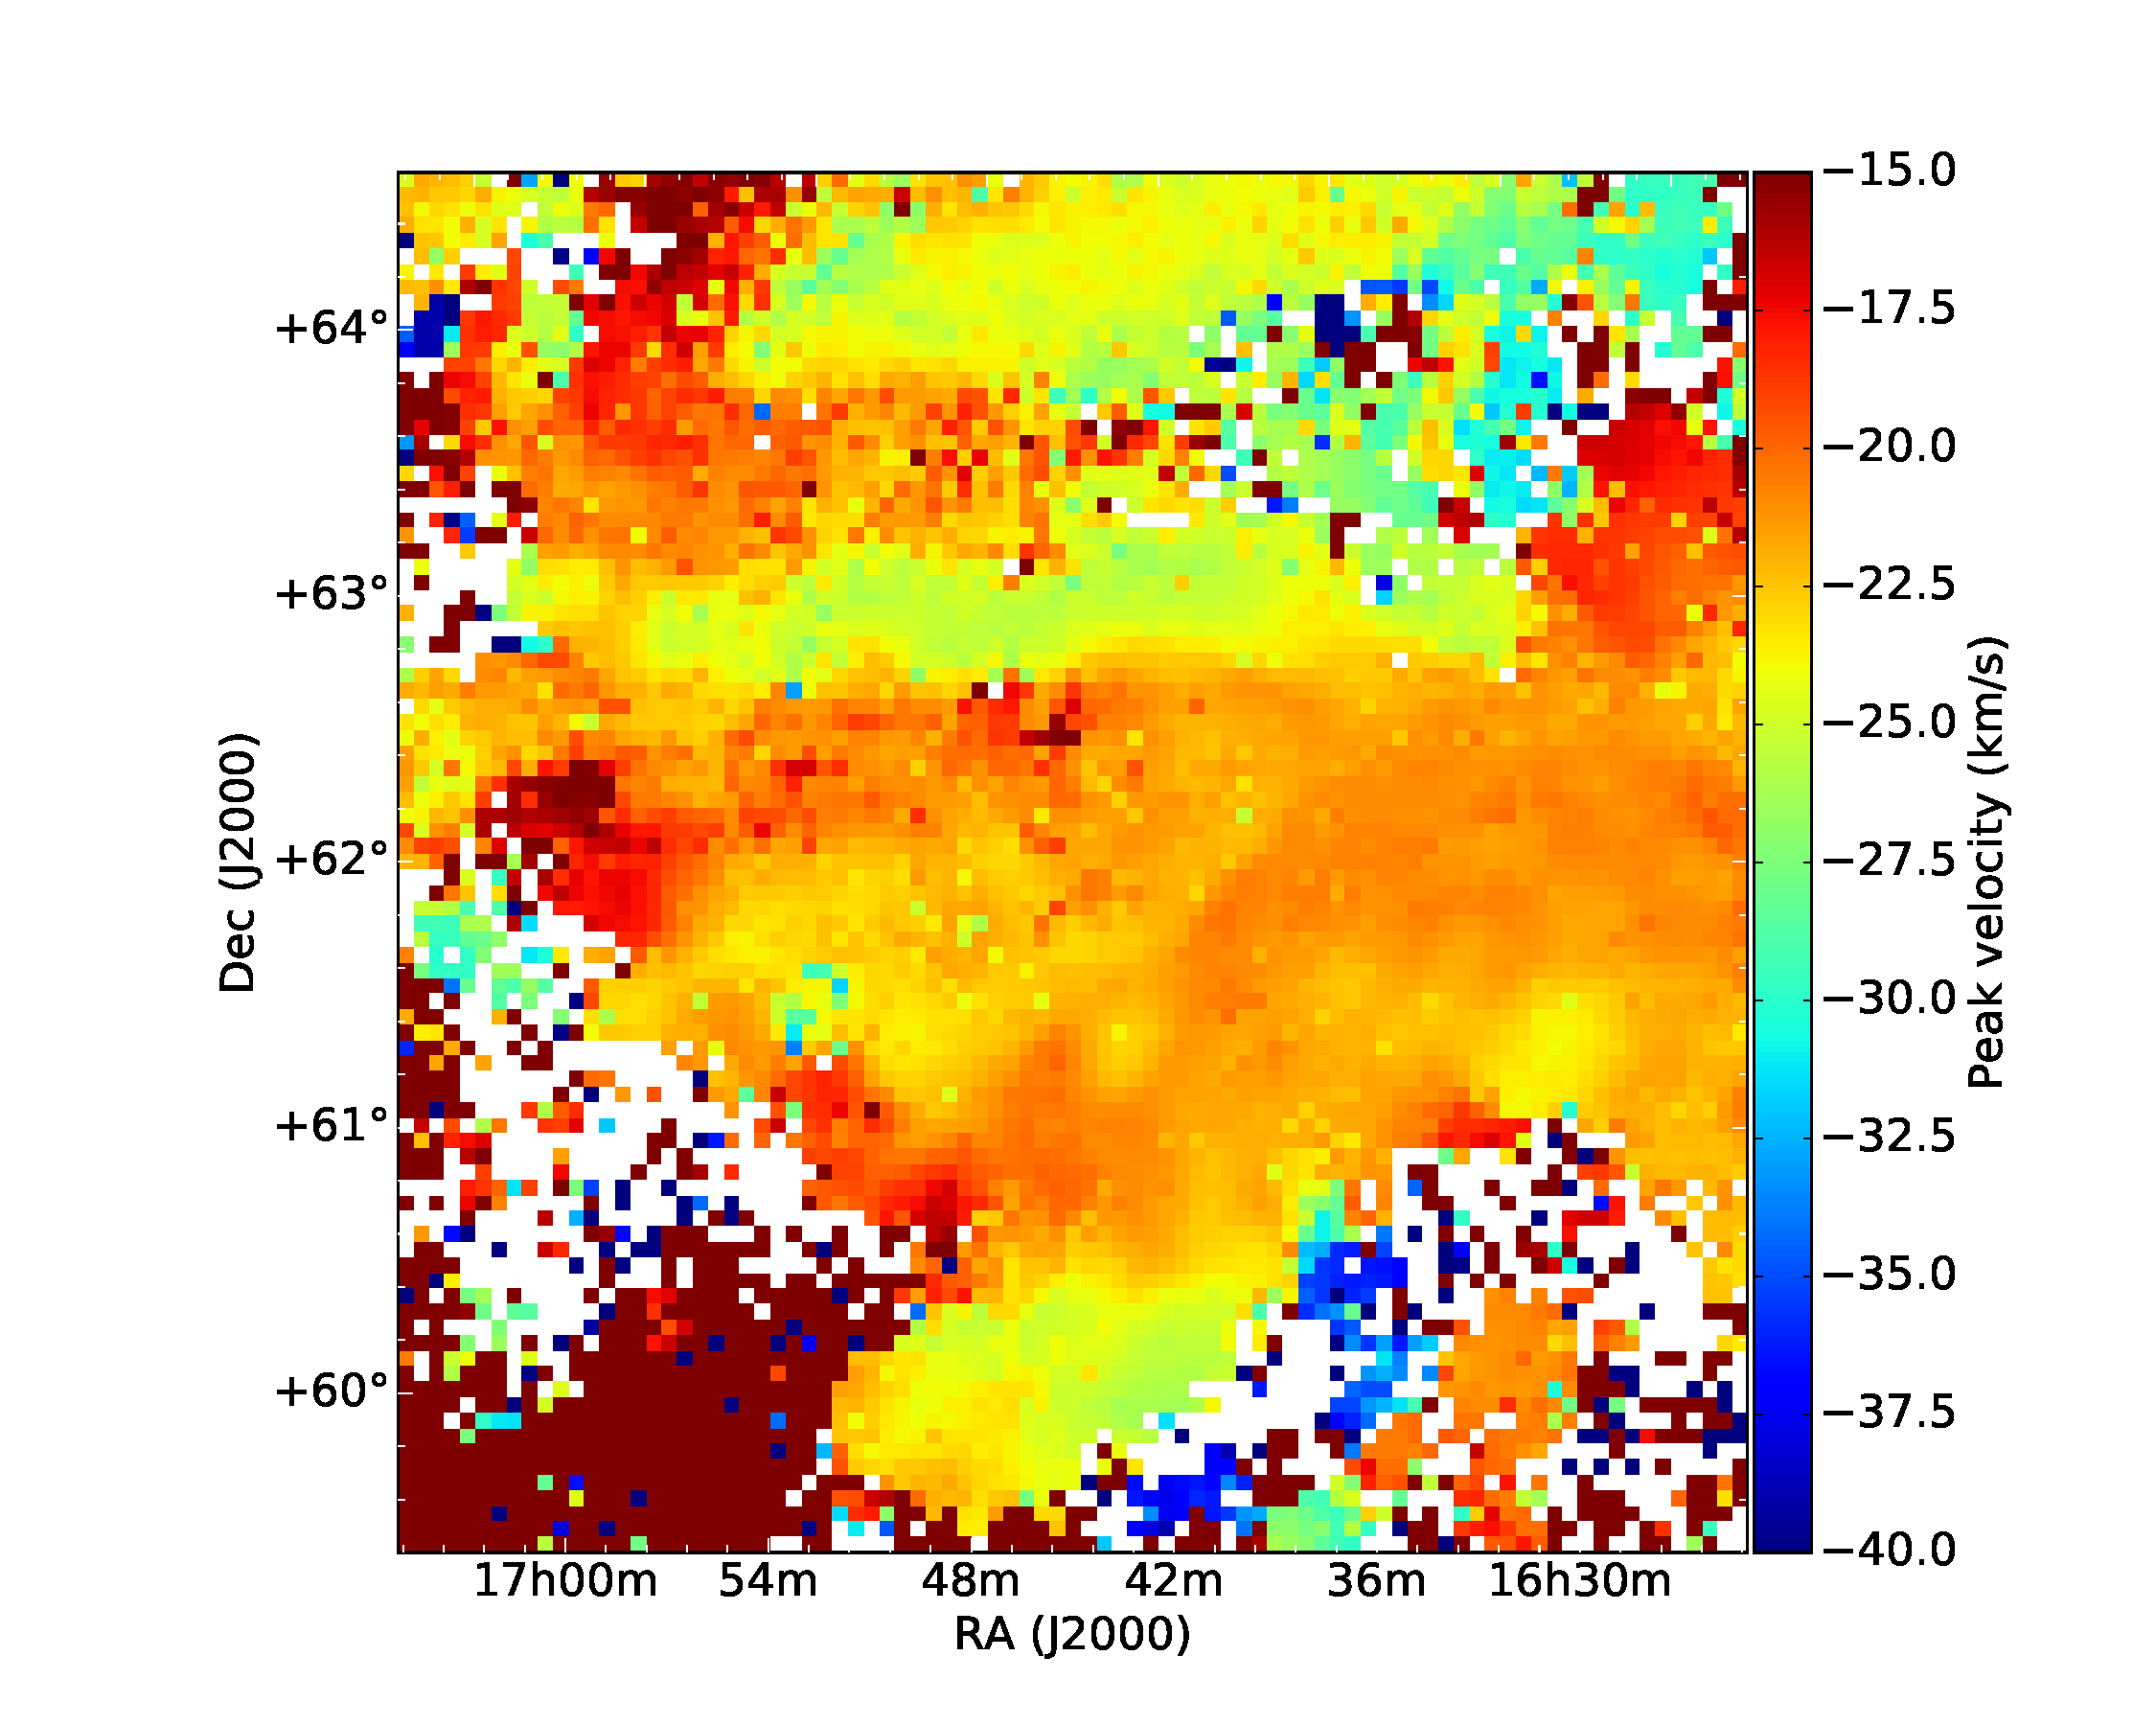
\includegraphics[page=1,height=7.5cm,trim=110 35 105 75,clip=true]{Figures/Phases_GHIGLS/GHIGLS_velo.pdf}
   \hspace{5mm}
   \includegraphics[page=4,height=7.5cm,trim=110 35 105 75,clip=true]{Figures/Phases_GHIGLS/GHIGLS_velo.pdf} \\
   \vspace{5mm}
   \includegraphics[page=2,height=7.5cm,trim=110 35 105 75,clip=true]{Figures/Phases_GHIGLS/GHIGLS_velo.pdf}
   \hspace{5mm}
   \includegraphics[page=5,height=7.5cm,trim=110 35 105 75,clip=true]{Figures/Phases_GHIGLS/GHIGLS_velo.pdf} \\
   \vspace{5mm}
   \includegraphics[page=3,height=7.5cm,trim=110 35 105 75,clip=true]{Figures/Phases_GHIGLS/GHIGLS_velo.pdf}
   \hspace{5mm}
   \includegraphics[page=6,height=7.5cm,trim=110 35 105 75,clip=true]{Figures/Phases_GHIGLS/GHIGLS_velo.pdf}
   \caption{Maps of the central velocity of the cold (\emph{left}) and warm (\emph{right}) phases of H\rmnum{1}. We separated the velocity components (from top to bottom: LVC+IVC, LVC, IVC).}
 \end{figure*}

%% \begin{figure*}[h]
   \centering
   \includegraphics[page=1,height=7.5cm,trim=110 35 105 75,clip=true]{Figures/Phases_GHIGLS/GHIGLS_disp.pdf}
   \hspace{5mm}
   \includegraphics[page=4,height=7.5cm,trim=110 35 105 75,clip=true]{Figures/Phases_GHIGLS/GHIGLS_disp.pdf} \\
   \vspace{5mm}
   \includegraphics[page=2,height=7.5cm,trim=110 35 105 75,clip=true]{Figures/Phases_GHIGLS/GHIGLS_disp.pdf}
   \hspace{5mm}
   \includegraphics[page=5,height=7.5cm,trim=110 35 105 75,clip=true]{Figures/Phases_GHIGLS/GHIGLS_disp.pdf} \\
   \vspace{5mm}
   \includegraphics[page=3,height=7.5cm,trim=110 35 105 75,clip=true]{Figures/Phases_GHIGLS/GHIGLS_disp.pdf}
   \hspace{5mm}
   \includegraphics[page=6,height=7.5cm,trim=110 35 105 75,clip=true]{Figures/Phases_GHIGLS/GHIGLS_disp.pdf}
   \caption{Maps of velocity dispersion of the cold (\emph{left}) and warm (\emph{right}) phases of H\rmnum{1}. We separated the velocity components (from top to bottom: LVC+IVC, LVC, IVC).}
 \end{figure*}

%% \begin{figure*}[h]
   \centering
   \includegraphics[page=1,height=7.5cm,trim=110 35 105 75,clip=true]{Figures/Phases_DHIGLS/DHIGLS_NHI.pdf}
   \hspace{5mm}
   \includegraphics[page=4,height=7.5cm,trim=110 35 105 75,clip=true]{Figures/Phases_DHIGLS/DHIGLS_NHI.pdf} \\
   \vspace{5mm}
   \includegraphics[page=2,height=7.5cm,trim=110 35 105 75,clip=true]{Figures/Phases_DHIGLS/DHIGLS_NHI.pdf}
   \hspace{5mm}
   \includegraphics[page=5,height=7.5cm,trim=110 35 105 75,clip=true]{Figures/Phases_DHIGLS/DHIGLS_NHI.pdf} \\
   \vspace{5mm}
   \includegraphics[page=3,height=7.5cm,trim=110 35 105 75,clip=true]{Figures/Phases_DHIGLS/DHIGLS_NHI.pdf}
   \hspace{5mm}
   \includegraphics[page=6,height=7.5cm,trim=110 35 105 75,clip=true]{Figures/Phases_DHIGLS/DHIGLS_NHI.pdf}
   \caption{\label{Phases_DHIGLS} Column density maps of the cold (\emph{left}) and warm (\emph{right}) phases of H\rmnum{1}. We separated the velocity components (from top to bottom: LVC+IVC, LVC, IVC).}
 \end{figure*}

%% \begin{figure*}[h]
   \centering
   \includegraphics[page=1,height=7.5cm,trim=110 35 105 75,clip=true]{Figures/Phases_DHIGLS/DHIGLS_velo.pdf}
   \hspace{5mm}
   \includegraphics[page=4,height=7.5cm,trim=110 35 105 75,clip=true]{Figures/Phases_DHIGLS/DHIGLS_velo.pdf} \\
   \vspace{5mm}
   \includegraphics[page=2,height=7.5cm,trim=110 35 105 75,clip=true]{Figures/Phases_DHIGLS/DHIGLS_velo.pdf}
   \hspace{5mm}
   \includegraphics[page=5,height=7.5cm,trim=110 35 105 75,clip=true]{Figures/Phases_DHIGLS/DHIGLS_velo.pdf} \\
   \vspace{5mm}
   \includegraphics[page=3,height=7.5cm,trim=110 35 105 75,clip=true]{Figures/Phases_DHIGLS/DHIGLS_velo.pdf}
   \hspace{5mm}
   \includegraphics[page=6,height=7.5cm,trim=110 35 105 75,clip=true]{Figures/Phases_DHIGLS/DHIGLS_velo.pdf}
   \caption{Maps of the central velocity of the cold (\emph{left}) and warm (\emph{right}) phases of H\rmnum{1}. We separated the velocity components (from top to bottom: LVC+IVC, LVC, IVC).}
 \end{figure*}

%% \begin{figure*}[h]
   \centering
   \includegraphics[page=1,height=7.5cm,trim=110 35 105 75,clip=true]{Figures/Phases_DHIGLS/DHIGLS_disp.pdf}
   \hspace{5mm}
   \includegraphics[page=4,height=7.5cm,trim=110 35 105 75,clip=true]{Figures/Phases_DHIGLS/DHIGLS_disp.pdf} \\
   \vspace{5mm}
   \includegraphics[page=2,height=7.5cm,trim=110 35 105 75,clip=true]{Figures/Phases_DHIGLS/DHIGLS_disp.pdf}
   \hspace{5mm}
   \includegraphics[page=5,height=7.5cm,trim=110 35 105 75,clip=true]{Figures/Phases_DHIGLS/DHIGLS_disp.pdf} \\
   \vspace{5mm}
   \includegraphics[page=3,height=7.5cm,trim=110 35 105 75,clip=true]{Figures/Phases_DHIGLS/DHIGLS_disp.pdf}
   \hspace{5mm}
   \includegraphics[page=6,height=7.5cm,trim=110 35 105 75,clip=true]{Figures/Phases_DHIGLS/DHIGLS_disp.pdf}
   \caption{Maps of velocity dispersion of the cold (\emph{left}) and warm (\emph{right}) phases of H\rmnum{1}. We separated the velocity components (from top to bottom: LVC+IVC, LVC, IVC).}
 \end{figure*}
\end{document}


